\subsection{Parameter scans on masses, couplings and mixing angles}

\paragraph{Logic of how we proceeded}

\begin{itemize}
\item Starting from benchmark 3 of \cite{Bauer:2017ota}
\item Mapping the kinematics and sensitivity of the model by scanning some of the
various parameters
\item Checking whether other existing models can be rescaled
\end{itemize}

\subsubsection{Results of studies}

Each of the signatures should have the following plots in the planes
of the final recommendation: 
\begin{itemize} 
\item efficiency at parton level with simplified, published cuts
\item total and fiducial cross-section at parton level 
\item 2 - 3 kinematic plots of what has been scanned that are most representative for the analysis (here the analysers decide, then we harmonize at the end)
\end{itemize} 

Signatures:

\begin{itemize}

\item{Mono-Z (lep/had)}

\item{MonoH$\rightarrow$bb}

\item{Monojet}

\item{ttbar+MET}, with specific discussion about rescaling

\item{other signatures who have not yet presented at public meetings, in ATLAS and CMS}

\end{itemize}

\subsubsection{Studies of the $\monohbb$ signature}
\subparagraph{Sensitivity estimate}

\begin{figure}[tbp]
\centering
\begin{subfigure}{0.48\textwidth}
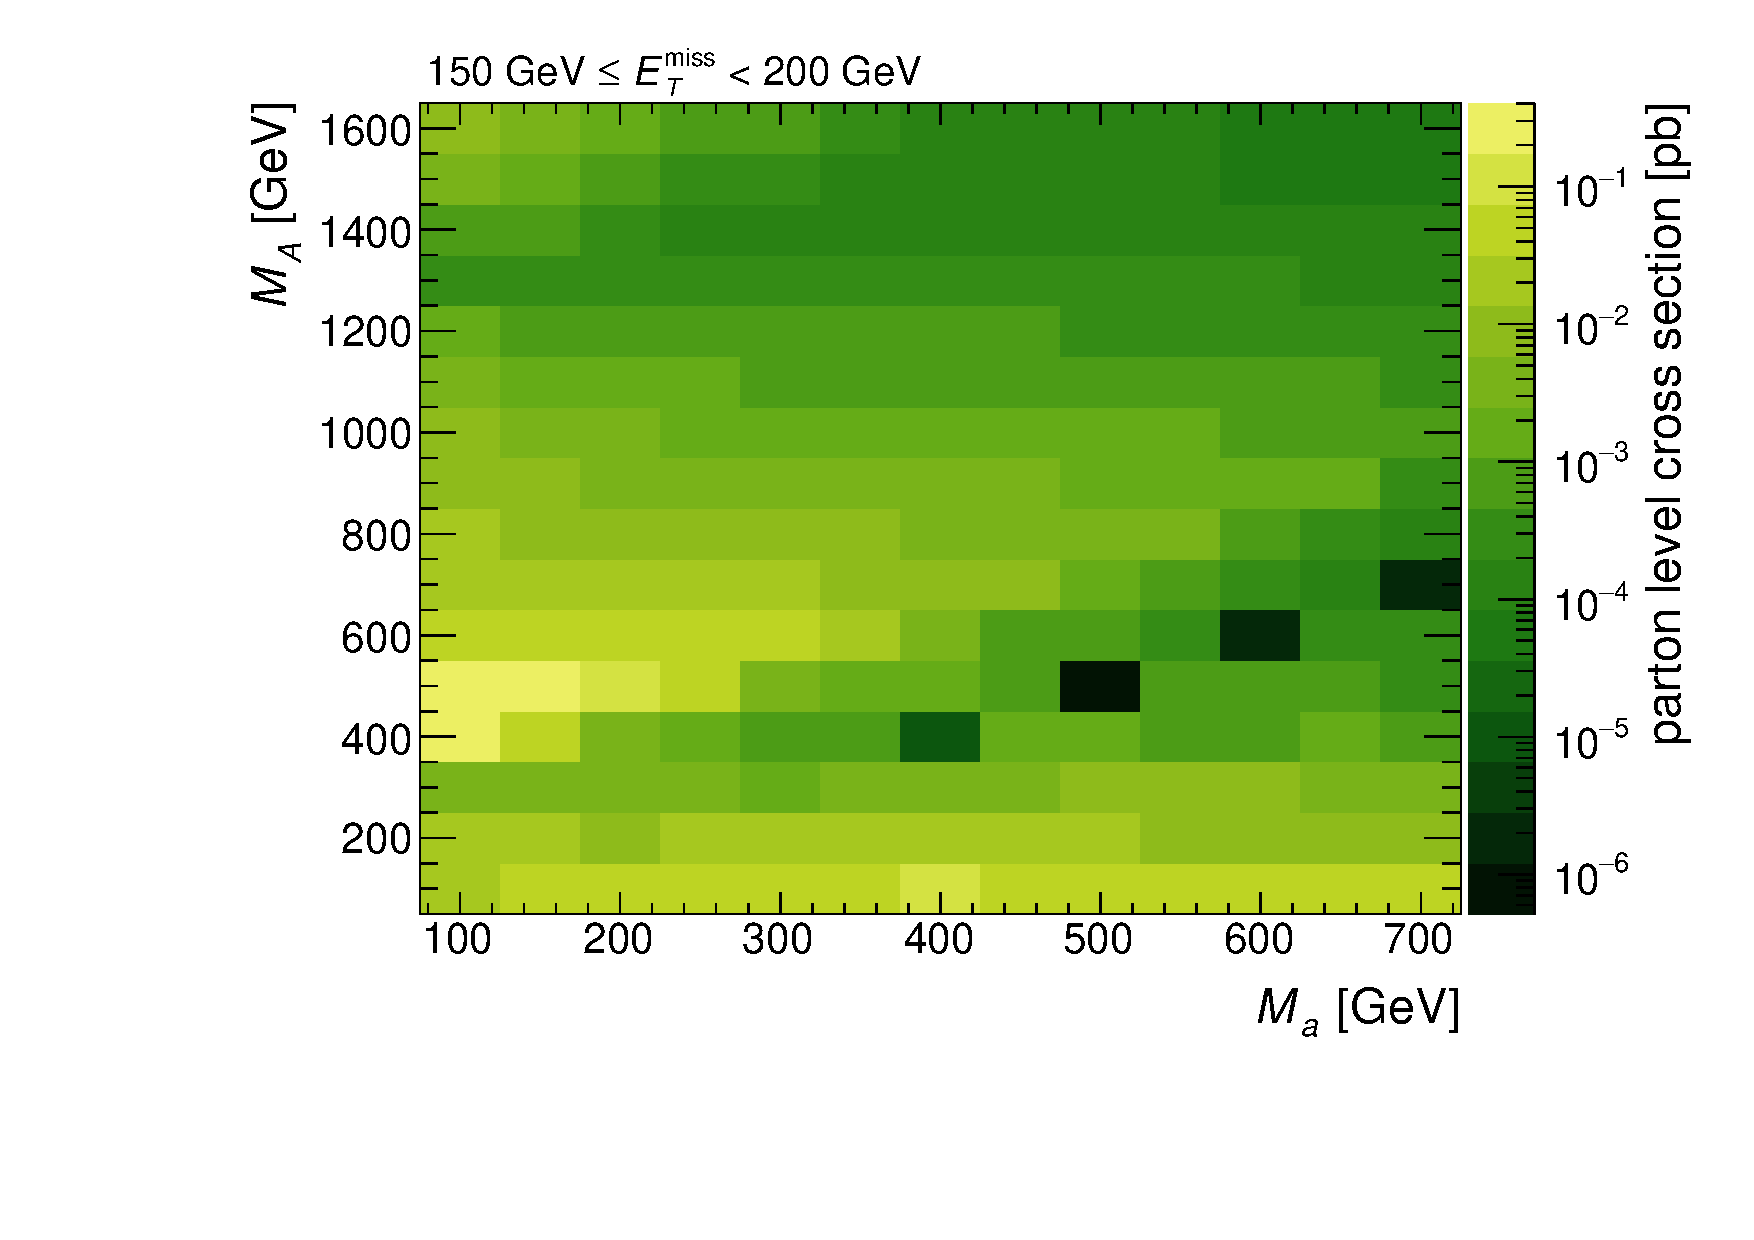
\includegraphics[width = \textwidth]{texinputs/04_grid/figures/monoHbb_parton_level_cross_section_bin_1_ma_vs_mA_lin.pdf}
\end{subfigure}
~
\begin{subfigure}{0.48\textwidth}
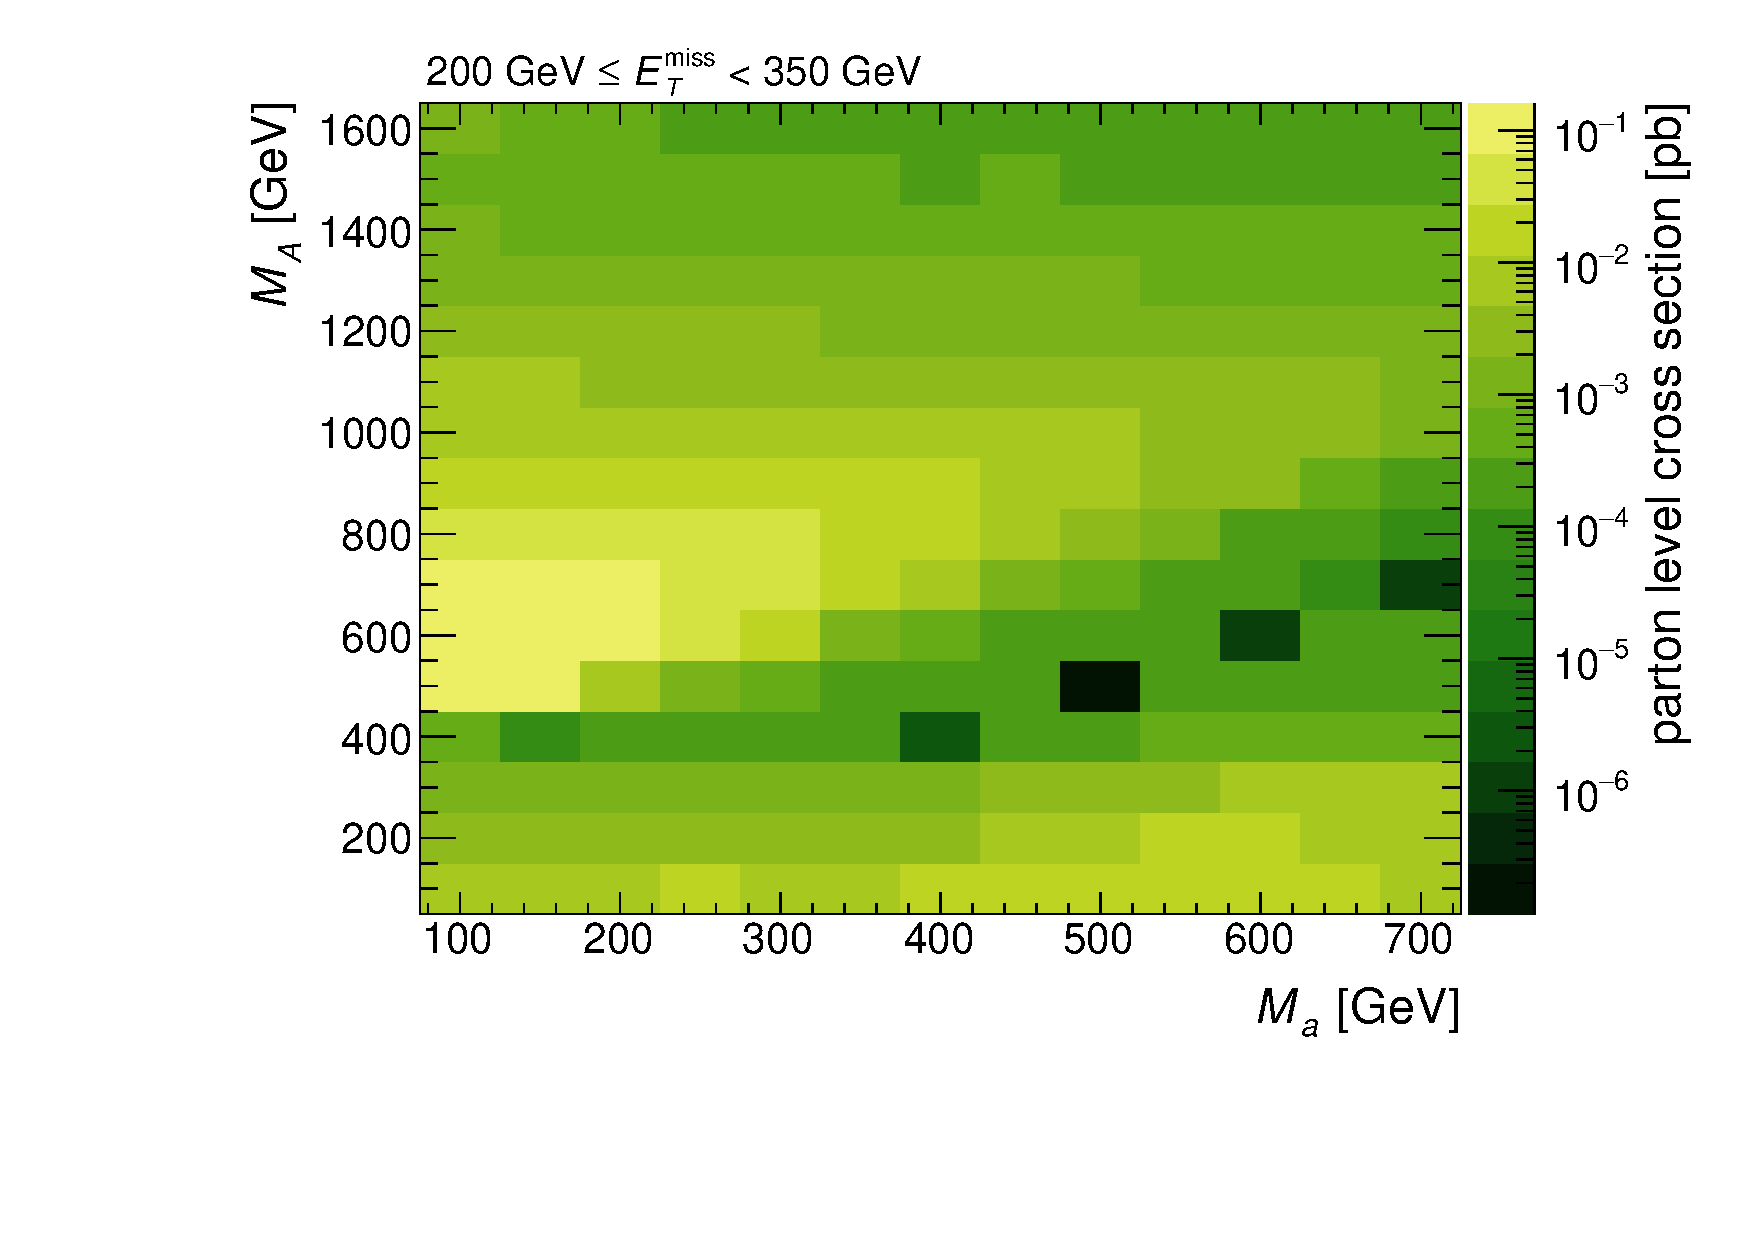
\includegraphics[width = \textwidth]{texinputs/04_grid/figures/monoHbb_parton_level_cross_section_bin_2_ma_vs_mA_lin.pdf}
\end{subfigure}
\\
\centering
\begin{subfigure}{0.48\textwidth}
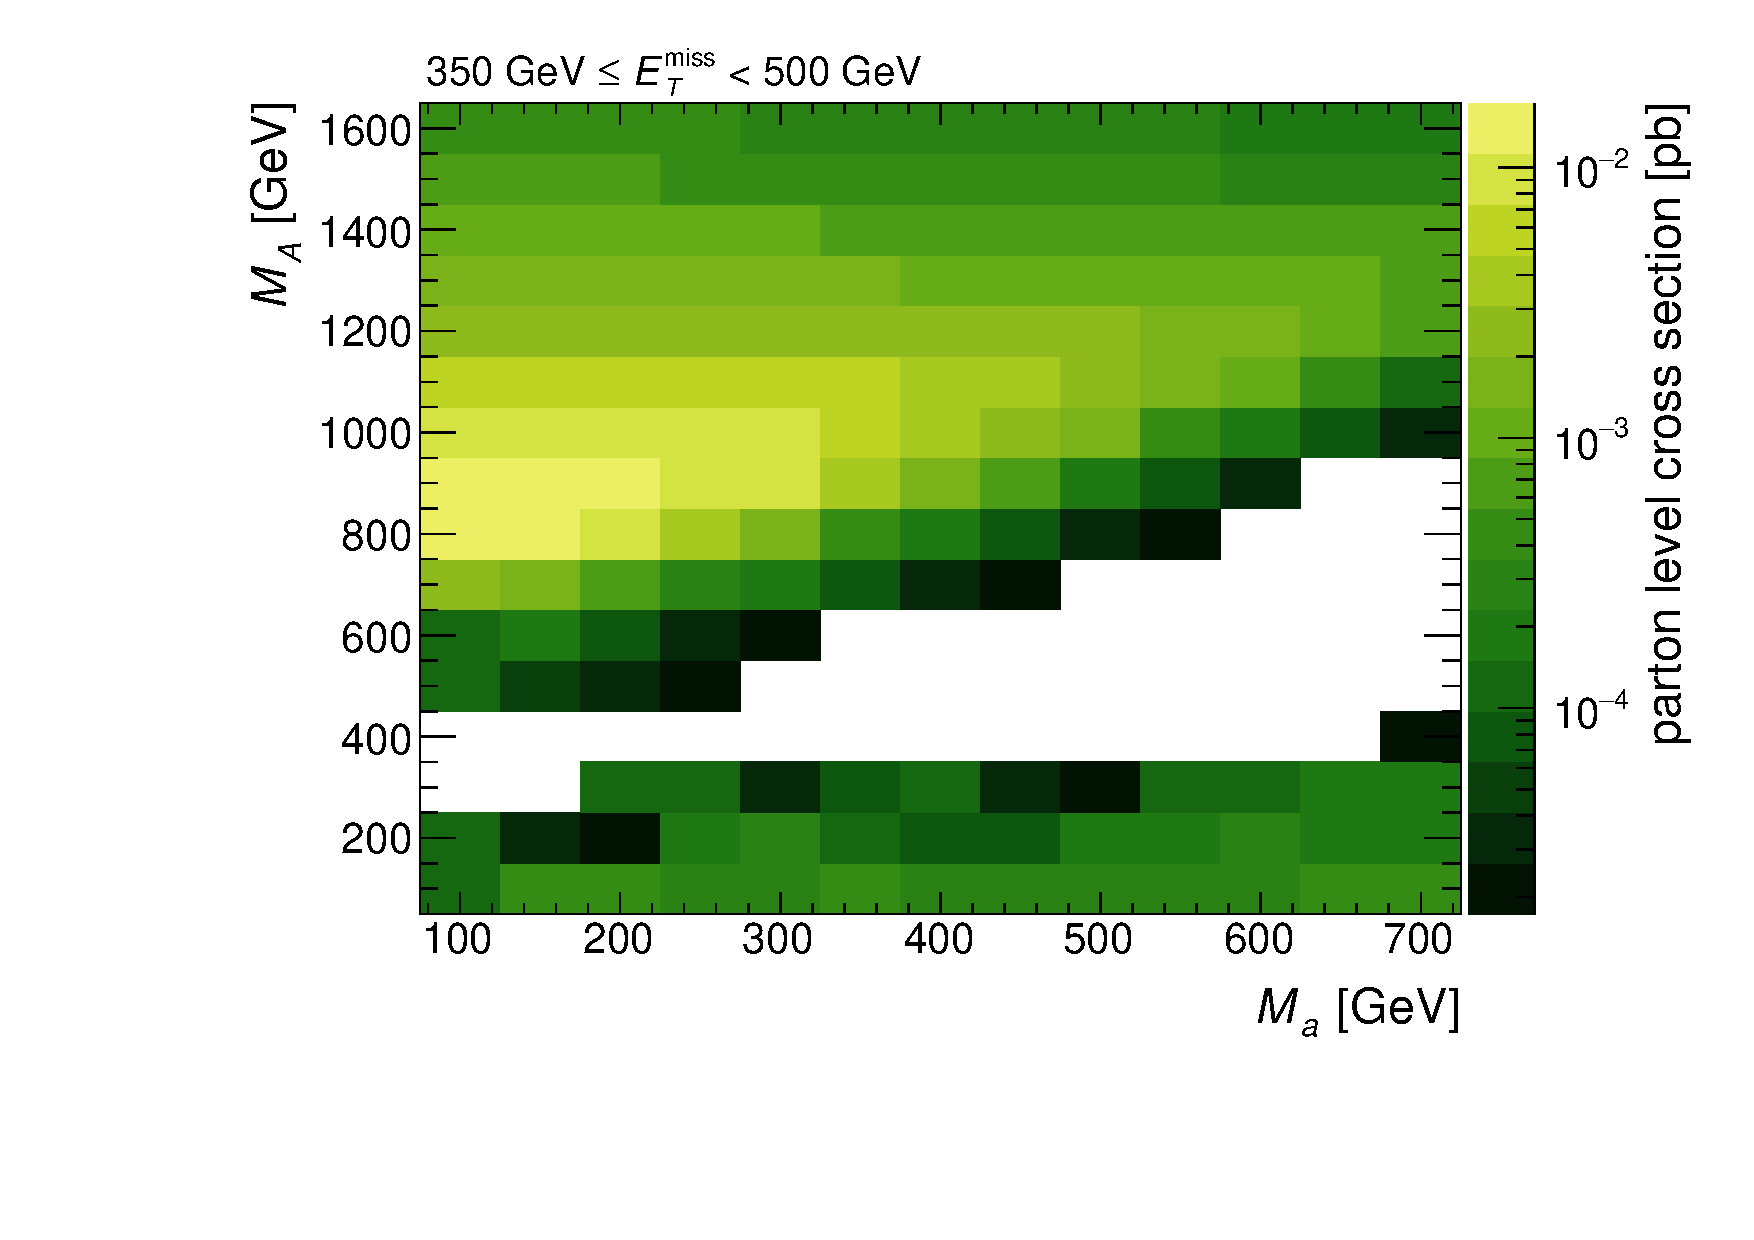
\includegraphics[width = \textwidth]{texinputs/04_grid/figures/monoHbb_parton_level_cross_section_bin_3_ma_vs_mA_lin.pdf}
\end{subfigure}
~
\begin{subfigure}{0.48\textwidth}
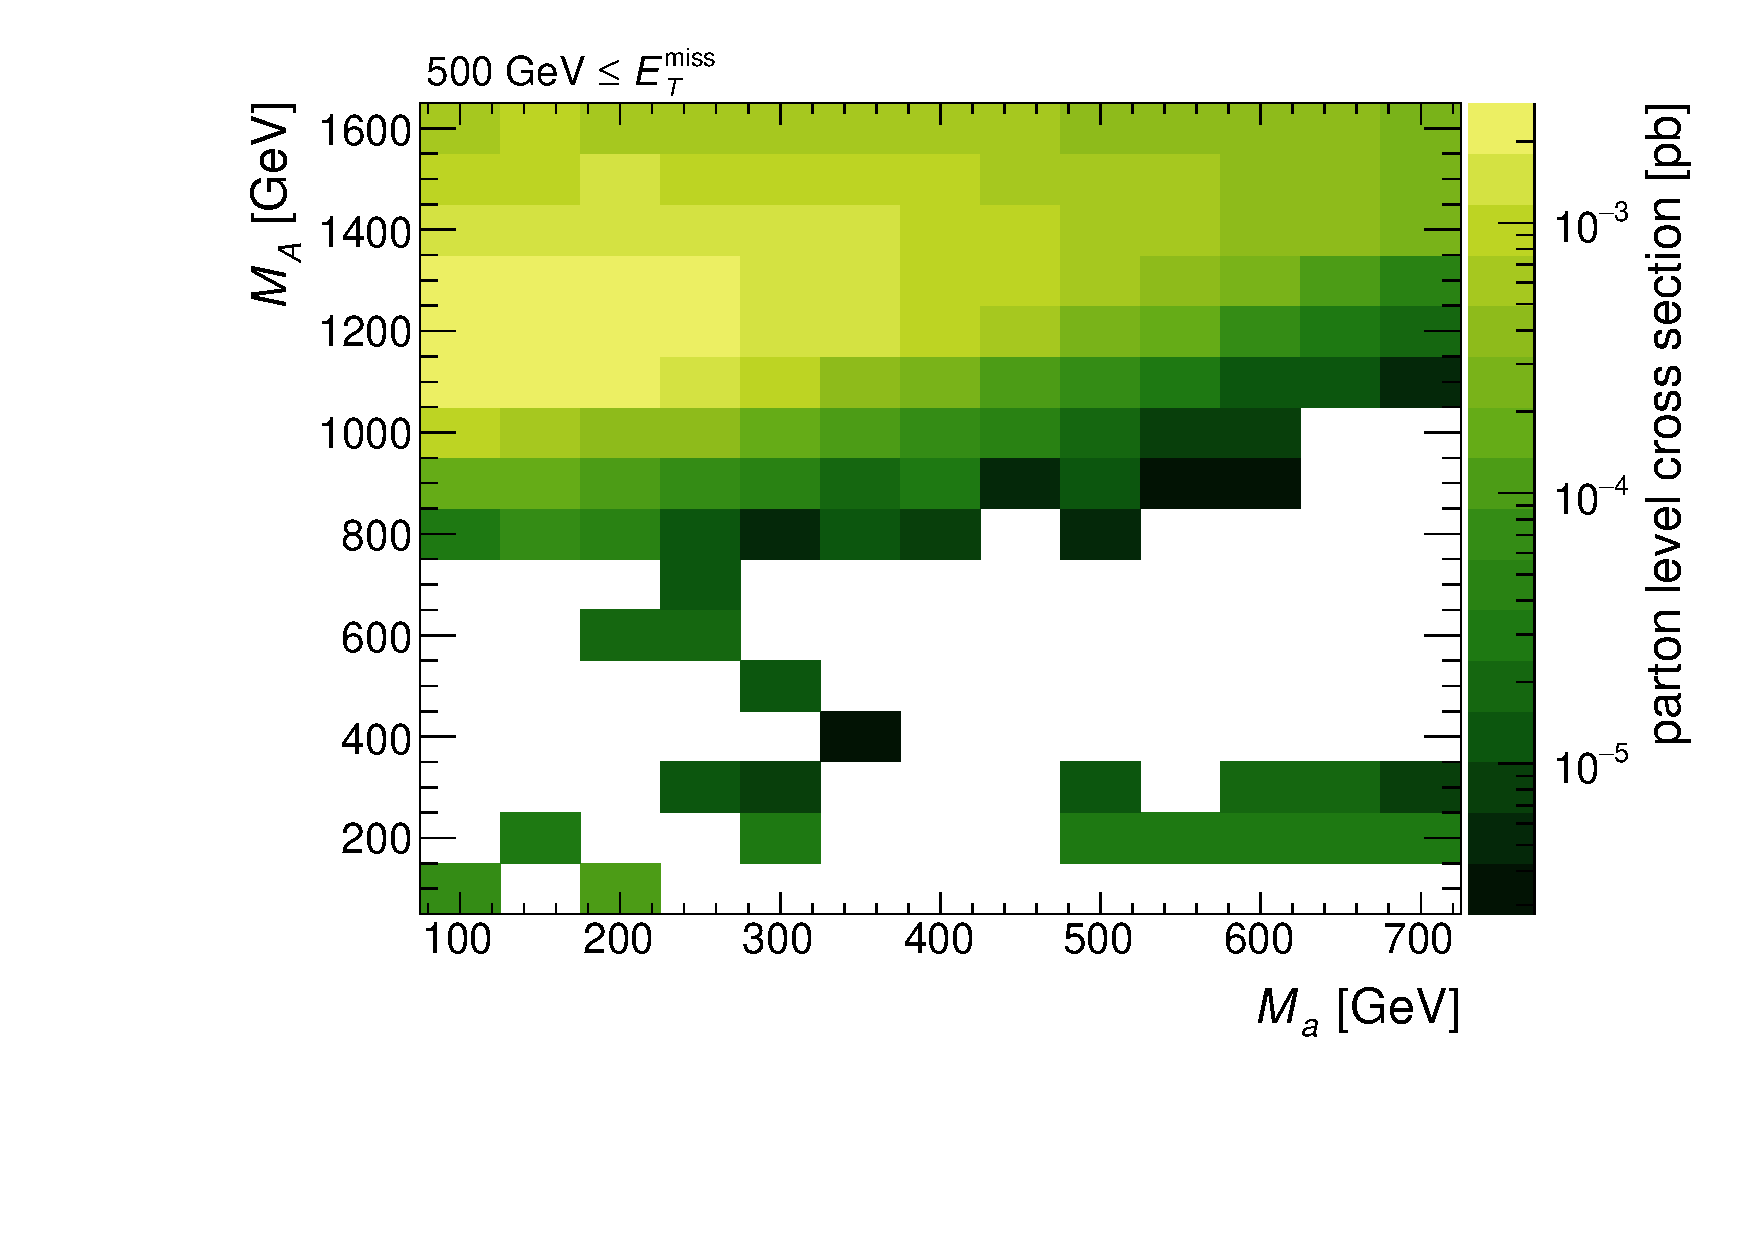
\includegraphics[width = \textwidth]{texinputs/04_grid/figures/monoHbb_parton_level_cross_section_bin_4_ma_vs_mA_lin.pdf}
\end{subfigure}
\caption[$h\to bb + \MET$ cross section binned in $\MET$, $\mA$ - $\ma$ plane ]
{
The production cross section of $h\to bb + \MET$ signal events at parton level as a function of $(\mA,\ma)$ in each of the four \met bins. 
The remaining parameters take the values
$ \mH=\mHc= \mA, \sinp = 0.35, \tanb = 1, \mDM = 10$ GeV and $ \lap1 = \lap2 = \lam3 = 3 $.
}
\label{fig:monoHbb_xsec_bins_mA_ma}
\end{figure}

\begin{figure}[tbp]
\centering
\begin{subfigure}{0.48\textwidth}
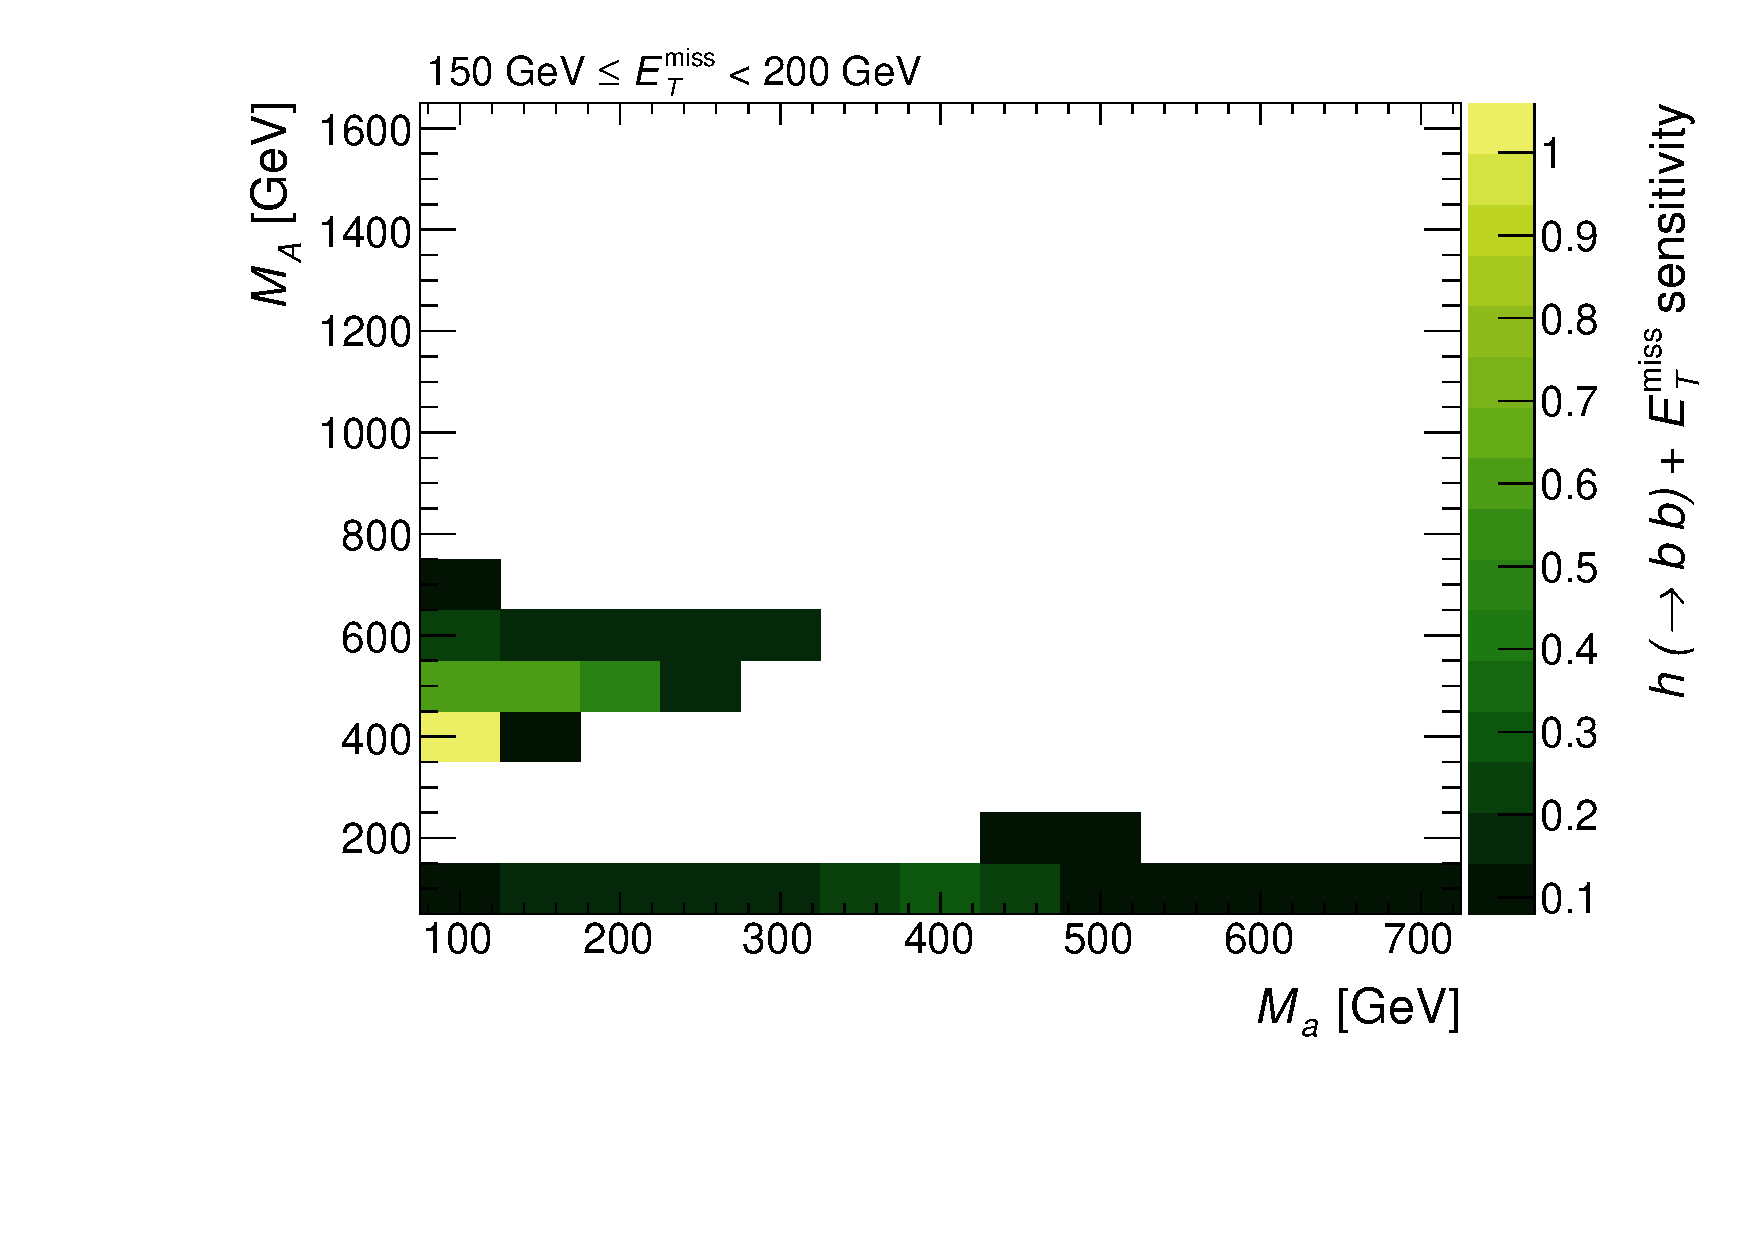
\includegraphics[width = \textwidth]{texinputs/04_grid/figures/monoHbb_sensi_bin_1_ma_vs_mA_lin.pdf}
\end{subfigure}
~
\begin{subfigure}{0.48\textwidth}
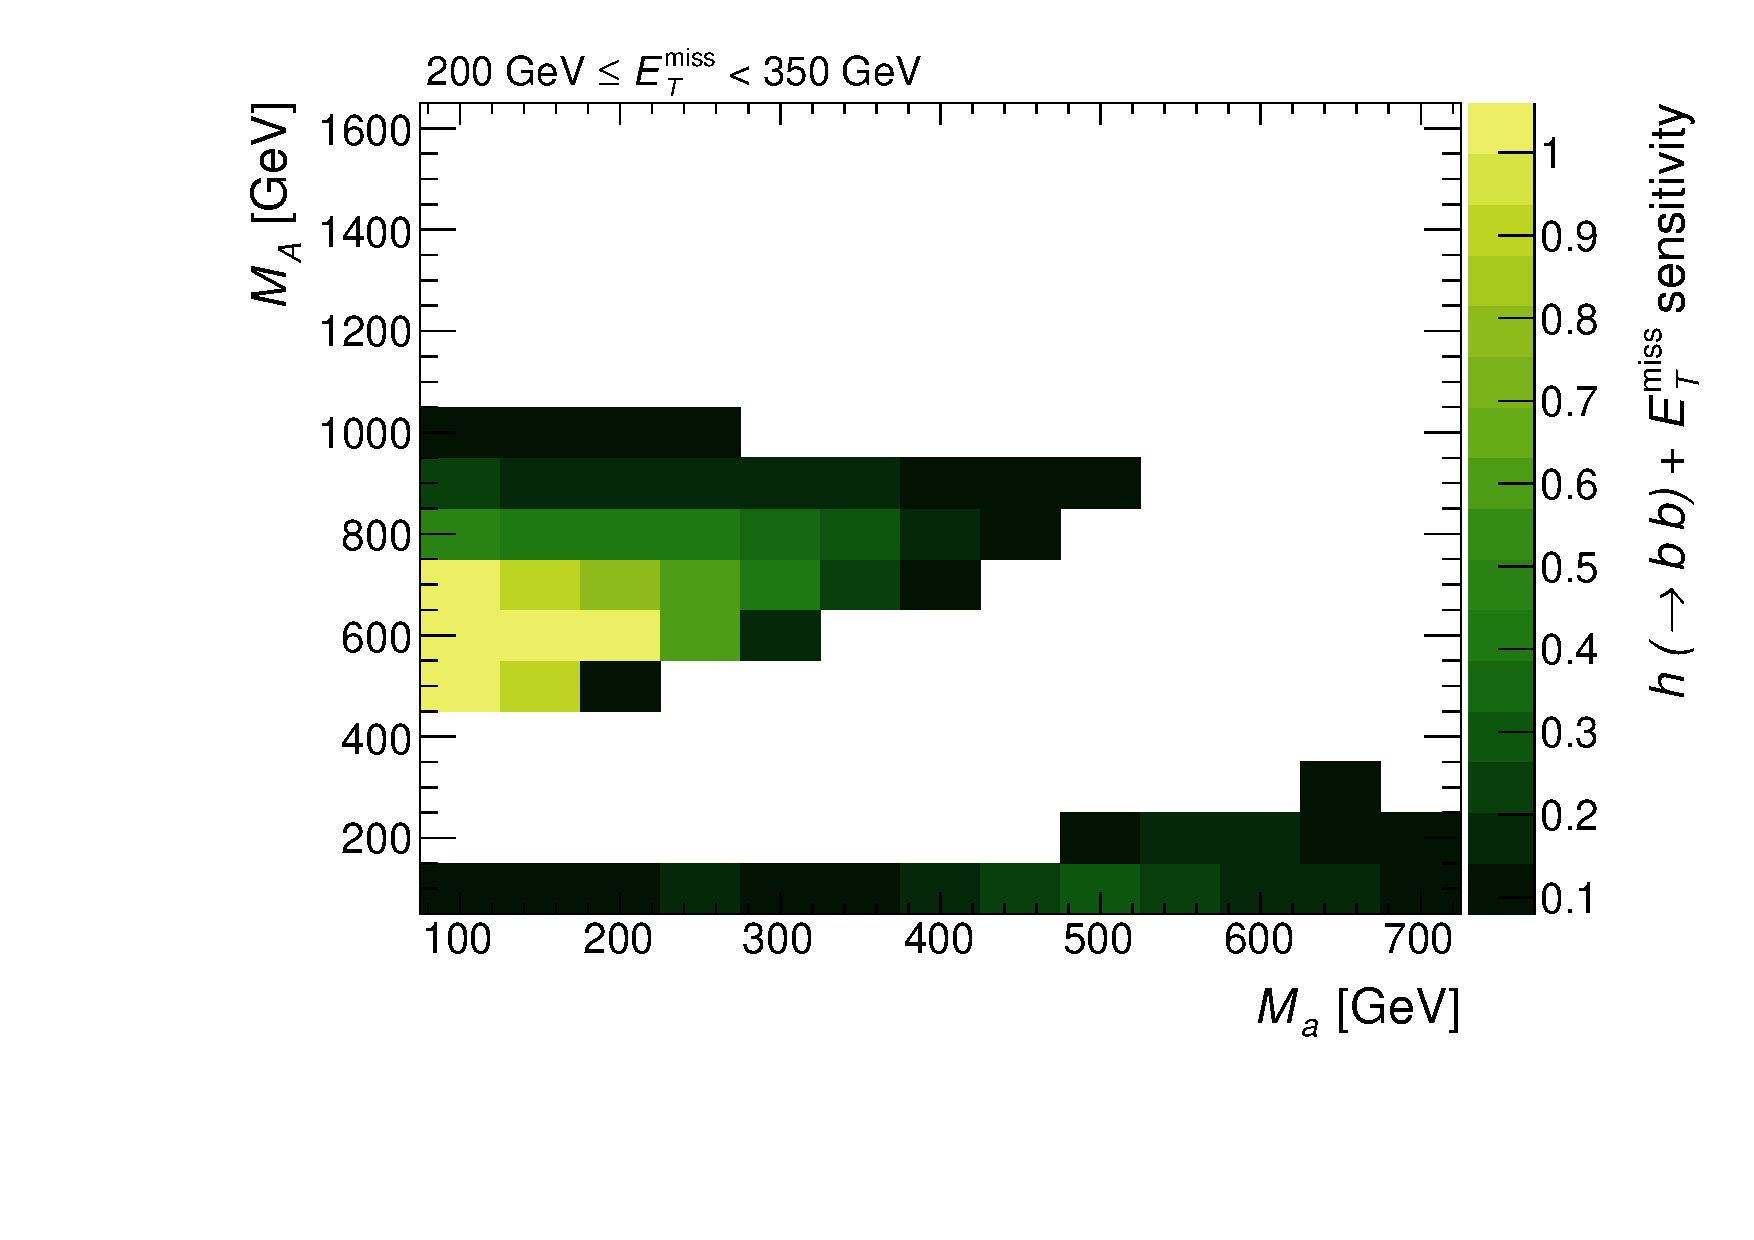
\includegraphics[width = \textwidth]{texinputs/04_grid/figures/monoHbb_sensi_bin_2_ma_vs_mA_lin.pdf}
\end{subfigure}
\\
\centering
\begin{subfigure}{0.48\textwidth}
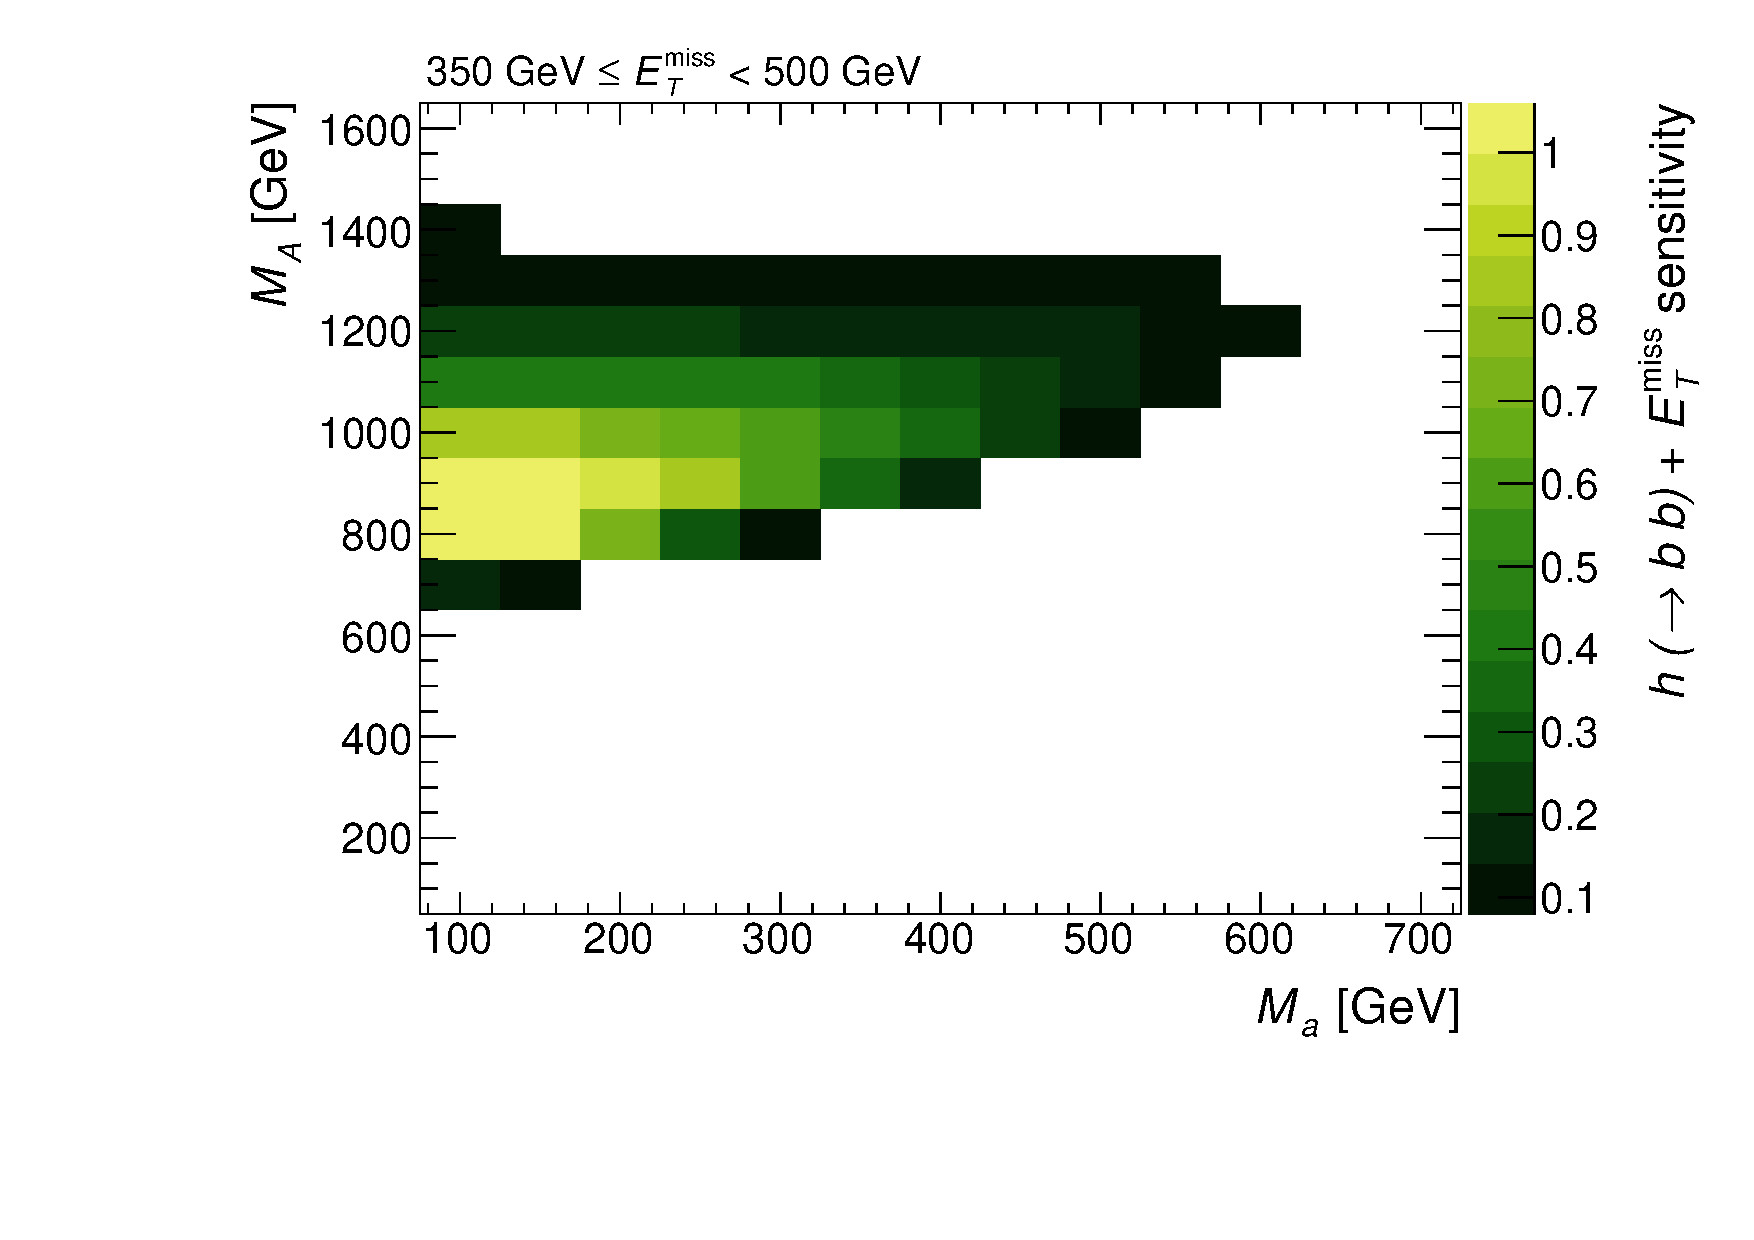
\includegraphics[width = \textwidth]{texinputs/04_grid/figures/monoHbb_sensi_bin_3_ma_vs_mA_lin.pdf}
\end{subfigure}
~
\begin{subfigure}{0.48\textwidth}
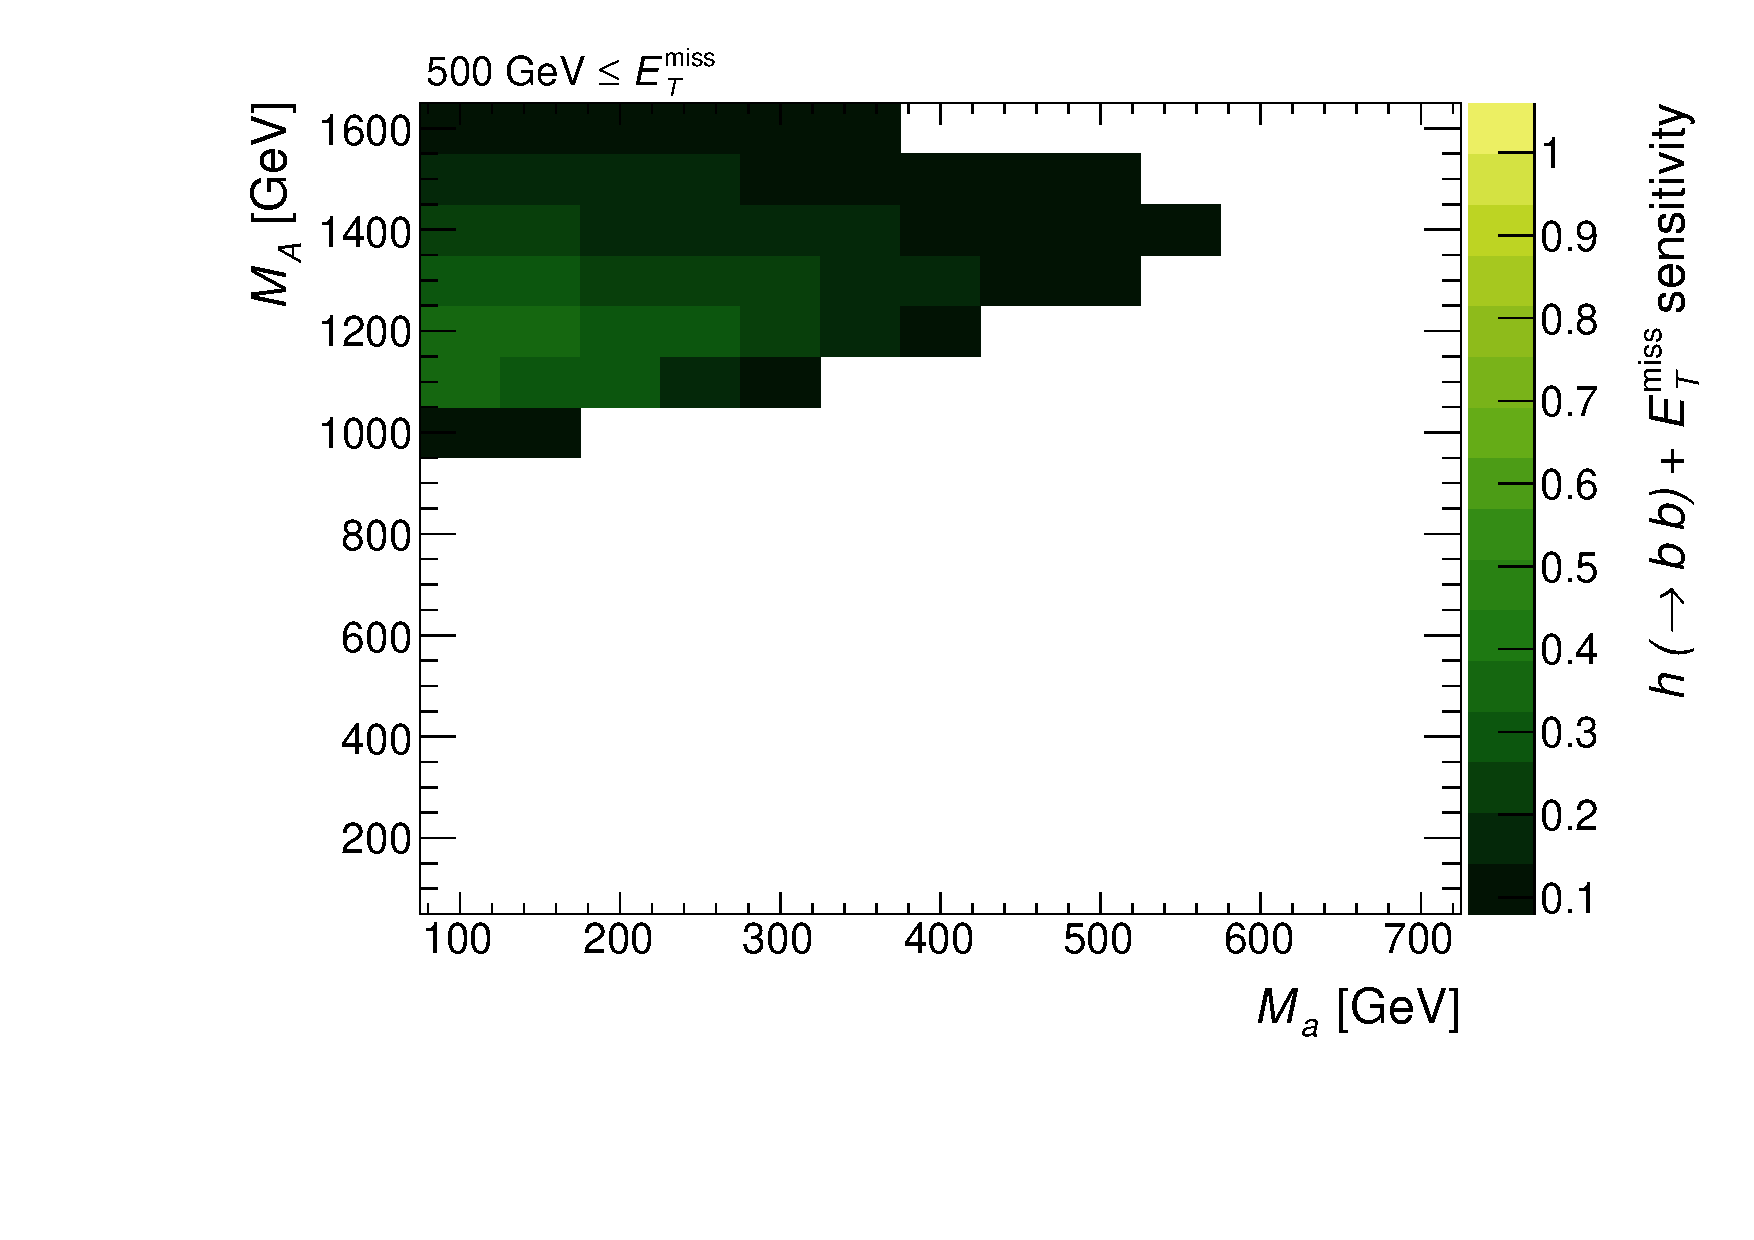
\includegraphics[width = \textwidth]{texinputs/04_grid/figures/monoHbb_sensi_bin_4_ma_vs_mA_lin.pdf}
\end{subfigure}
\caption[Sensitivity to the $h\to bb + \MET$ signal by $\MET$ bin, $\mA$ - $\ma$ plane]
{Estimated sensitivity to $h\to bb + \MET$ events as a function of $(\mA,\ma)$ in each of  the four \met bins. 
The sensitivity, defined in \autoref{eq:monoHbb_sensi}, is based on the limits with reduced model dependence from Ref.~\cite{Aaboud:2017yqz}. 
The remaining parameters take the values
$ \mH=\mHc= \mA, \sinp = 0.35, \tanb = 1, \mDM = 10$ GeV and $ \lap1 = \lap2 = \lam3 = 3 $.}
\label{fig:monoHbb_sensi_bins_mA_ma}
\end{figure}

%\begin{figure}[tbp]
%\centering
%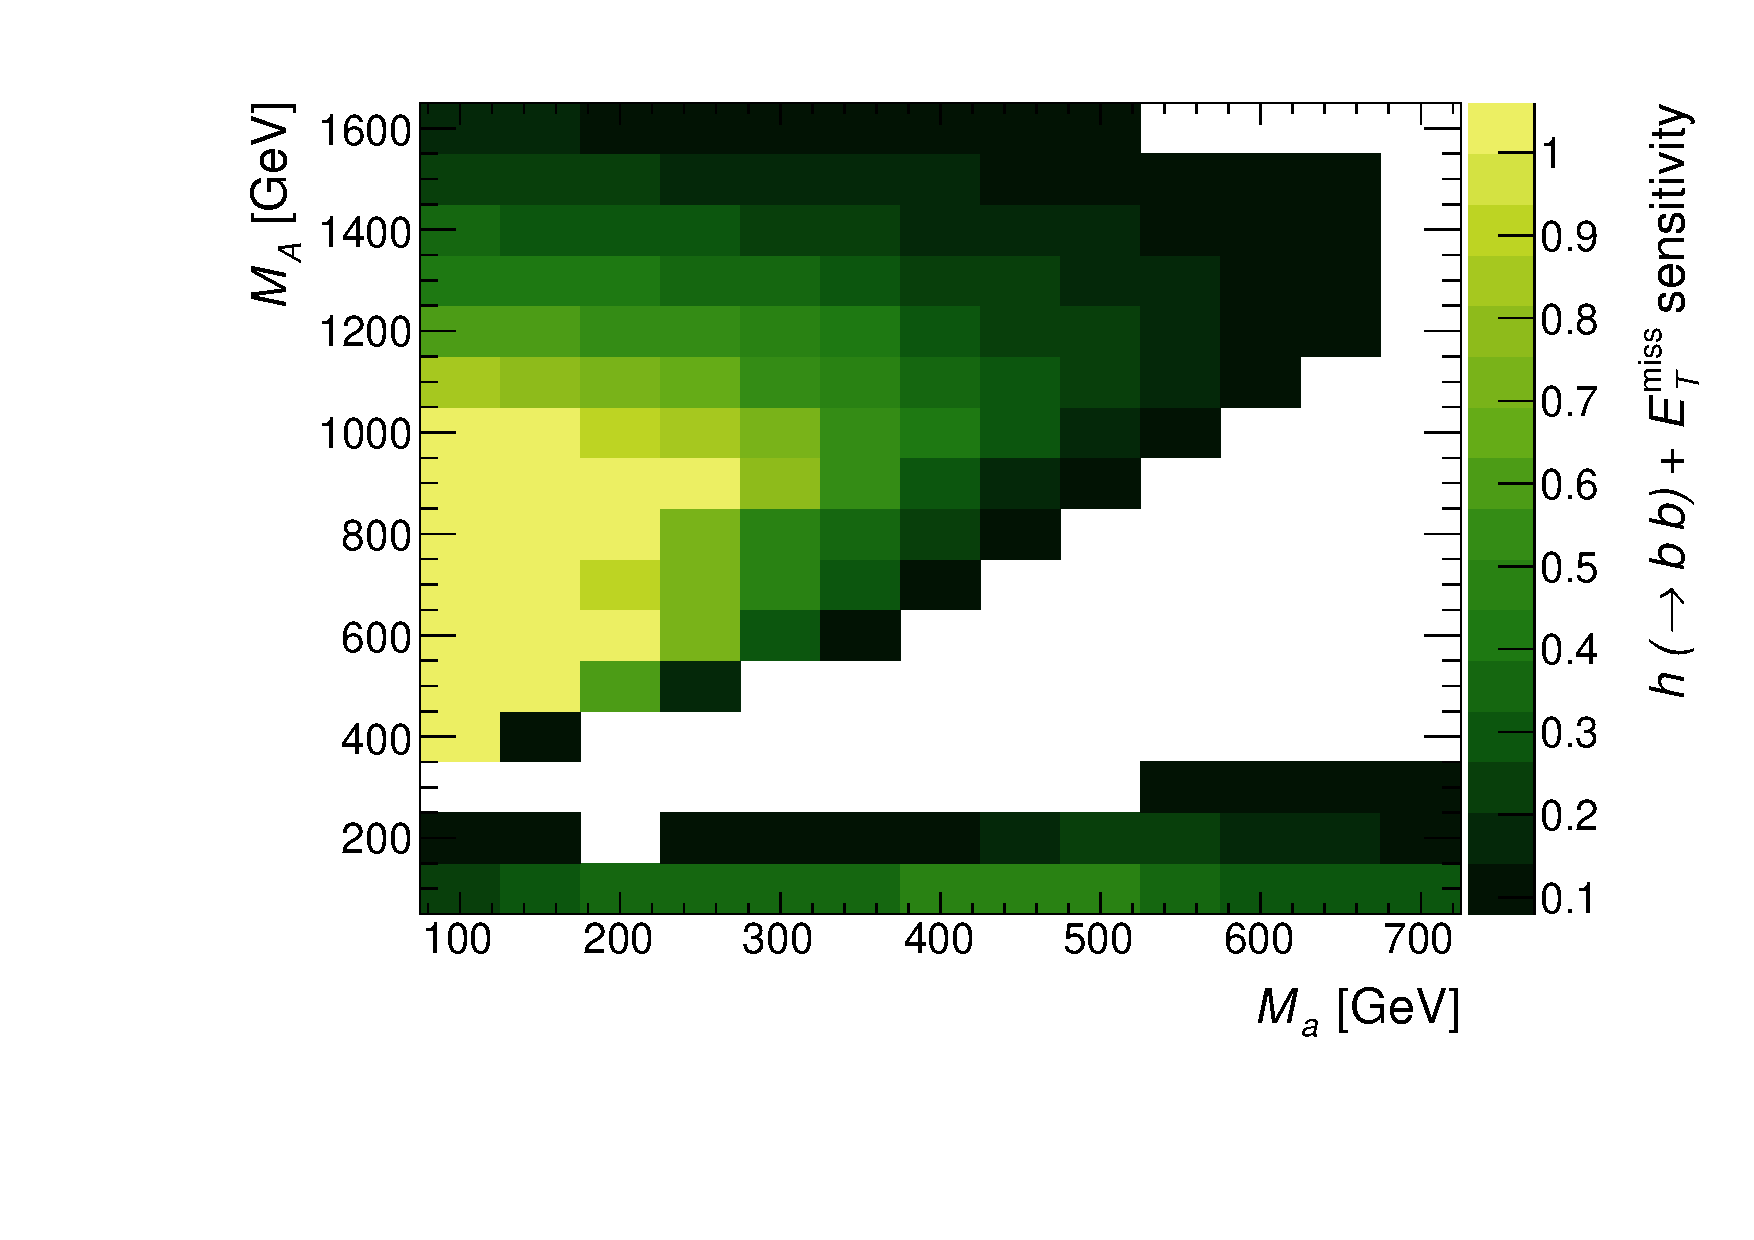
\includegraphics[width=0.7\textwidth]{texinputs/04_grid/figures/monoHbb_sensi_sum_bins_1_2_3_4_ma_vs_mA_lin.pdf}
%\caption[Sensitivity to $h\to bb + \MET$ signals in $\mA$ - $\ma$ plane, summed across $\MET$ bins]
%{
%Sum over all $\MET$-bins of the estimated sensitivity to $h\to bb + \MET$ events as a function of $(\mA,\ma)$. 
%The sensitivity, defined in \autoref{eq:monoHbb_sensi}, is based on the limits with reduced model dependence from Ref.~\cite{Aaboud:2017yqz}. 
%The remaining parameters take the values $ \mH=\mHc= \mA, \sinp = 0.35, \tanb = 1, \mDM = 10$ GeV and $ \lap1 = \lap2 = \lam3 = 3 $.}
%\label{fig:monoHbb_sensi_full_mA_ma}
%\end{figure}

%
%\begin{figure}[tbp]
%\centering
%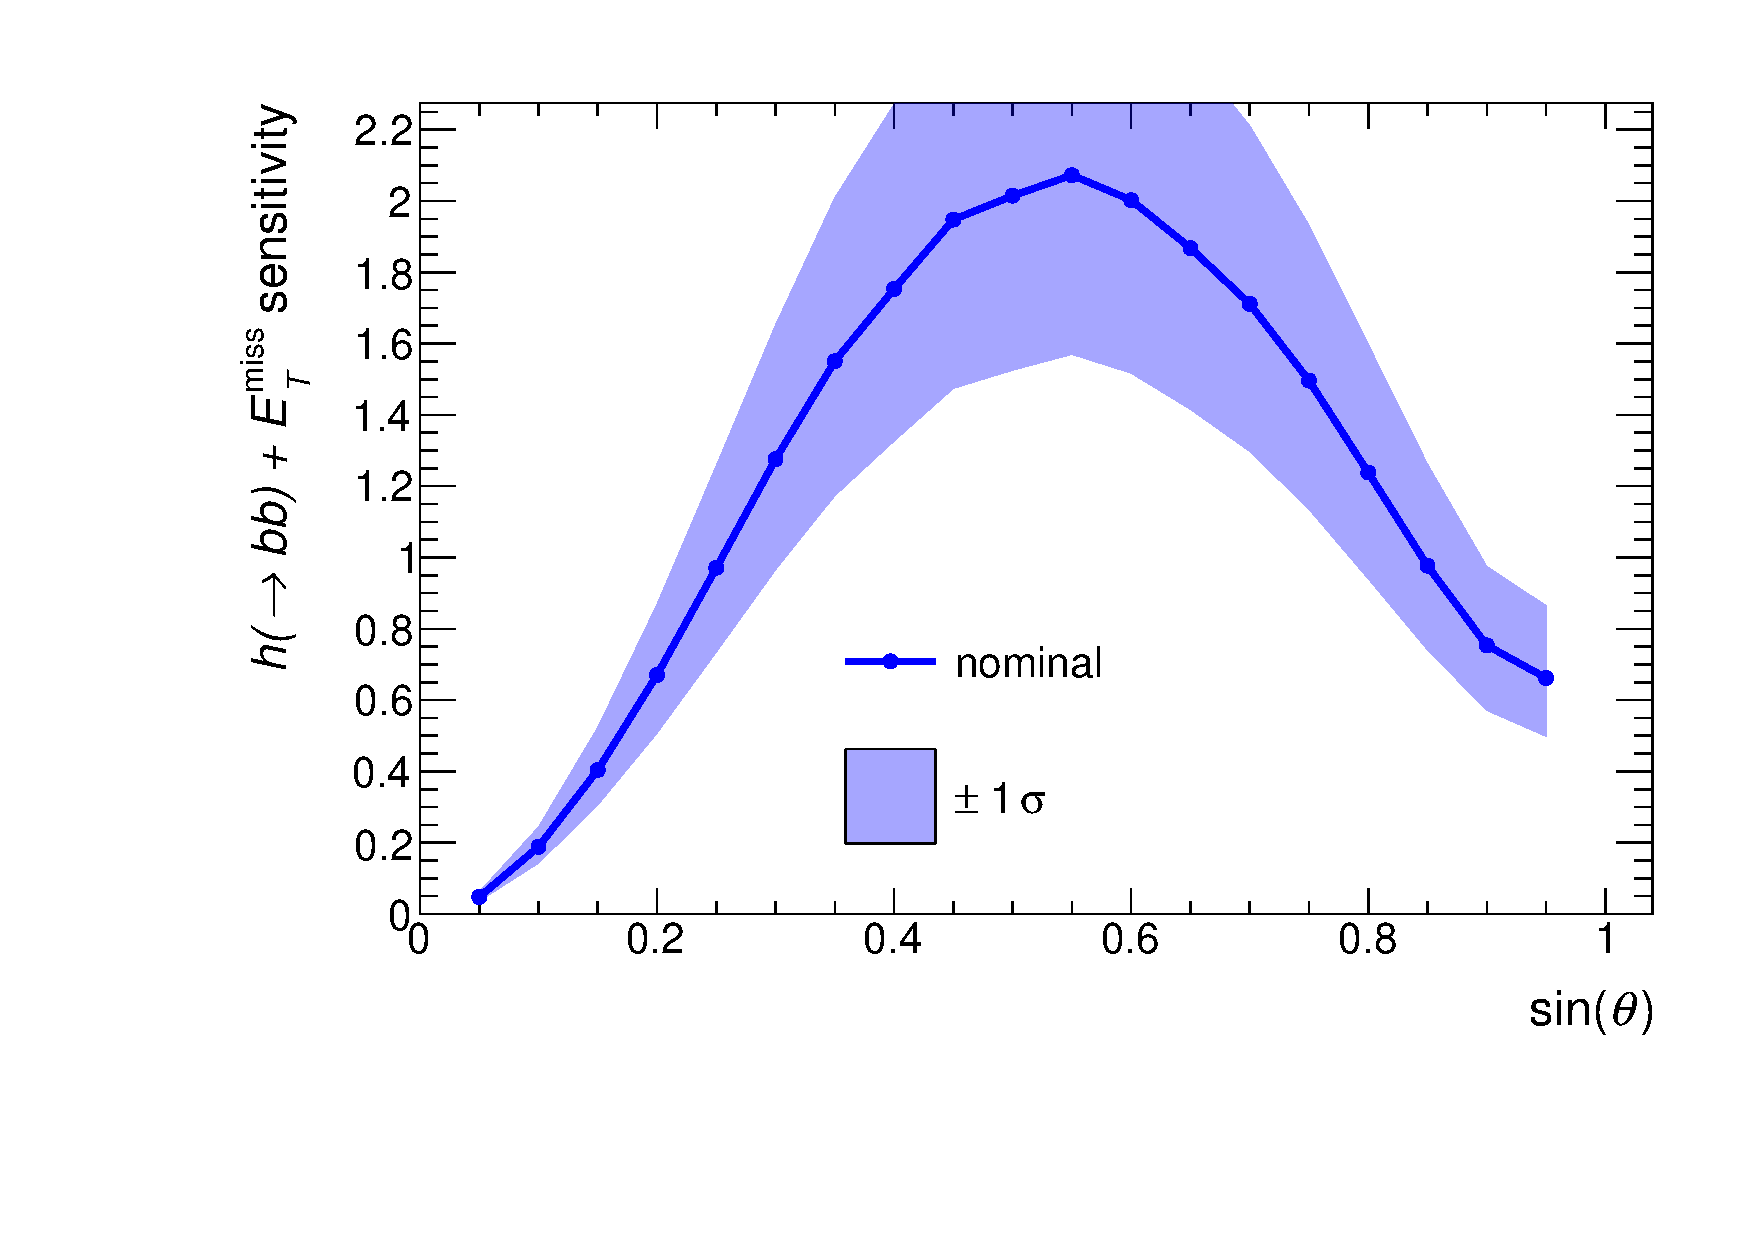
\includegraphics[width=0.49\textwidth]{texinputs/04_grid/figures/monoHbb_sinp_scan_1_sensi_1D.pdf}
%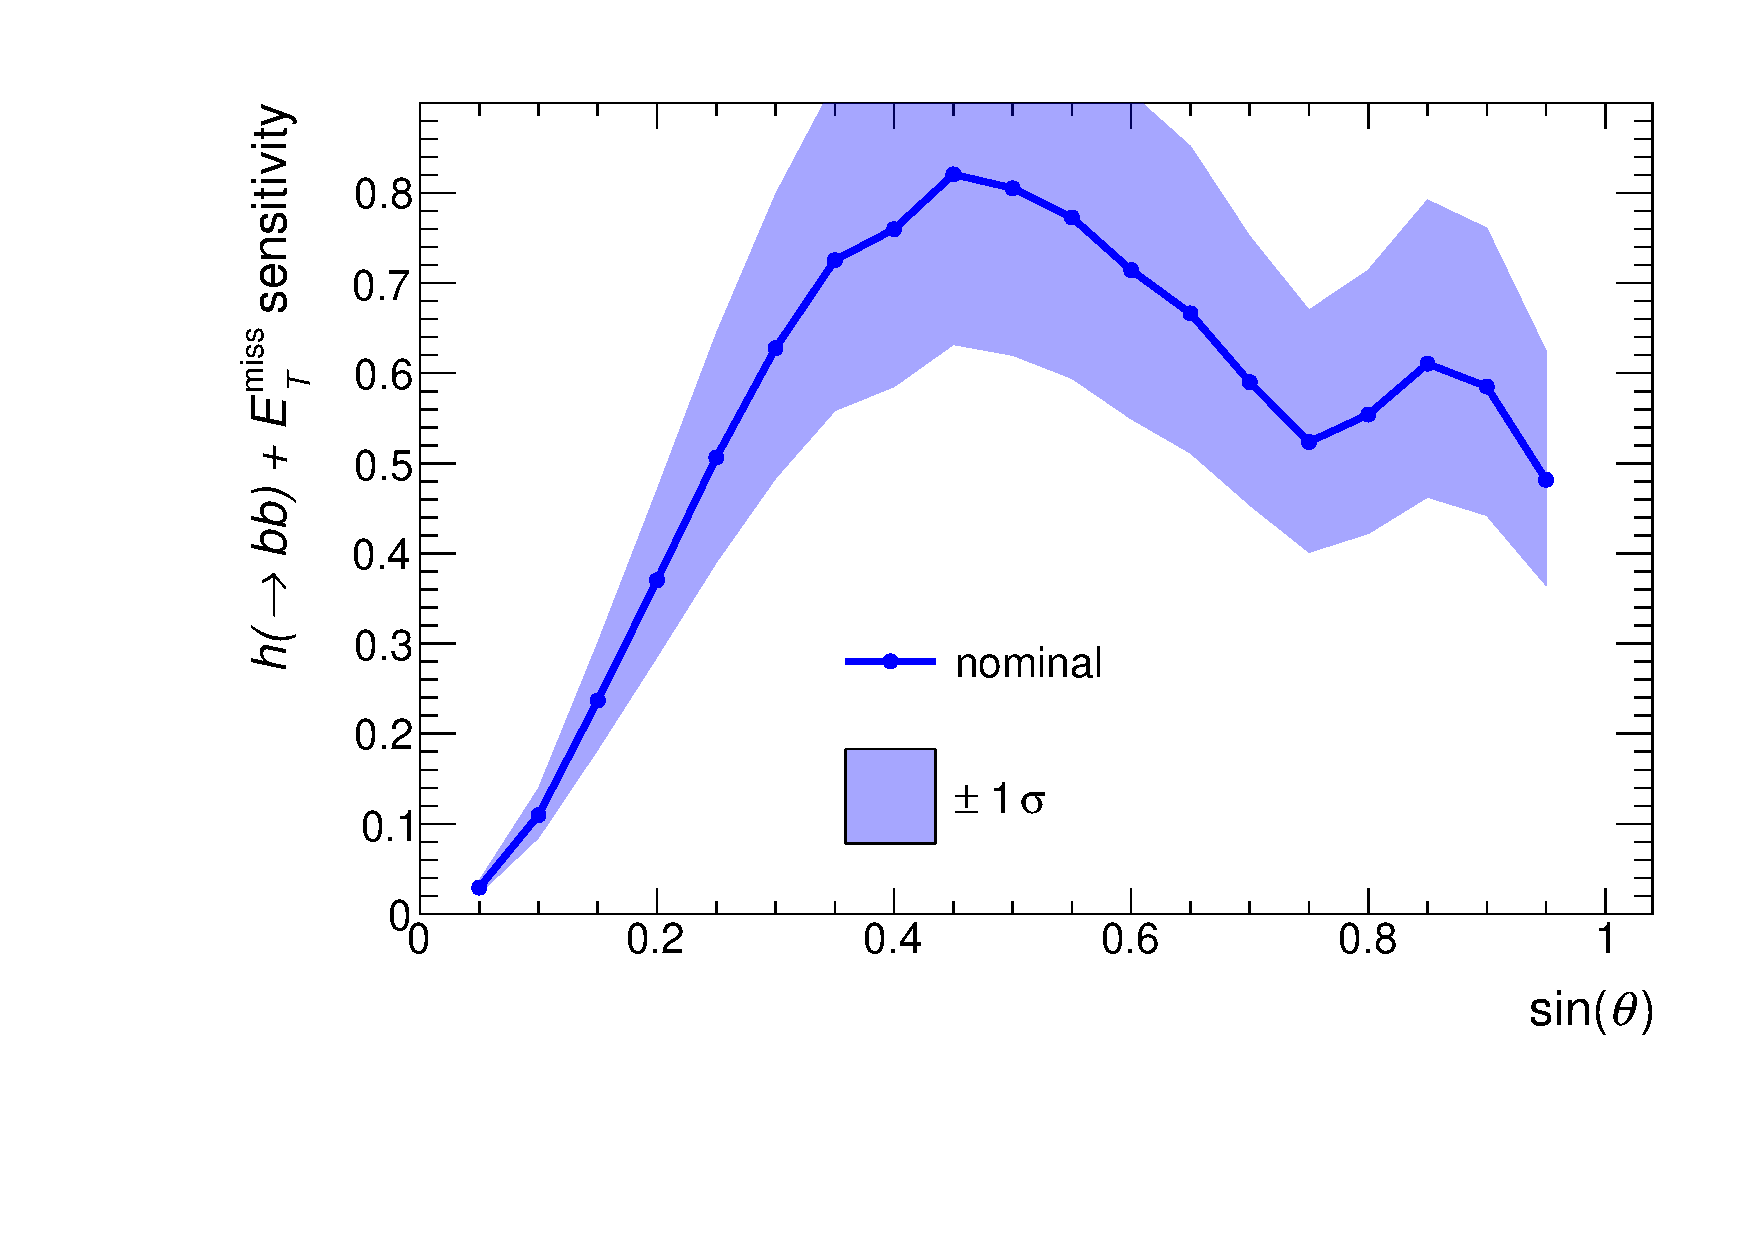
\includegraphics[width=0.49\textwidth]{texinputs/04_grid/figures/monoHbb_sinp_scan_2_sensi_1D.pdf}
%\caption[Sensitivity to $h\to bb + \MET$ signals with different $\sinp$, summed across $\MET$ bins]
%{
%Sum over all $\MET$-bins of the estimated signal sensitivity to $h\to bb + \MET$ events as a function of the pseudoscalar mixing parameter $\sinp$, for $\ma = 200~\GeV$ and $\mH=\mHc=\mA = 600$~GeV~(left) as well as $\ma = 350~\GeV$ and $\mH=\mHc=\mA = 1000$~GeV~(right). The remaining parameters take the values
%$\mDM = 10 $ GeV$, \tanb = 1,$ and $ \lap1 = \lap2 = \lam3 = 3 $.
%The sensitivity, defined in \autoref{eq:monoHbb_sensi}, as well as the uncertainty on the sensitivity (shaded blue) 
% are based on the limits with reduced model dependence from Ref.~\cite{Aaboud:2017yqz} and the uncertainties described therein. 
%}
%\label{fig:monoHbb_sensi_full_sinp}
%\end{figure}




%\begin{figure}[tbp]
%\centering
%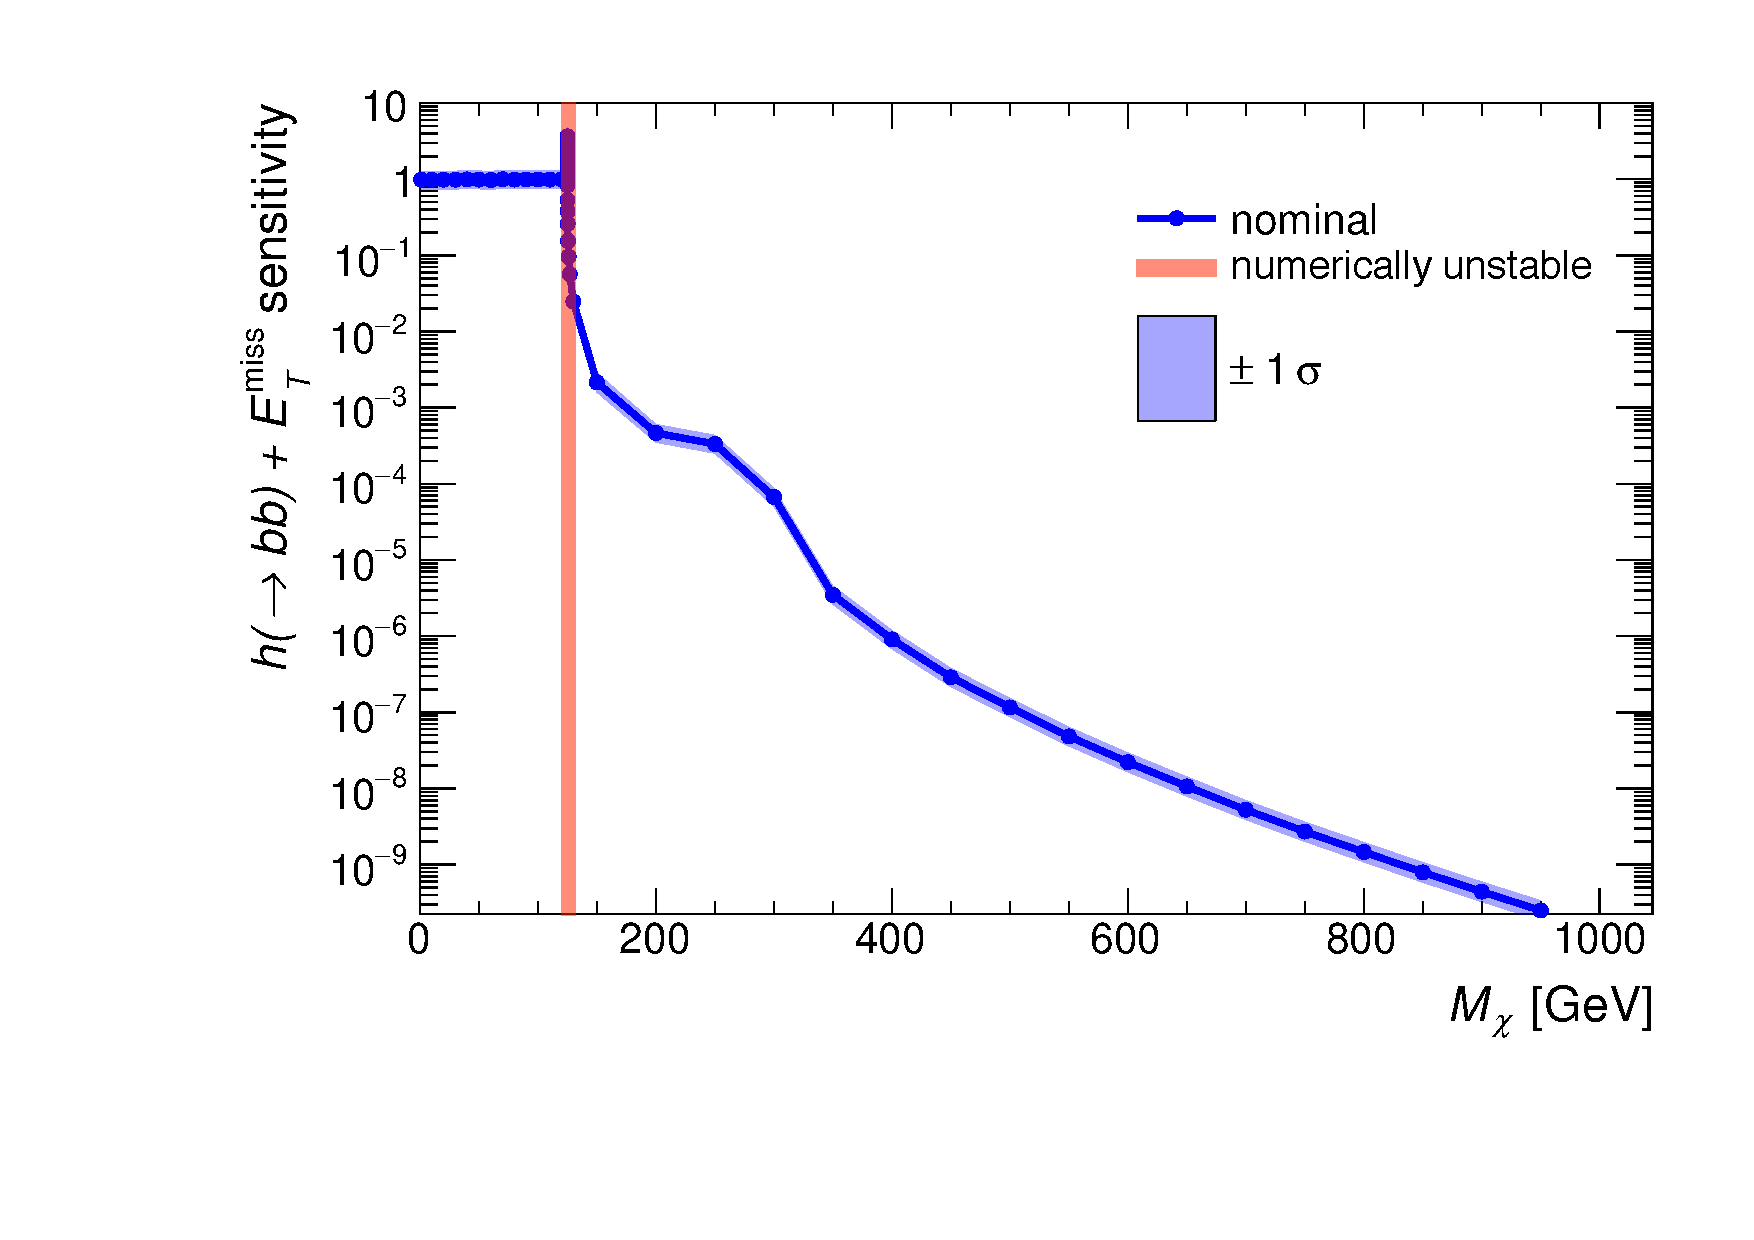
\includegraphics[width=0.7\textwidth]{texinputs/04_grid/figures/monoHbb_sensi_mDM_scan.pdf}
%\caption[Sensitivity to $h\to bb + \MET$ signals with different $\mDM$, summed across $\MET$ bins]
%{
%Sum over all $\MET$-bins of the estimated signal sensitivity to $h\to bb + \MET$ events as a function of the DM mass $\mDM$. 
%The sensitivity, defined in \autoref{eq:monoHbb_sensi}, as well as the uncertainty on the sensitivity (shaded blue)
%are based on the limits with reduced model dependence from Ref.~\cite{Aaboud:2017yqz} and the uncertainties described therein. 
%The remaining parameters take the values
%$ \ma = 250 $ GeV$, \mH=\mHc=\mA = 600$ GeV, $ \sinp = 0.35, \tanb = 1,$ and $ \lap1 = \lap2 = \lam3 = 3 $. 
%The sensitivity is constant below $\mDM < \ma/2$, and rapidly drops for $\mDM > \ma/2$. The sensitivity is resonantly enhanced for $\mDM = \ma/2$.}
%\label{fig:monoHbb_sensi_full_mDM}
%\end{figure}

%The sensitivity estimate of ATLAS and CMS to the \hdma scenario through the \monohbb signature is based on limits on anomalous production of 125 GeV Higgs bosons in association with \met with minimal model dependence~\cite{Aaboud:2017yqz}. The limits are translated to parton level and compared to parton-level simulations of the \hdma scenario for the sensitivity estimate. This approach avoids the simulation of the detector response, which requires a significant amount of computing resources, and more iterations and refinements of the signal grid can be performed. 

%The limits with minimal model dependence are provided in terms of the detector-level cross section of $\monohbb$ events $\sigma_{i}^{\mathrm{obs},\,\monohbb}$ as a function of \met in four bins $i=1,...4$~\cite{Aaboud:2017yqz}. 
%To compare these values to the simulation results at parton level, 
%an estimate of the detection efficiency $\varepsilon$ times the kinematic acceptance $\mathcal{A}$ of the event selections of the analysis is used for each of the four $\MET$ bins.
%%This estimate is provided as one $(\mathcal{A\times\varepsilon})$ value for each of the four $\MET$ bins. 
%Thus, the $(\mathcal{A}\times\varepsilon)_i$ figure represents the minimum probability
%that an event generated at parton level in a given $\MET$ bin $i$ is reconstructed in that same $\MET$ bin and passes all analysis selections.
%%The limits with minimal model dependence are provided separately for each of the four $\MET$ bins used in \cite{Aaboud:2017yqz}.
%%Thus, the simulated evebts are binned into those bins (\autoref{fig:monoHbb_xsec_bins_mA_ma}).
%Consequently, the cross section for \hdm production in the \hdma scenario at parton level $\sigma_{i}^{\mathrm{parton},\,\hdm}$ is calculated in the same $\MET$ bins as used in the \monohbb search. This starting point is shown in \autoref{fig:monoHbb_xsec_bins_mA_ma} using the scan in $(\mA,\ma)$ as a representative example. 
%In the next step, the sensitivity $\sens_i$ for each of the \met bins $i=1,...4$ is calculated as
%\begin{equation}
%\label{eq:monoHbb_sensi_i}
%\sens_i \equiv \frac{\sigma_{i}^{\mathrm{parton},\,\hdm} \times \mathcal{B}^{\mathrm{SM},\,h\to bb} \times (\mathcal{A\times\varepsilon})_{i} }
%{\sigma_{i}^{\mathrm{obs},\,\monohbb}}\,,
%\end{equation}
%where $\mathcal{B}^{\mathrm{SM},\,h\to bb}$ is the $h\to bb$ branching ratio predicted by the SM for the 125~GeV Higgs boson. A representative example for this step is given in \autoref{fig:monoHbb_sensi_bins_mA_ma} for the scan in $(\mA,\ma)$.  A particular point in the $(\mA,\ma)$ parameter parameter space is excluded if $\sens_i \geq 1$. Finally, to obtain a single estimate for the total sensitivity $\senstot$ using all four $\MET$ bins, their individual contributions from \autoref{eq:monoHbb_sensi_i} are summed over\footnote{
%This choice is made because the individual per-bin sensitivities follow a logarithmic metric, and because a model will typically populate several \met bins at a time. This implies that there could be models where $\sens_i<1$ in every bin, yet the sum from \autoref{eq:monoHbb_sensi} is $>1$.
%Therefore, for a rigorous exclusion of a model based on the limits with minimal model dependence, the preferred approach would be to consider only the most sensitive bin for the exclusion.
%}:
%\begin{equation}
%\label{eq:monoHbb_sensi}
%\senstot \equiv \sum_{i\in\met~\mathrm{bins}} \sens_i\,.
%\end{equation}
%The resulting $\senstot$ is shown in \autoref{fig:monoHbb_sensi_full_mA_ma} for the example of the $(\mA,\ma)$ scan.


%The scan of the sensitivity in the sense of \autoref{eq:monoHbb_sensi} in the $(\ma,\mA)$ plane is shown in \autoref{fig:monoHbb_sensi_full_mA_ma}.
%The sensitivity decreases with increasing $\mA = \mH = \mHc$ for $\mA \geq 1$~TeV because the fraction of resonant signal events drops. 
%This drop is caused by increasingly large $\Gamma_A$, 
%which allows for an increasing fraction of non-resonant signal events, driven by events with very off-shell $A$. % ref ggF-> A -> ah feynman graph
%%Non-resonant signal events have soft $\MET$ and thus the search is less sensitive to them, since the minimum accepted $\MET$ is $\MET \geq 150$ GeV.
%Near the mass diagonal $\ma = \mA$, there is little to no sensitivity. 
%This is because the Jacobian peak moves to low $\MET$ for a small mass splitting $|\mA - \ma|$
%(\autoref{eq:monoH_peak_met}, \autoref{fig:monoHbb_mA_scan_met}, and \autoref{fig:monoHbb_ma_scan_met}).
%Beyond this, the coupling $g_{Aah}$ is small when all Higgs bosons are nearly degenerate in mass, cf.~Equation~4.12 in Ref.~\cite{Bauer:2017ota}, %ref to eq.in theory part(?)
%resulting in a small total cross section and therefore further decrease in sensitivity.
%The sensitivity above the mass diagonal, $\mA > \ma$, is larger than below the mass diagonal.
%Two parameter choices cause this asymmetry:
%\begin{enumerate}
%\item 
%$\mA = \mH = \mHc$, i.e., the neutral and charged $CP$-even scalars have low masses below the diagonal, but high masses above it, introducing an asymmetry.
%Another effect can be seen in \autoref{fig:monoHbb_mH_scan_met}: values of  $\mH = \mHc$ below the mass of the higher-mass pseudoscalar (in this case $A$)
%give a reduced total cross section and a lower fraction of resonant signal events. Both effects reduce sensitivity;
%\item 
%$\sinp = 0.35 \neq 1/\sqrt{2}$, i.e. the mixing between the pseudoscalars $A$ and $a$ is asymmetric. 
%$A$ couples more strongly to SM particles than $a$, and vice versa for the couplings to the DM fermion $\chi$.
%So the situation below the diagonal corresponds to the case of $\sinp = \sqrt{1-0.35^2} \approx 0.938$ and $\mA > \ma$. 
%As can be seen in \autoref{fig:monoHbb_sinp_scan_mA600_ma200_met},
%this \sinp configuration has a higher fraction of non-resonant signal events with low \met, and correspondingly a lower sensitivity is found in \autoref{fig:monoHbb_sensi_full_sinp}.
%\end{enumerate}
%
%The scan of the sensitivity in the  $(\ma,\tanb)$ plane is shown in  \autoref{fig:monoHbb_sensi_full_ma_tanb}. 
%At very low $\tanb$, the Yukawa coupling to top quarks is large, and most of the signal events come from non-resonant processes, as can be seen from \autoref{fig:monoHbb_tanb_scan_met}. % ref to tanb met scan
%The non-resonant processes are characterised by soft $\MET$, which lowers the kinematic acceptance and reduces the sensitivity of the search.
%For higher $\tanb$, the fraction of resonant events increases due to the reduced top Yukawa coupling, resulting in an increase of sensitivity.
%However, reducing the top Yukawa coupling also reduces the total production cross section. 
%This effect is sub-dominant below $\tanb \approx 1.2$, and the sensitivity increases with $\tanb$. 
%But above $\tanb \approx 1.2$, the sensitivity loss due to reduced cross section outpaces the sensitivity gain due to a more resonant signal.
%Overall, the search gets less sensitive with increasing $\tanb$ above $\tanb \approx 1.2$.
%At very high $\tanb$ ($\geq 10$), this trend is reversed again because the $\tanb$ enhancement\footnote{The \hdma scenario assumes a Yukawa sector of type II.} of the 
%coupling to $b$-quarks compensates for the small $b$-quark mass.
%At this point $bb$ initiated processes start to dominate the production cross section and drive the increase in sensitivity.
%
%The sensitivity to models with varying $\sinp$ is shown in \autoref{fig:monoHbb_sensi_full_sinp}.
%The sensitivity vanishes at $\sinp=0$ and $\sinp=1$, since those values correspond to no mixing between $A$ and $a$, and thus no connection between the SM and the dark sector. 
%For its intermediate values, the $\sinp$ parameter influences the couplings of the pseudoscalars to DM as well as to SM fermions, 
%and also the coupling strength of trilinear scalar vertices such as $g_{Aah}$~\cite{Bauer:2017ota}. 
%Increasing the couplings increases the total cross section. 
%However, increasing some couplings can also increase $\Gamma_A$ and thereby decrease the resonant fraction of signal events and the sensitivity.
%The upshot of this is that there can be more than one local maximum in the sensitivity curve, as shown the right panel of~\autoref{fig:monoHbb_sensi_full_sinp}. 
%The precise dependence of the sensitivity on \sinp depends on the precise interplay of the couplings.
%Because the couplings depend on all other model parameters including all the Higgs masses, 
%tuning the $\sinp$ of a parameter scan to the sensitivity in a single point can lead to sub-optimal sensitivity in other points.
%
%The sensitivity to models with varying $\mDM$ is shown in  \autoref{fig:monoHbb_sensi_full_mDM}.
%Below the threshold of $\mDM < \ma/2$, the sensitivity is constant since the $\MET$ distribution and the total signal cross section remain invariant, as demonstrated in \autoref{fig:monoHbb_mDM_scan_met}.
%At threshold, the sensitivity is enhanced because the partial width for $ a \to \chi \chi $ is enhanced, 
%increasing the signal cross section.
%Above threshold, the sensitivity drops rapidly because $\mDM > \ma/2$ requires an off-shell $a^{\star} \to \chi\chi$ decay, which is strongly suppressed by the typically  narrow width of $a$. 
%The width of $a$ is substantially reduced once $a\to \chi \chi$ is kinematically inaccessible, 
%as $\Gamma_{a\to \chi \chi}$ is a large contribution to the total width of $a$ for $\mDM \leq \ma/2$ \cite{Bauer:2017ota}.
%There is a slight increase in sensitivity for $\mDM \approx \mA/2$ when the $A\to \chi\chi$ decay hits its kinematic threshold, yet the absolute sensitivity remains negligible.


\FloatBarrier
\subsubsection{Studies of the mono-Z (leptonic) signature}
Mono-Z analyses use events with a Z boson recoiling symmetrically against \MET to detect the production of invisible particles.
In previous LHC analyses~\cite{Aaboud:2017bja,Sirunyan:2017qfc}, the DM interpretations of the analysis results have focused on either invisible decays of the SM-like Higgs bosons or topologies where the Z boson is produced as initial-state radiation (ISR) off a quark. The ISR-based topologies generically favor radiation of a gluon or photon rather than a massive gauge boson, thus limiting the discovery sensitive of a Z-based approach compared to monojet and mono-photon searches. In contrast, the model studies in this document generates the mono-Z signature dominantly via the all-bosonic H-a-Z vertex, which can lead to enhancements of the mono-Z sensitivity compared to jet and photon signature. In this section, the behavior and experimental accessibility of the model in Z+\MET events is studied.

\paragraph{Technical setup}
Simulated event samples for the leptonic mono-Z signature are produced with Madgraph5\_aMC@NLO version 2.4.3, interfaced with Pythia version 8.2.2.6 for parton showering. The NNPDF3.0 PDF set is used at LO precision with the value of the strong coupling constant set to $\alpha_{S}(M_{Z}) = 0.130$ (NNPDF30\_lo\_as\_0130). A five floavor scheme with a massless b-quark is used.  Only contributions from gluon-gluon initial states and \lp\lm$\chi\overline{\chi}$ final states are considered, where l = e or $\mu$.  For the range of \tanb values studied, the $bb$ initiated ME contribution is negligible.  To increase calculation efficiency diagrams with an intermediate s-channel SM Higgs boson are explicitly rejected (generate g g $>$ xd xd~ l+ l- / h1).


\paragraph{Event selection}
Three consecutive stages of event selection are considered:
\begin{itemize}
\item Inclusive: Lepton \pt and $\eta$ requirements corresponding to the typical experimental trigger acceptance are applied.

\item Preselection: A dilepton candidate with an invariant mass in a window around the Z mass is required, and a minimum transverse momentum of the $\chi\overline{\chi}$ system is required.

\item Final selection: Requirements on the main discriminating variables used in the relevant analyses are added: The angular separation in the transverse plane between the $\chi\overline{\chi}$ and \lp\lm systems $\Delta\Phi(ll,\MET)$, the relative transverse momentum difference between them $|p_{T,ll} - \MET|/p_{T,ll}$ and the angular separation between the leptons $\Delta R(ll)$. Additionally, the \MET requirement is tightened.
\end{itemize}

The exact event selection criteria are listed in Tab.~\ref{tab:monozll_selection}.

\begin{table}
\centering
\caption{Event selection requirements for the analysis of the Mono-Z signature with leptonic Z decays.
        The requirements are inspired to follow those used in typical experimental analyses.}
\begin{tabular}{c | c |r l}
Selection stage & Quantity & Requirement \\\hline


\multirow{ 2}{*}{Inclusive}         & lepton $\left|\eta\right|$                    & $< 2.5$ \\
                                    & leading (trailing) lepton \pt                 & $> 25 (20)$ GeV \\\hline

\multirow{ 2}{*}{Preselection}      & $\left|m_{ll}-m_{Z,\mathrm{nominal}}\right|$  & $< 15$ GeV\\
                                    & \MET                                          & $> 40$ GeV \\\hline

\multirow{ 3}{*}{Final selection}   & $\Delta\Phi(ll,\MET)$                         & $>2.7$\\
                                    &$|p_{T,ll} - \MET|/p_{T,ll}$                   & $<0.4$\\
                                    &  $\Delta R(ll)$                               & $<1.8$\\
                                    &  \MET                                         & $>80$ GeV \\ 
\end{tabular}


\label{tab:monozll_selection}

\end{table}


\paragraph{Cross-sections, kinematic distributions, and acceptances}
The overall cross-sections in the \tanb and mass scans are shown in Fig.~\ref{fig:monoz_ll_xs_inclusive}.
In the mass scan, maximal cross-sections are observed for the region of $\ma < \mA$ for values of $\ma\gtrsim100$ GeV. Towards higher values of both \ma and \mA, the cross-sections fall off, reaching values smaller than $1$ fb at $\ma\approx450$ GeV or $\mA\approx1.1$ TeV. In the $\ma\approx\mA$-region, the cross-section is suppressed by destructive interference. For the region with inverted mass hierarchy $\ma>\mA$, cross-sections of the order of multiple fb are observed, as long as $|\ma-\mA|$ remains sufficiently large.
In the \tanb scan, cross-sections smoothly fall with increasing $\ma$ as well as $\tanb$. Cross-sections are typically larger than 1 fb up to $\tanb\approx5$. The $\ma$ dependence is modulated by the value of \tanb: Crossing the $\ma$ range from $100$ to $400$ GeV, cross-sections are reduced by a factor $\approx7$ for small $\tanb\approx1$, but only a factor $\approx2$ for higher values of $\tanb\approx5$.
In the \sinp scan shown in Figure \ref{fig:monoz_ll_sinp_scan_xsec}, cross sections depends on whether or not the $a \rightarrow \ttbar$ decays are accesible.  
For $\ma < 350$ GeV they are not accesible and cross section strictly increases with \sinp.  For $\ma > 350 \GeV$, the $a \rightarrow \ttbar$ decays become possible causing the cross section to decrease for large values of \sinp.

%For \ma <350 GeV they are not accesible,  and only the heavy scalar's branching fraction to $aZ$ is relevant.  This branching fraction stricly increases with \sinp.  For \ma > 350 \GeV, the branching fraction of $a \rightarrow \chi \chi$ also becomes important, and there is a turnover point were the cross section decreases.

To assess the kinematic behavior of the signal, distributions of kinematic variables most relevant to the Mono-Z signature are studied as a function of the model parameters.

The distribution of the invariant masses of the dilepton and $\chi\chi$ systems are shown in Fig.~\ref{fig:monoz_kin_inclusive}. Independent of the parameters, the dilepton mass spectrum is centered at the Z peak, without any nonresonant contribution. The $M_{\chi\chi}$ distribution illustrates the signal contributions from different diagrams. For $\mA>\ma$, DM is dominantly produced from on-shell $a$ boson production. In the inverted mass region $\mA<\ma$, the situation is reversed, and $H$ diagrams dominate.

After applying the preselection requirements, scans of the model parameters are performed.  For this paper a subset of models are studied where \mA is degenerate with \mH.  Similar to mono-h, for mono-Z in the region $\mA>\ma$a resonantly produced heavy scalar, $H$, decaying to $aZ$ produces a characteristic Jacobian peak in the \MET distribution.  The location of the peak depends on \mH and \ma as given by equation \ref{monoZ_jacobian_peak}, and its width generally increases with values of  $\ma$ and $\mA$.  

\begin{align}
E^{\mathrm{miss},max}_T \approx \frac{\sqrt{\left(\mH^2 -\ma^2 -M_{Z}^2\right)^2 - 4 \ma^2 M_{Z}^2}}{2\mH}\,.
\label{eq:monoZ_jacobian_peak}
\end{align}

Figure \ref{fig:monoz_ll_mA_scan} shows the Jacobian peaks for increasing values of \mH and fixed \ma.  Significant portions of the spectrum are situated at relatively high boosts ($\MET>\unit[200]{GeV}$), which is more easily accessible experimentally.  This behavior is contrasted by the distributions in the inverted mass regions, which have nearly no distinct features and are mainly located at low mediator \pt. For $\mA\approx\ma+m_{Z}$, both the a and Z bosons are produced approximately at rest, leading to an event population with overall low boost. These qualitative trends are consistent with the distributions of the other main selection variables shown in Fig.~\ref{fig:monoz_kin_presel}.

The \tanb and \sinp parameters have minimal effect on the kinematic distributions (Fig.~\ref{fig:monoz_kin_tanb_sintheta}).  For small values of $\tanb$ there is a slight softening and broadening of the \MET distribution due to the increased contribution from non-resonant $z+a$ production.

For the DM mass, in the region where $\mDM < \frac{\ma}{2}$, \mDM has no effect on cross section or kinematic distributions.  In the off-shell region where  $\mDM > \frac{\ma}{2}$ cross section steeply drops and the \MET distribution becomes less structured.


%After applying the preselection requirements, the distributions of kinematic variables are shown in Fig.~\ref{fig:monoz_kin_presel}. 
%In the region of $\mA>\ma$, distinct Jacobian peaks are visible in the distributions of the mediator \pt, the width of which generally increases with values of $\ma$ and $\mA$. 


Finally, the distributions of the $\MET$ and $\MT$ variables after final selection are shown in Fig.~\ref{fig:monoz_kin_final}. Traditionally, the Mono-Z search has relied on the $\MET$ distribution for signal extraction. While the presence of the Jacobian peak structure in the distribution facilitates signal-background separation, it may be beneficial to also consider the $\MT$ distribution. Although only transverse information is available, the resonant structure of the signal is significantly enhanced in the $\MT$ variable, which may enhance the sensitivity of a specialized search strategy.

Acceptances for the mass and \tanb scans are shown in Figures \ref{fig:monoz_ll_acceptance} and \ref{fig:monoz_ll_tanbma_acceptance}.  
In the mass scan, for points where the Jacobian peak is below the analysis's \MET cut, from $\ma = 100$ $\mA = 200$ to $\ma = 300$ $\mA = 400$, 
acceptance drops sharply approaching zero.  Above this region, acceptance levels are grouped into bands for fixed values of $\mA-\ma$. 
With increasing $\mA-\ma$ acceptances increases, gradually plateauing to a maximum value of 50\%.  In the inverted mass region, 
acceptances are generally lower than the rest of the mass scan, but for light values of \ma can reach values as large as 30\%.
In the \tanb scan, acceptances are largely independent of \tanb and constant for equal values of \ma.  For small values of \tanb and
$\ma < 350$ \GeV  there is slight drop in the acceptance caused by the softer \MET distribution from non-resonant decays.  


\paragraph{Expected significance}

The expected sensitivity of the Mono-Z(ll) channel to 2HDM+a models is approximated using generator level signal samples and background estimates from recent $Z(\ell \ell) + \MET$ searches of 36.1 \ifb of data \cite{Aaboud:2017bja}.  For signal events a reconstruction efficiency of 75\% is assumed, and to be consistent with the background estimates, the same selection cuts as \cite{Aaboud:2017bja} are used.  Signal and background are binned in \MET and a conservative 20\% background systematic on the background is assumed for $\MET < 120$ \GeV and 10\% above.

Total significance is defined as the per bin significances summed in quadrature.

\begin{equation}
\mathcal{S} = \sqrt{\sum_{bin} (Z^\prime_{bin})^2}
\end{equation}

Following the Asimov approximation, expected significance for individual bins is calculated as the Poisson ratio of likelihoods modified to incorporate  systematic uncertainties on the background  \cite{Cowan:2012}:  
%(\ref{eq:significance_wsyst})

\begin{equation}
\label{eq:significance_wsyst}
Z^\prime_{bin} = \sqrt{ 2 \cdot \bigg( (s+b) \ln[\frac{ (s+b) (b+\sigma_b^2) } {b^2 + (s+b) \sigma_b^2} ]- \frac{b^2}{\sigma_b^2} \ln[1 + \frac{\sigma_b^2 s}{b(b+\sigma_b^2)} ] \bigg) }
\end{equation}

This metric has the advantage that it accounts for systematic uncertainties and is valid even for $s$ not $\ll b$.  Expected significances are shown in Figure \ref{fig:expected_significance_monozll}, with regions the ATLAS and CMS detectors should be sensitive to, greater than 2, highlighted.

%\begin{equation}
%\label{eq:significance}
%Z = \sqrt{2 \bigg( (s+b) \ln{1 + \frac{s}{b}} - S \bigg) }
%\end{equation}


\paragraph{Conclusions} The Mono-Z(ll) provides experimental coverage of the pseudoscalar 2HDM model for a broad part of the parameter space. The light pseudoscalar \a can be probed up to mass values of $\approx\unit[350]{GeV}$, depending on the choice of other parameters. The Mono-Z is sensitive mostly in the region of low values of $\tanb<4$.

\begin{figure}
\centering
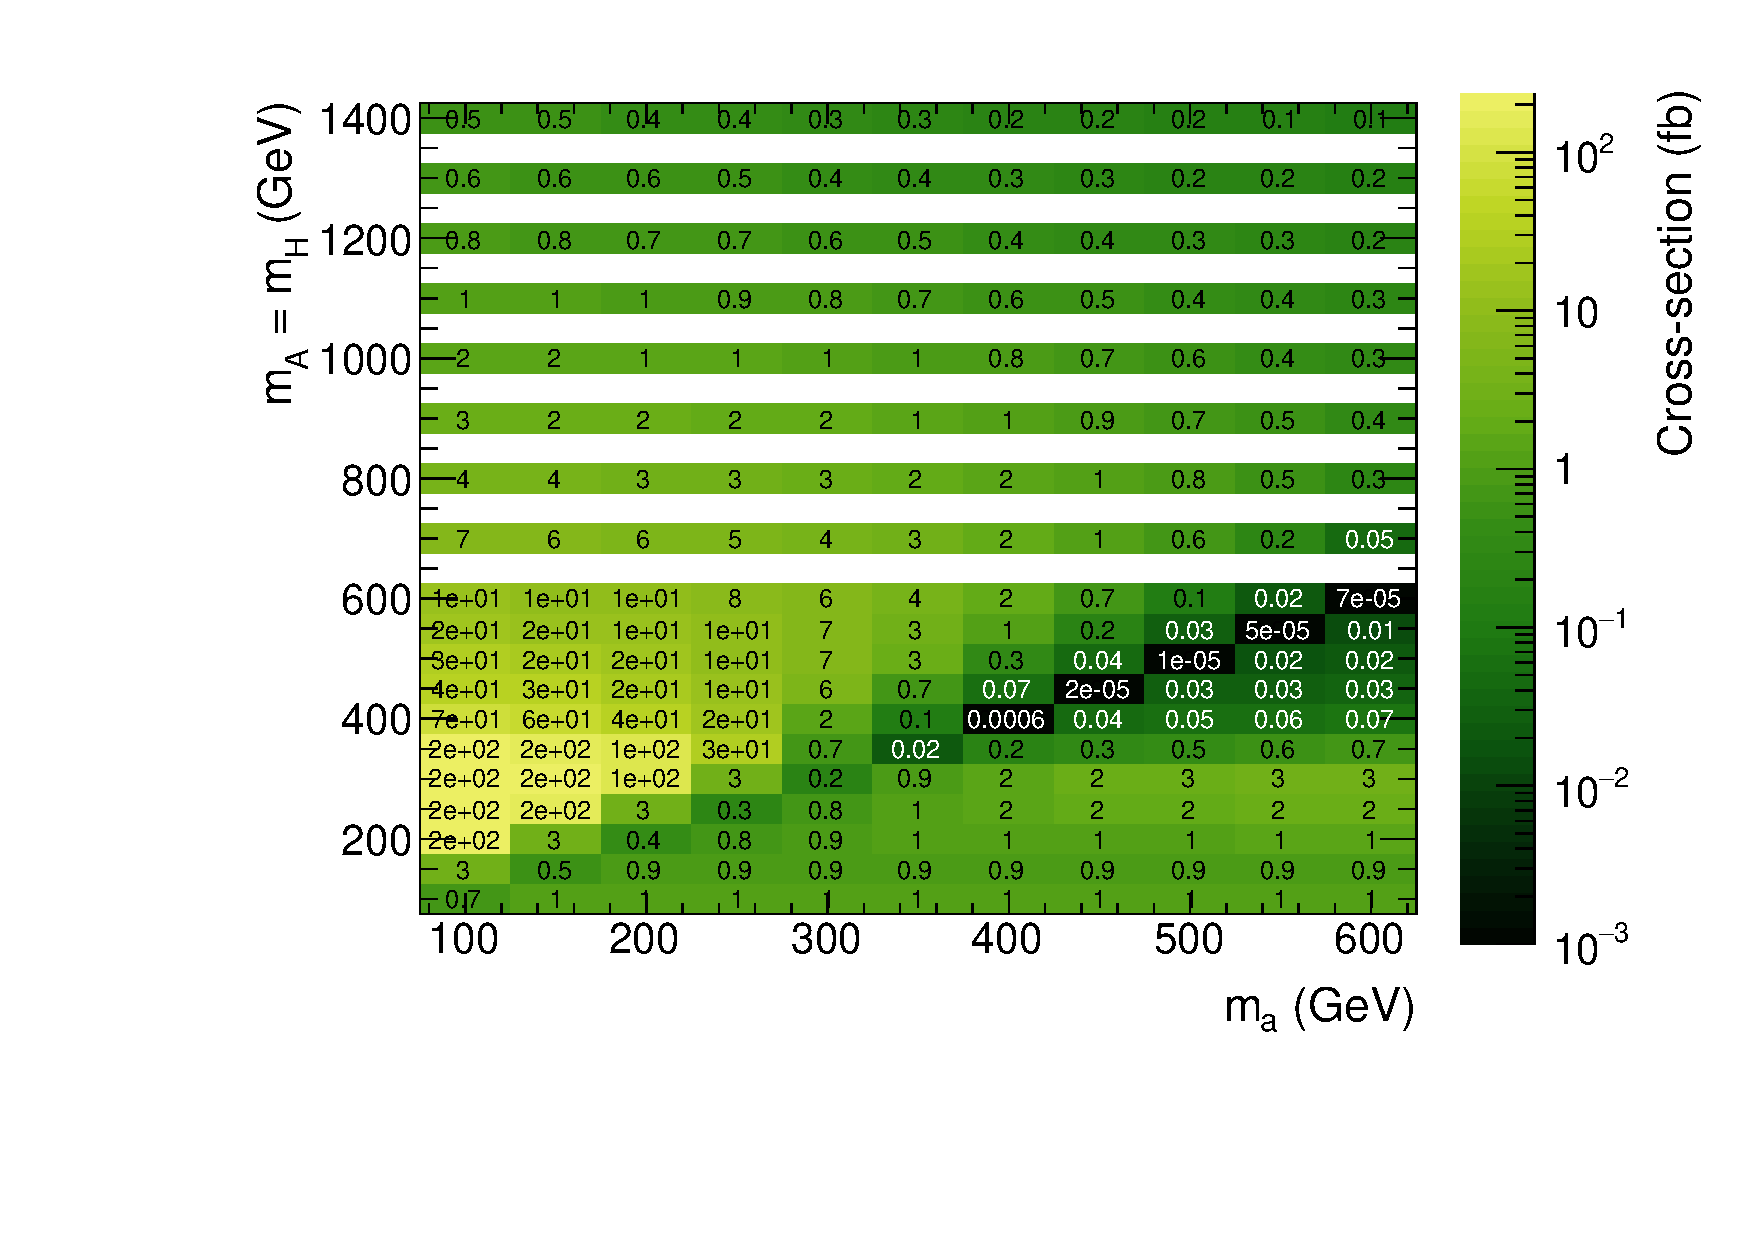
\includegraphics[width=0.8\textwidth]{texinputs/04_grid/figures/monoz/leptonic/xs_2d_inclusive_26300.pdf}
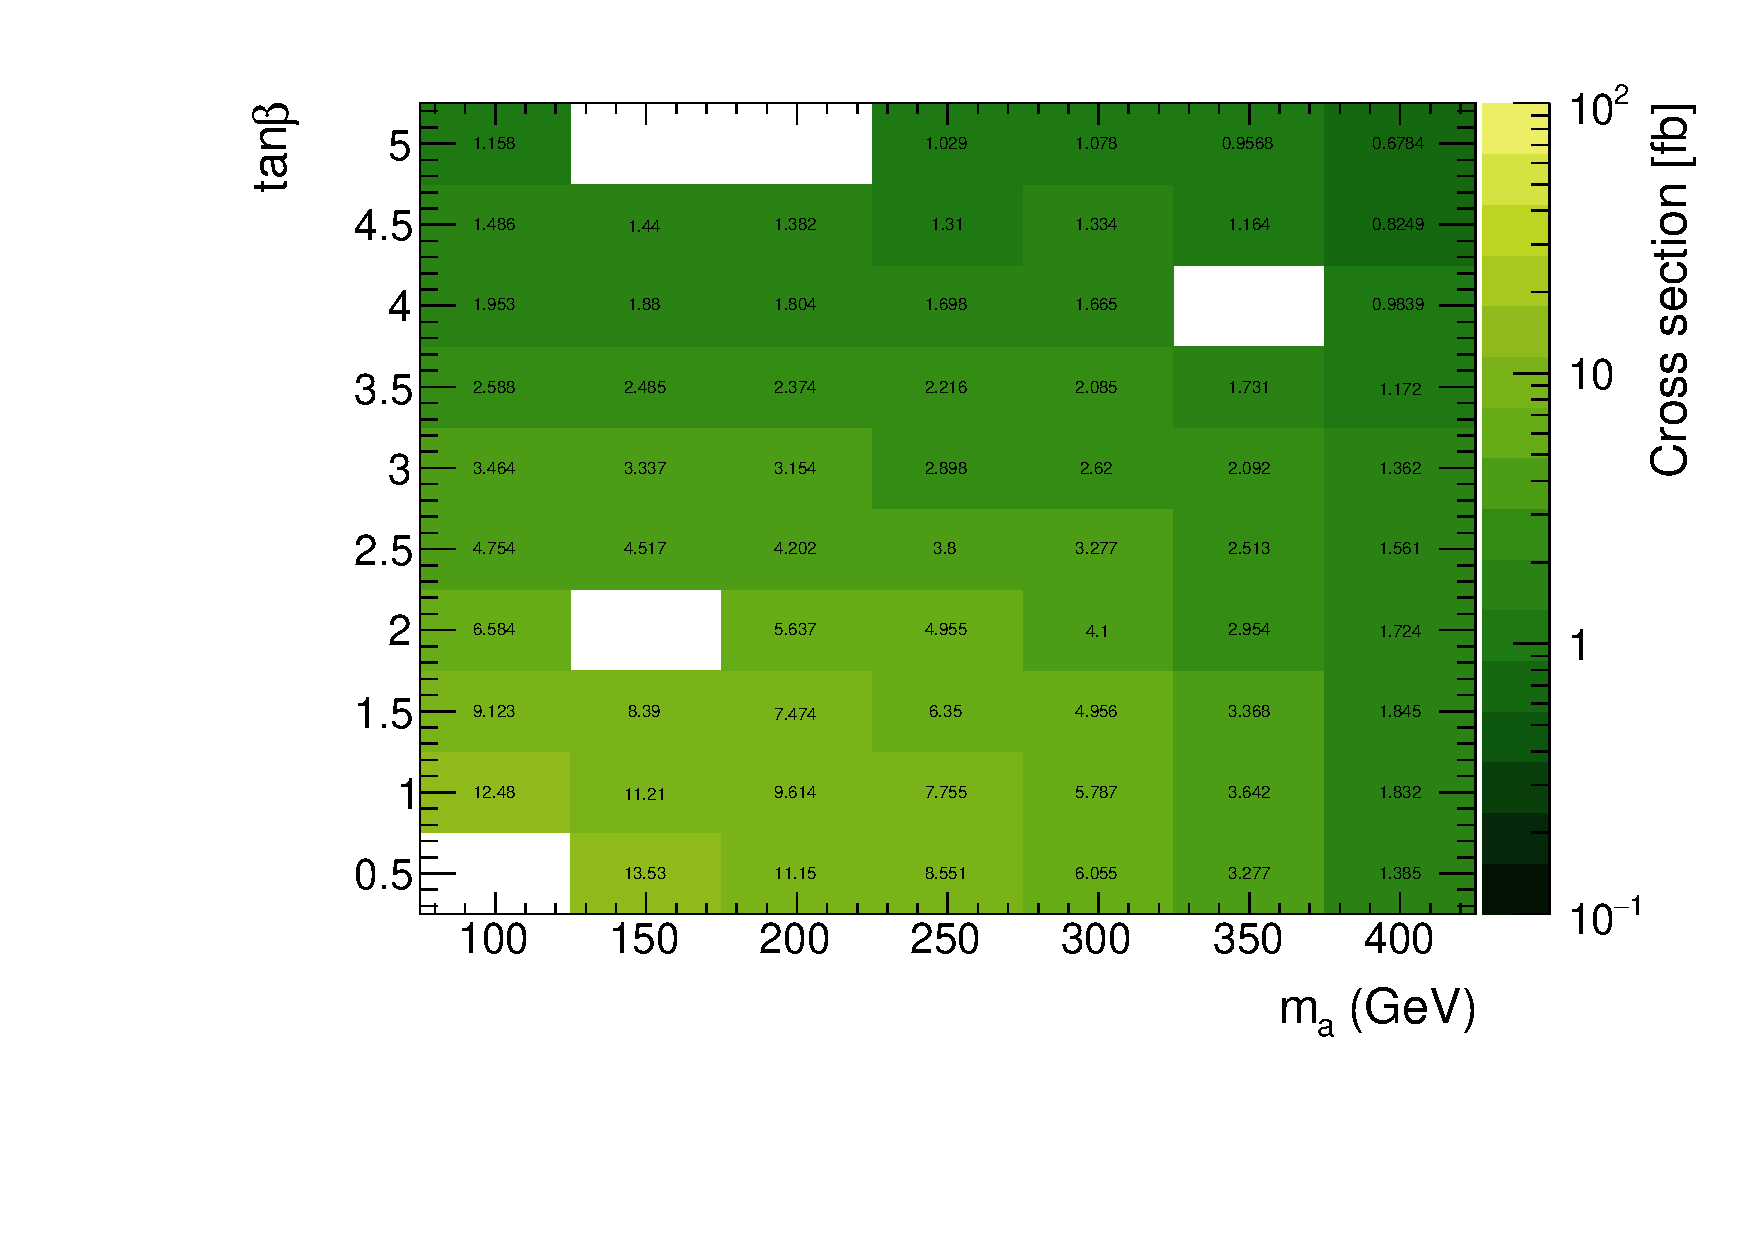
\includegraphics[width=0.8\textwidth]{texinputs/04_grid/figures/monoz/leptonic/tanbma_xsec_ll.pdf}
\caption{Inclusive cross-sections for $pp\rightarrow \lp\lm\chi\overline{\chi}$ in the \ma-\mA (top) and \ma-\tanb scans (bottom).}
\label{fig:monoz_ll_xs_inclusive}
\end{figure}


\begin{figure}
\centering
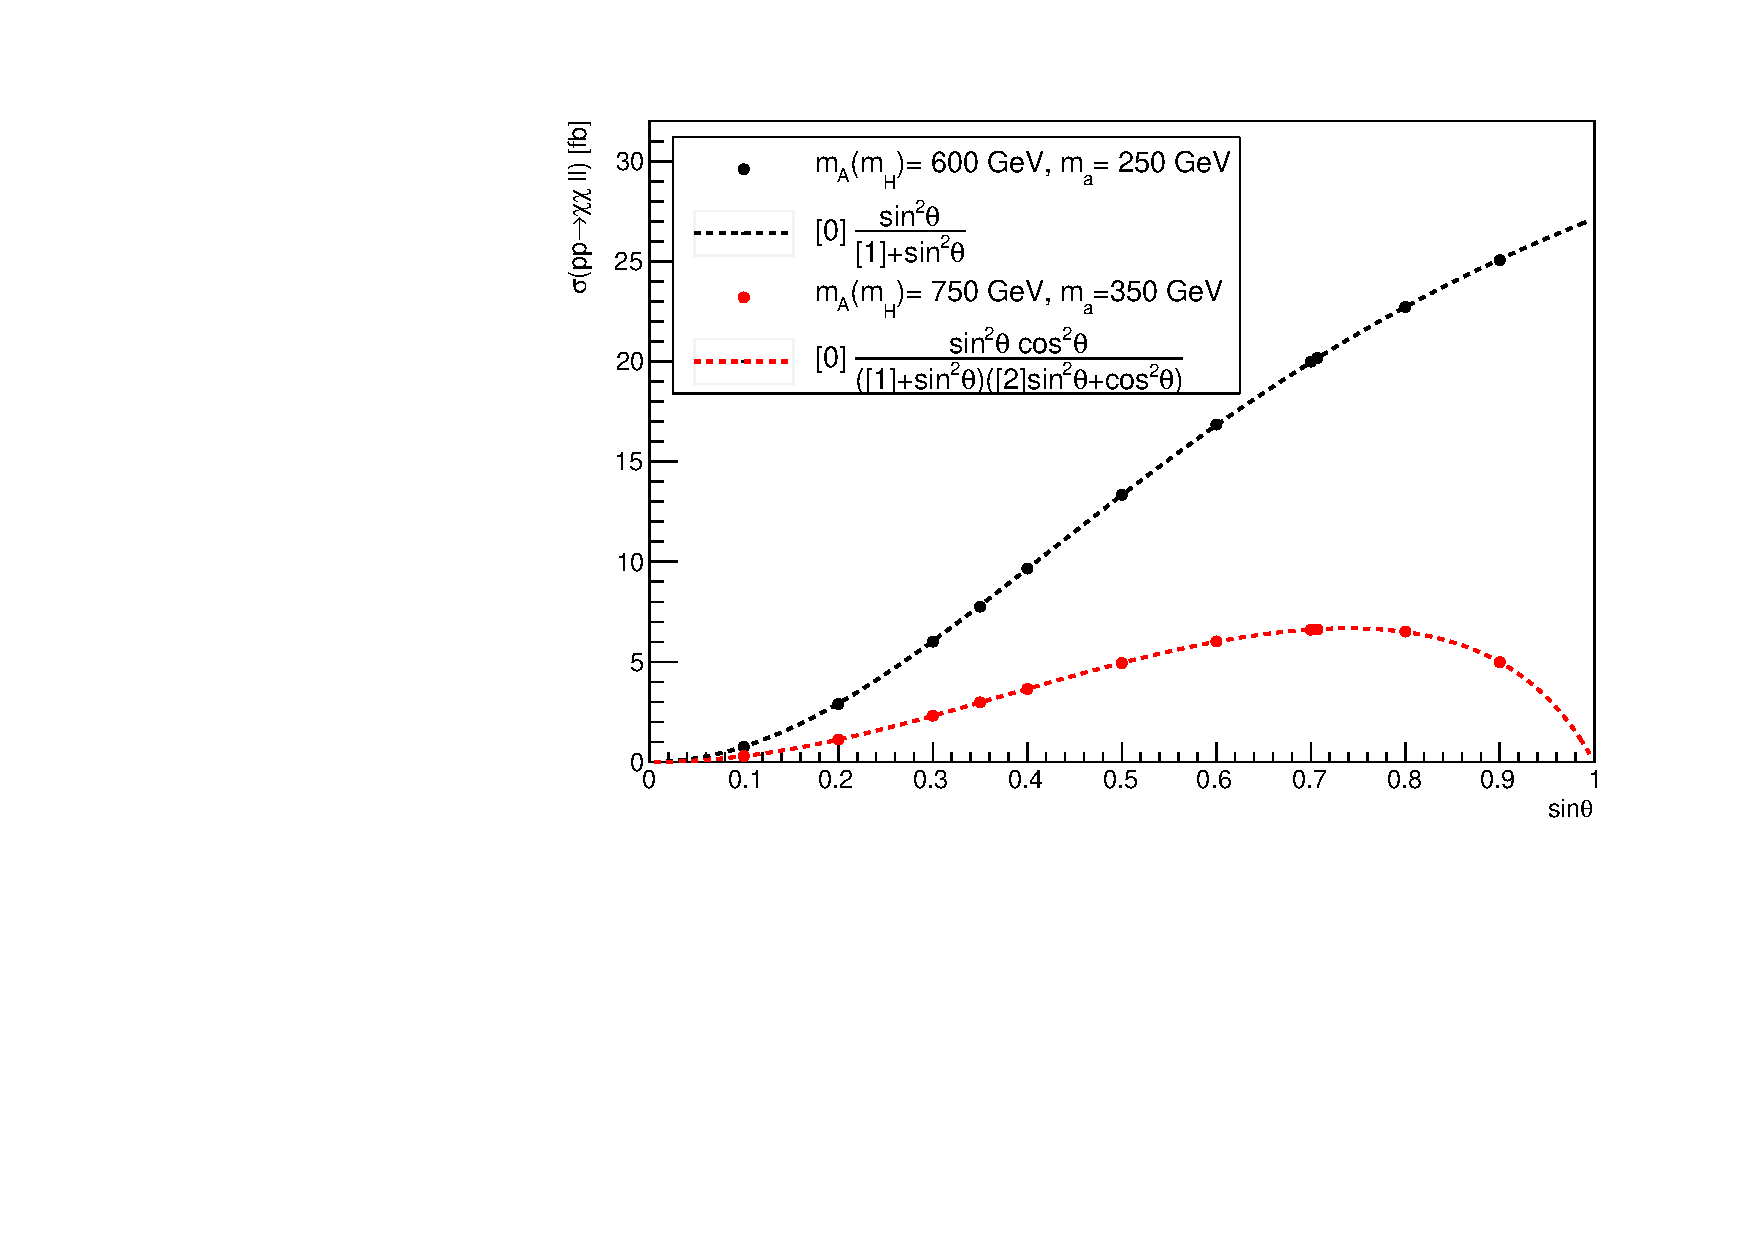
\includegraphics[width=0.6\textwidth]{texinputs/04_grid/figures/monoz/leptonic/SinThetaScan_xsecs.pdf}
\caption{For two different mass points, this figure shows the cross section $pp\rightarrow\chi\chi\ell\ell$ as a function of \sinp. 
For $\ma < 350$ GeV, $a$ decays solely to dark matter particles.  
As a consequence, the mixing angle only impacts the heavy scalar's branching fraction to $aZ$ and 
cross section strictly increases with \sinp.  
For \ma above 350 \GeV, \ttbar~ decays become accesible, introducing additional \sinp and \cosp dependences for the branching fraction 
of $a\rightarrow\chi\chi$.  For \ma above 350 GeV for large values of \sinp, there is a turnover point where the reduced $a\rightarrow\chi\chi$ branching fraction outweights the increased $H \rightarrow aZ$ branching and the net cross section decreases.}
\label{fig:monoz_ll_sinp_scan_xsec}
\end{figure}

\begin{figure}
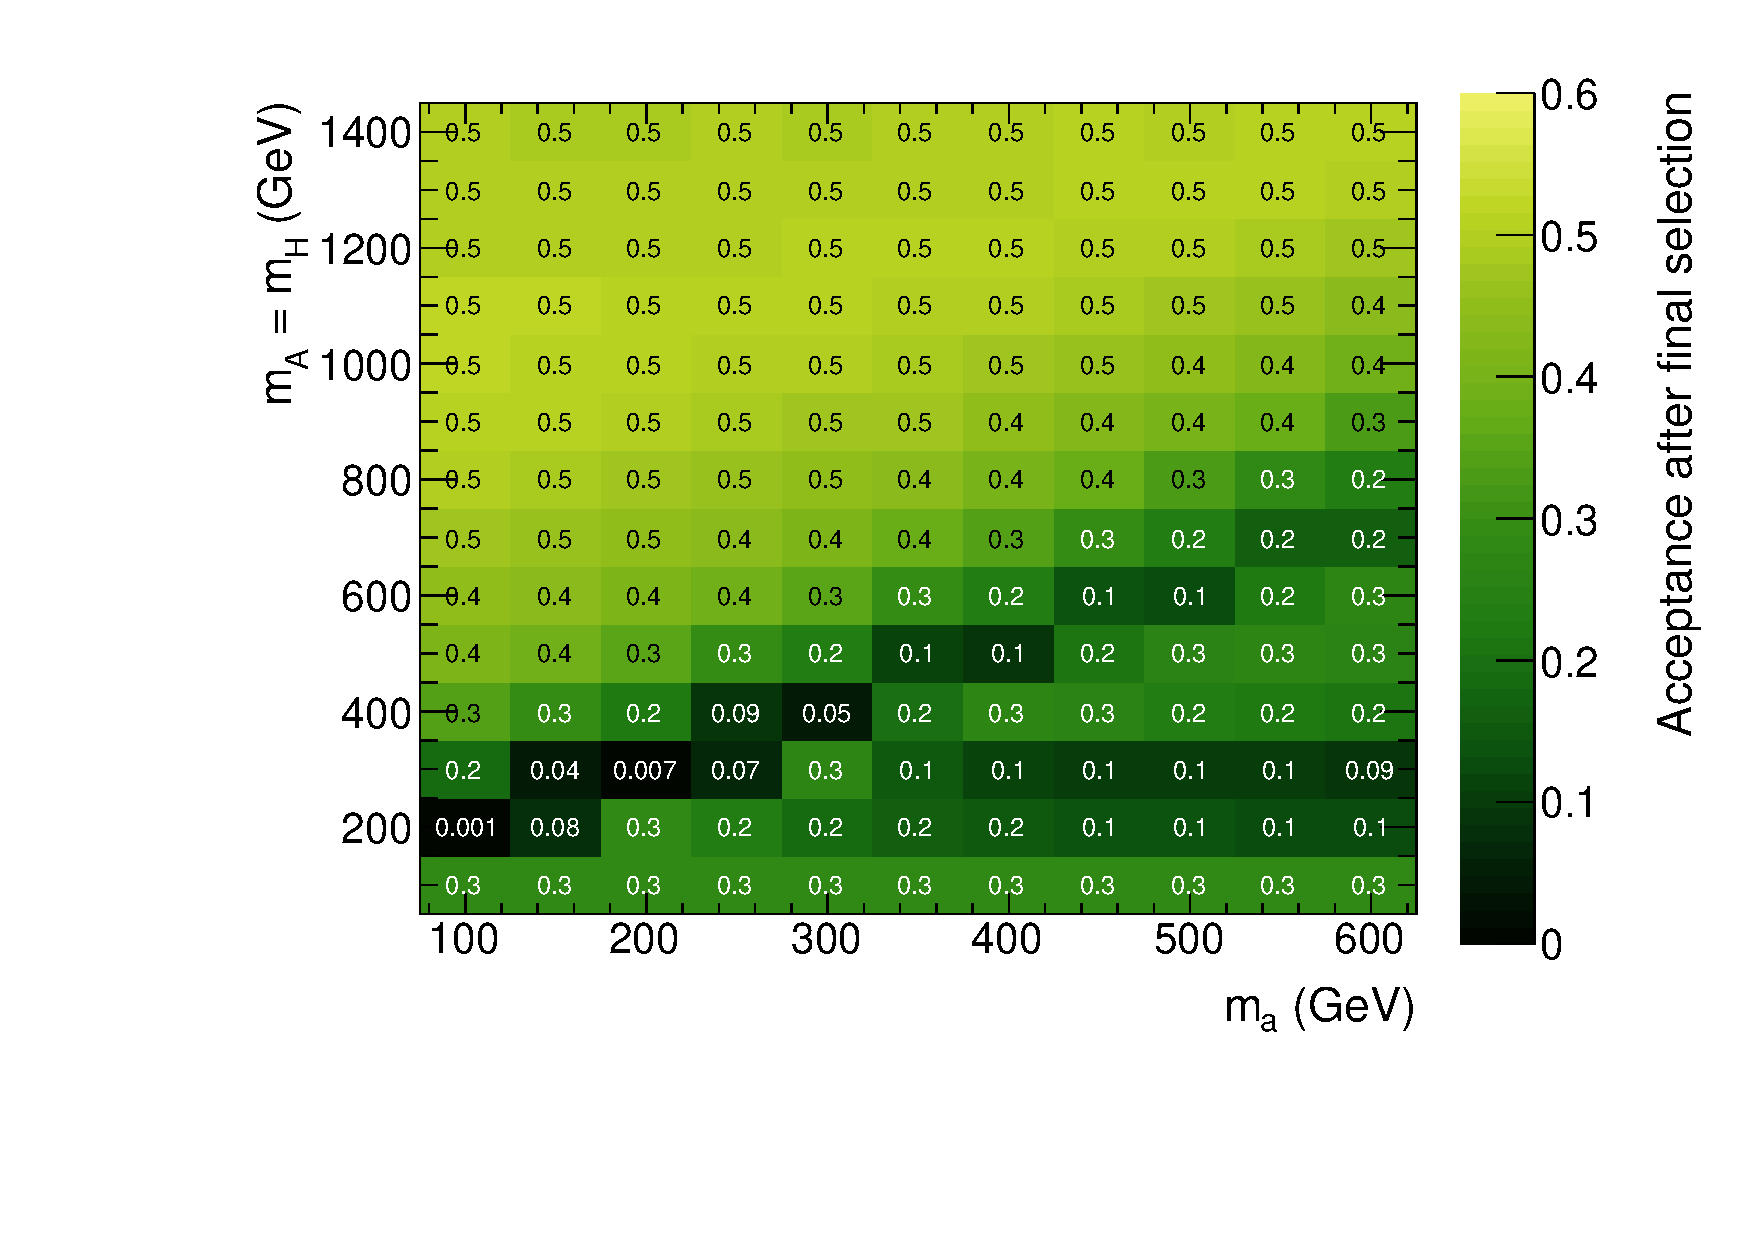
\includegraphics[width=\textwidth]{texinputs/04_grid/figures/monoz/leptonic/acceptance_dmwg-final_26300.pdf}
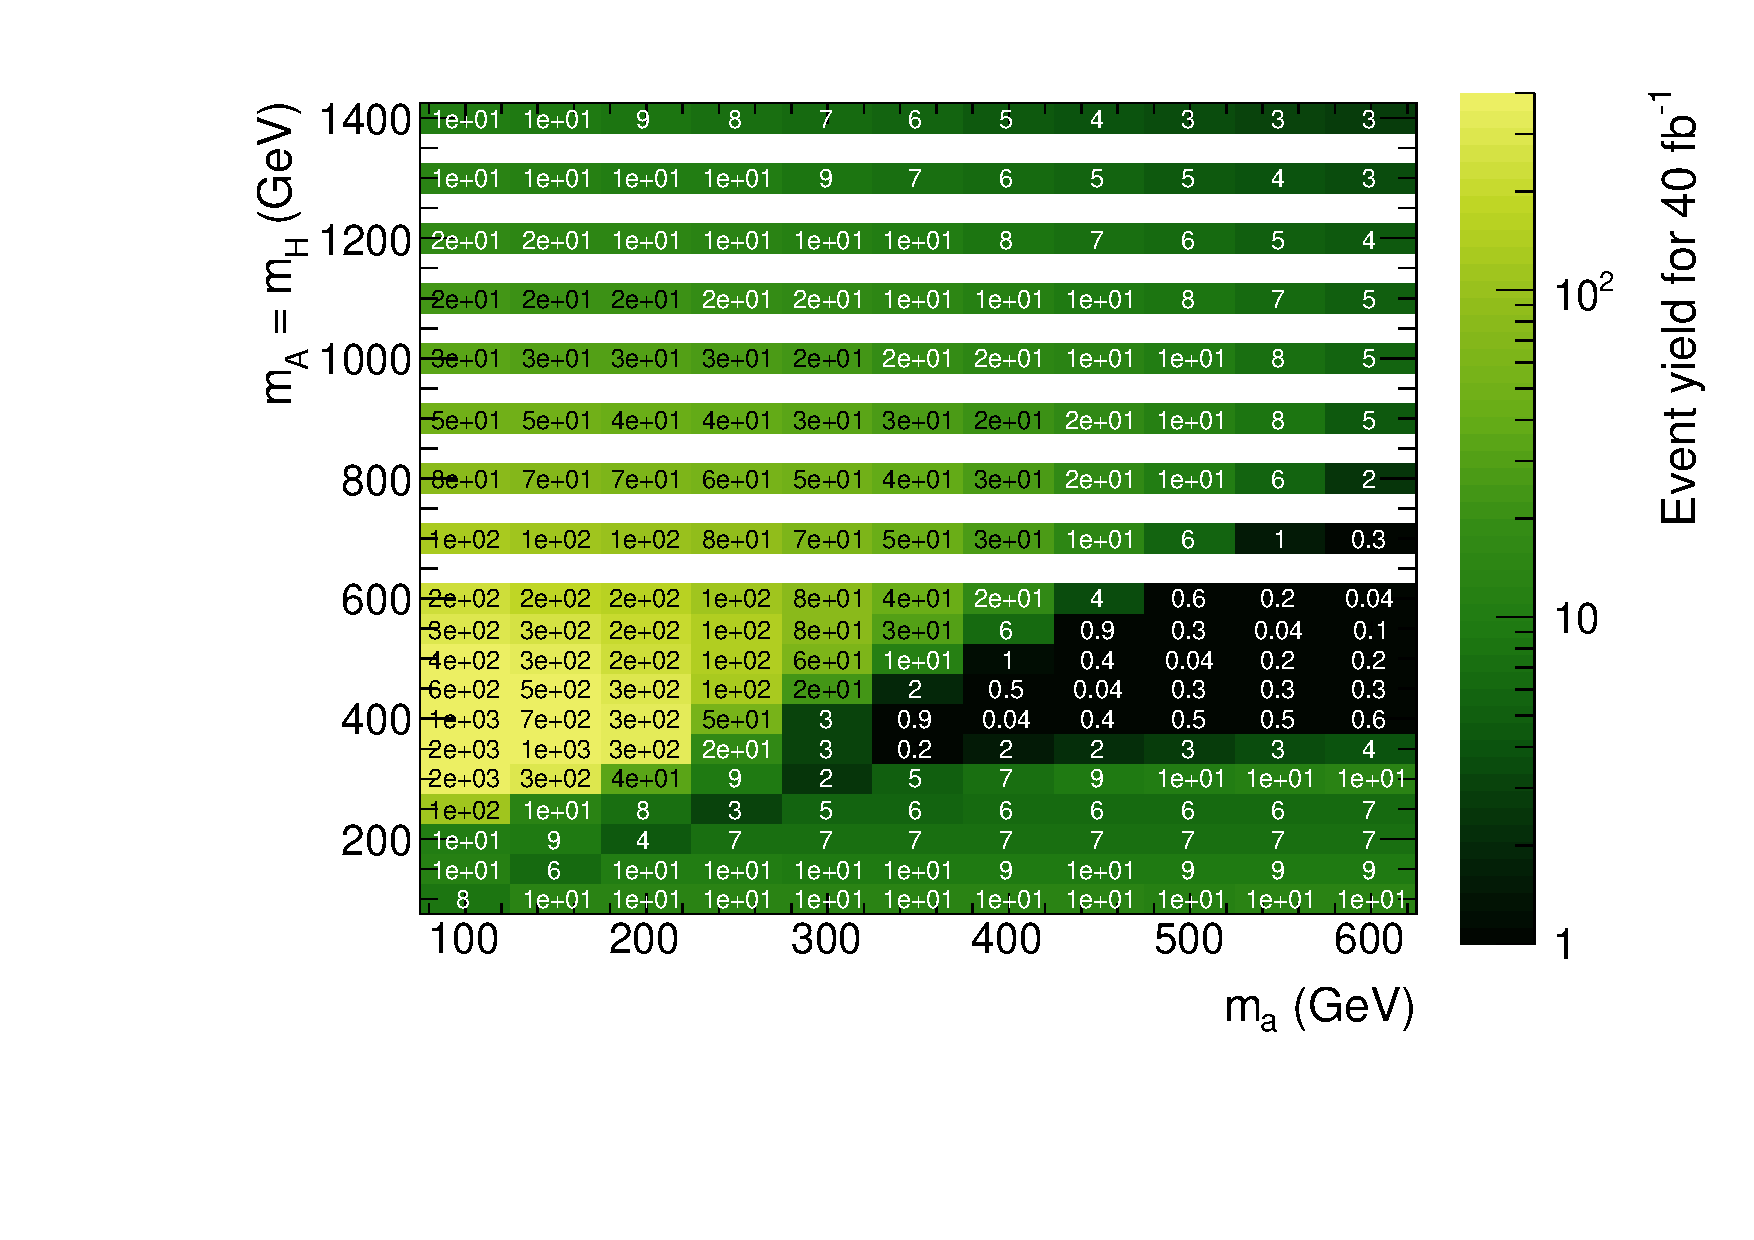
\includegraphics[width=\textwidth]{texinputs/04_grid/figures/monoz/leptonic/xs_2d_dmwg-final_26300_yield40fb.pdf}
\caption{Acceptance and event yields in the  \ma-\mA plane after applying the final selection. Event yields assume an integrated luminosity of $40~\ifb$. The acceptance is maximal for $\mA > \ma$, where it reaches 50 \%. In the inverted mass region $\mA < \ma$, lower values of 10-30\% are observed. In the intermediate region around $\mA \approx \ma + \mZ$, the acceptance is strongly suppressed as the a and Z bosons are produced approximately at rest.}
\label{fig:monoz_ll_acceptance}
\end{figure}

\begin{figure}
\centering
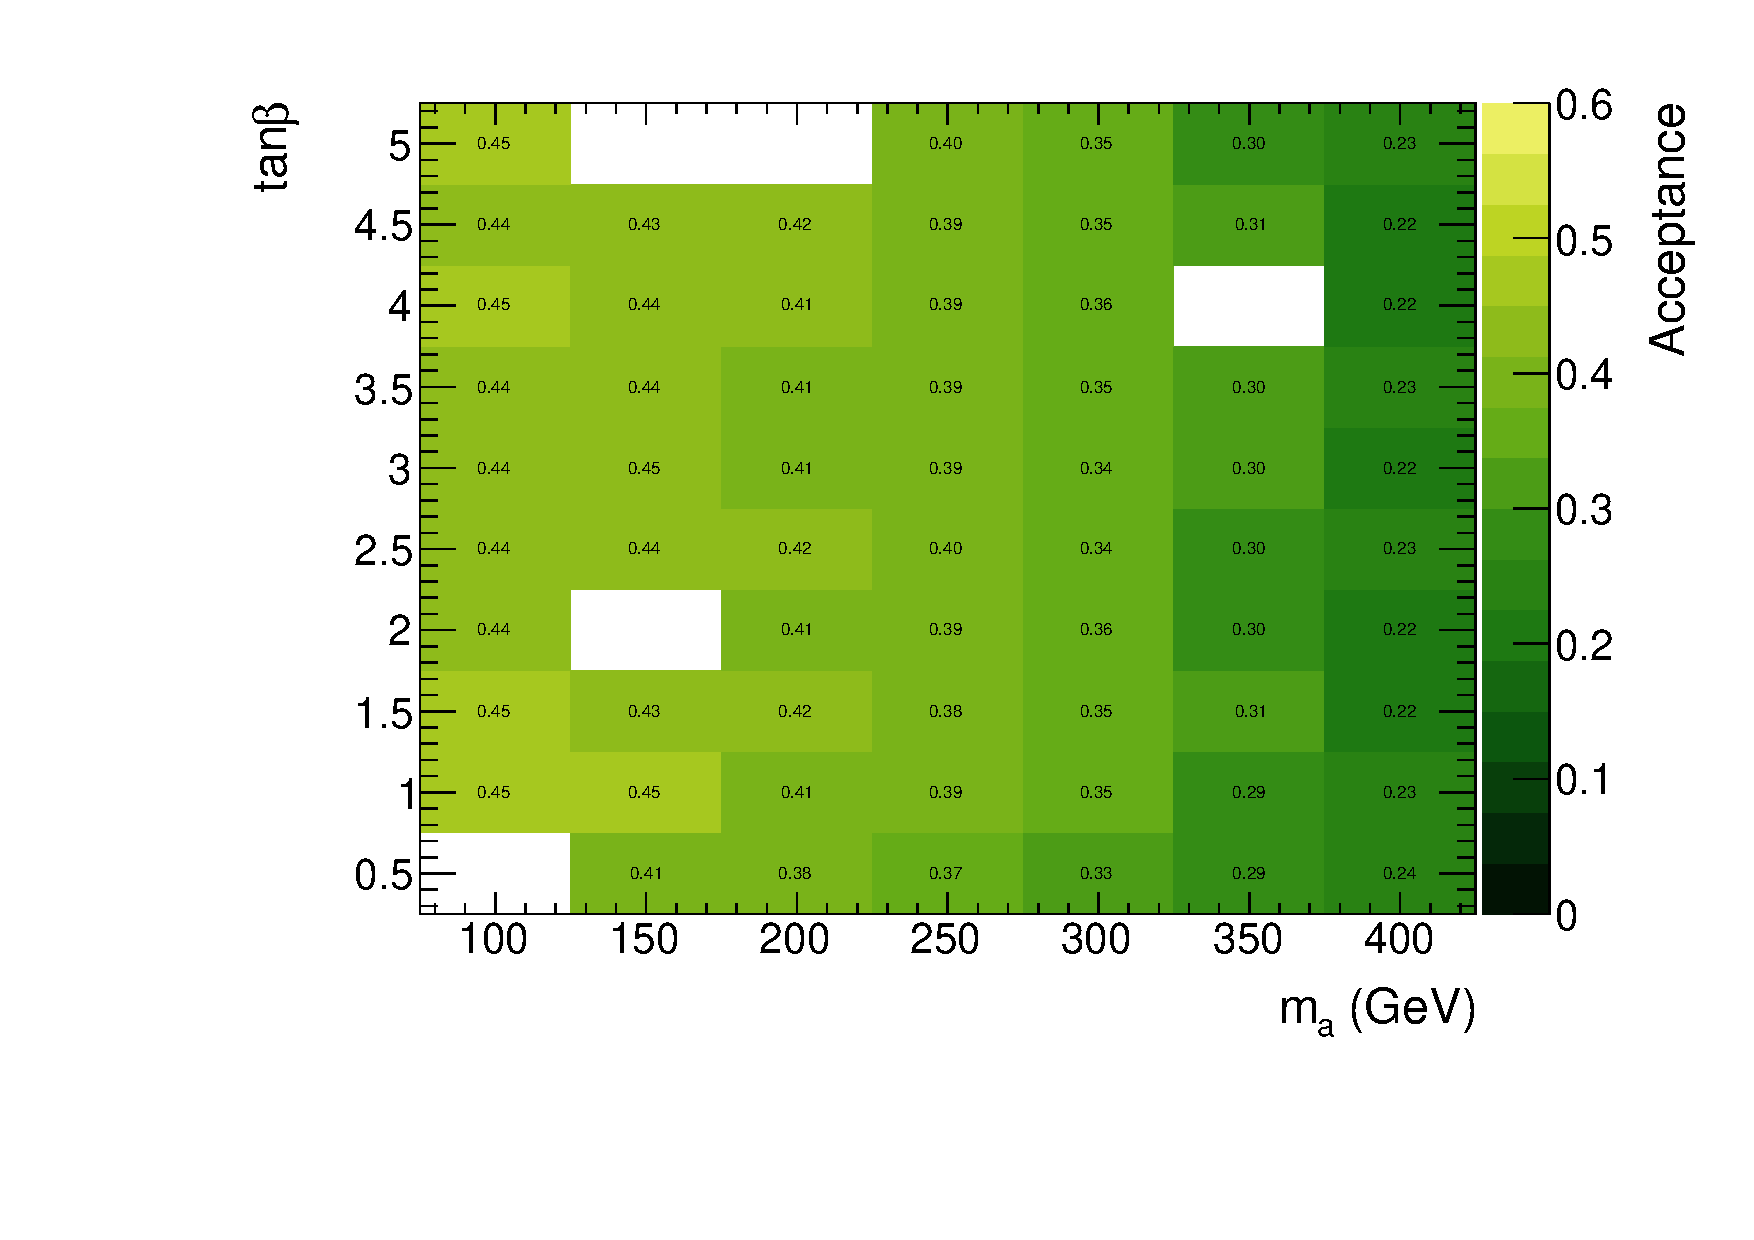
\includegraphics[width=0.9\textwidth]{texinputs/04_grid/figures/monoz/leptonic/tanbma_ae_ll.pdf}
\caption{Acceptances across the \ma-\tanb scan.  Acceptance is flat over \tanb for constant values of \ma.}
\label{fig:monoz_ll_tanbma_acceptance}
\end{figure}

\begin{figure}
\centering
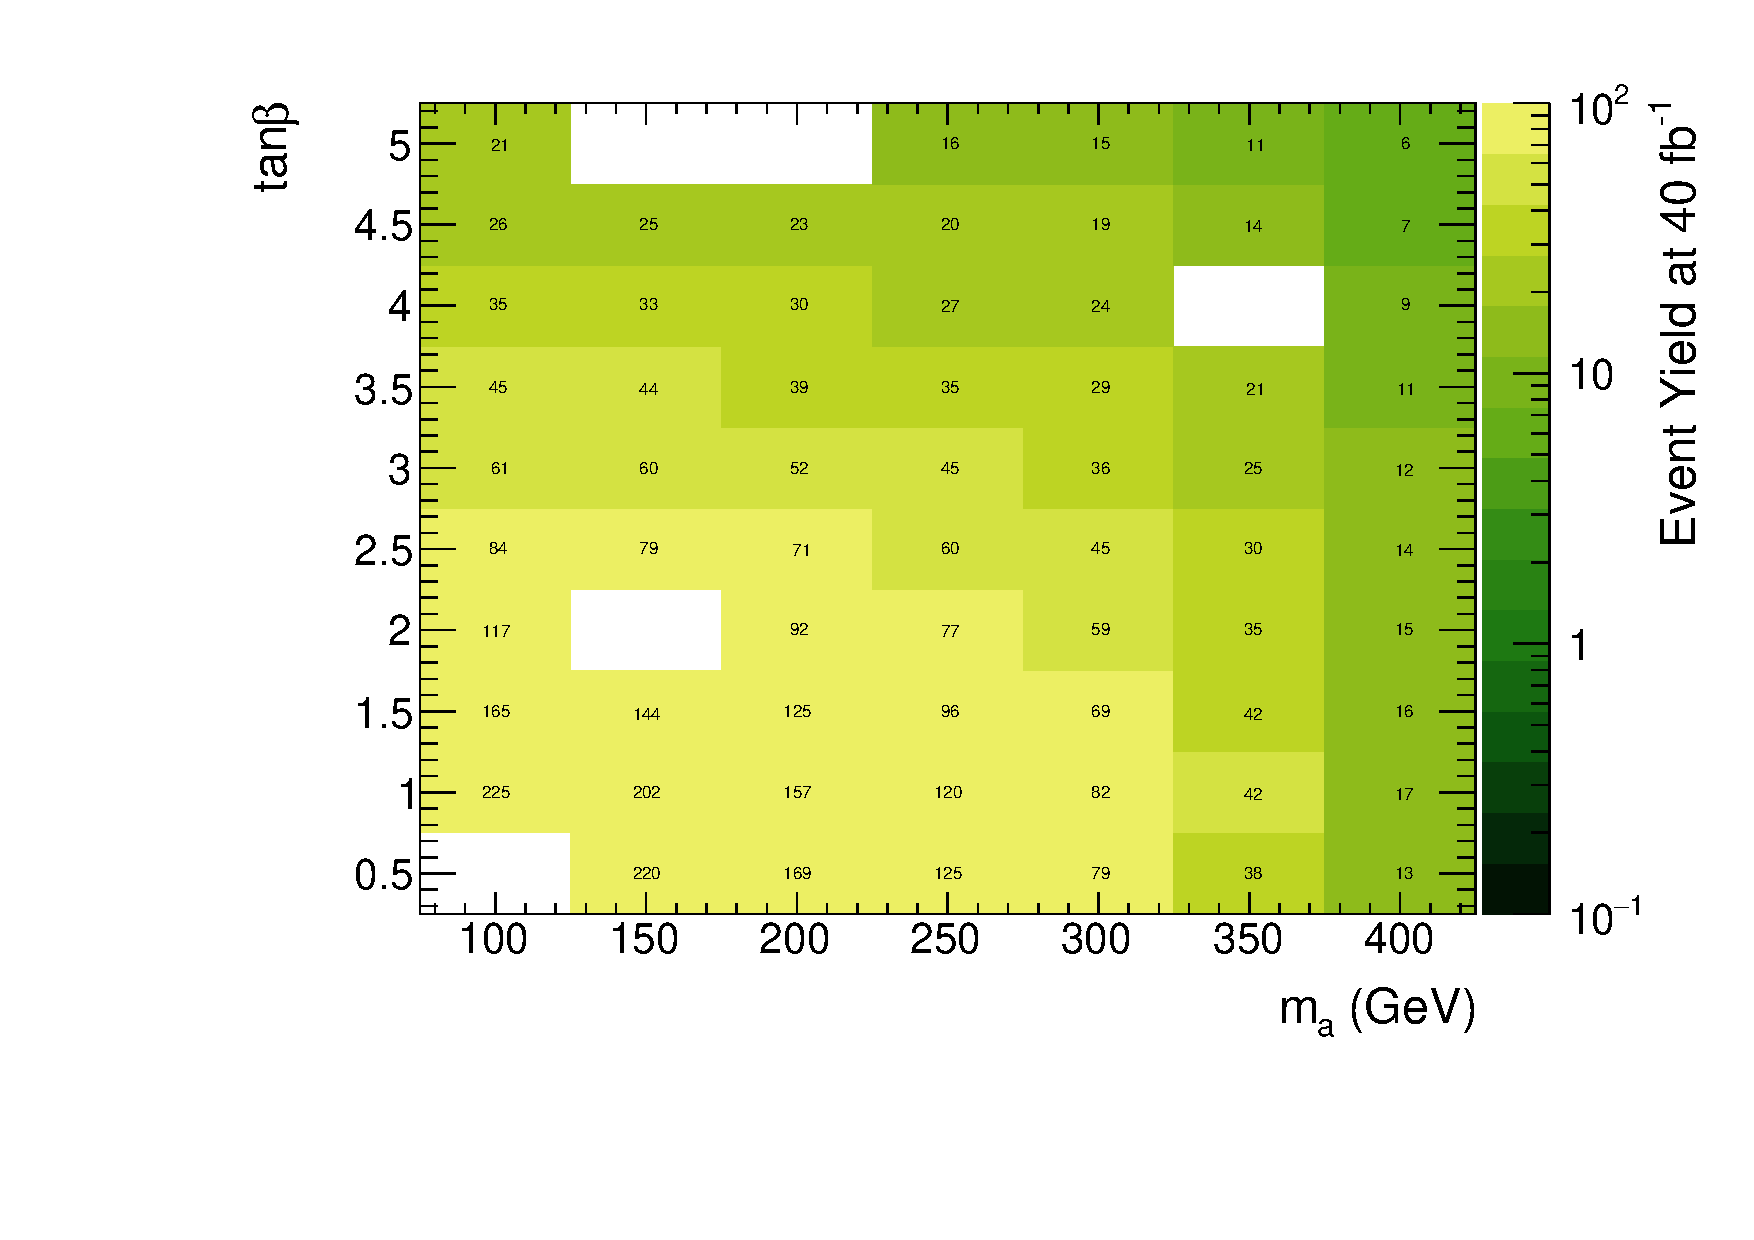
\includegraphics[width=0.9\textwidth]{texinputs/04_grid/figures/monoz/leptonic/tanbma_yield_ll.pdf}
\caption{Event yield in the \ma-tanBeta grid, for an integrated luminosity of $40~\ifb$.  The number of expected events diminshes with increasing tanBeta and \ma.  \mA fixed to 600 GeV and sinTheta to 0.35}
\end{figure}



\begin{figure}
%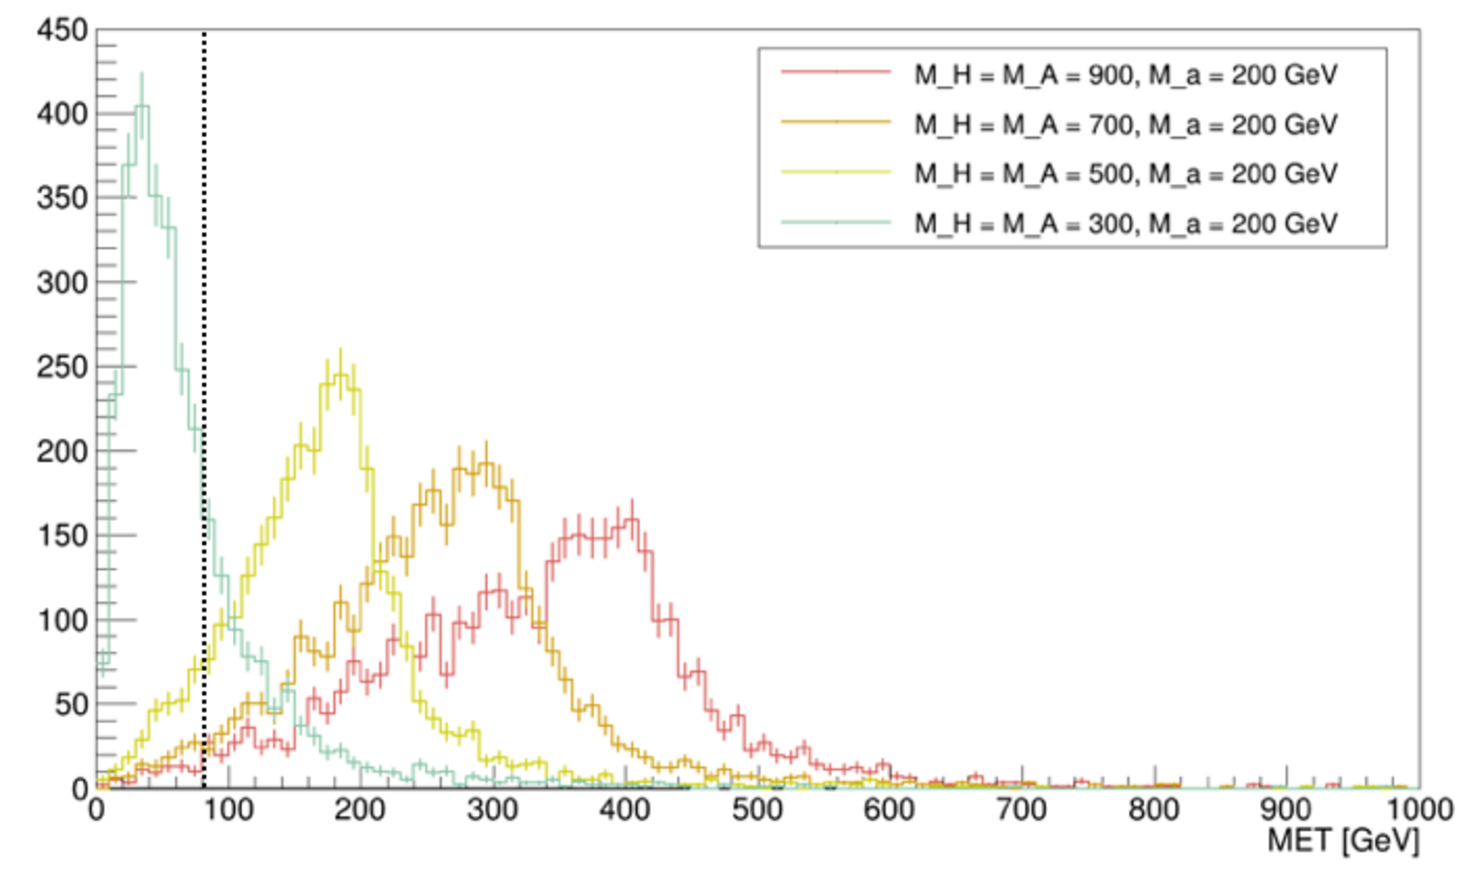
\includegraphics[width=0.9\textwidth]{texinputs/04_grid/figures/monoz/leptonic/mA_Scan.pdf}
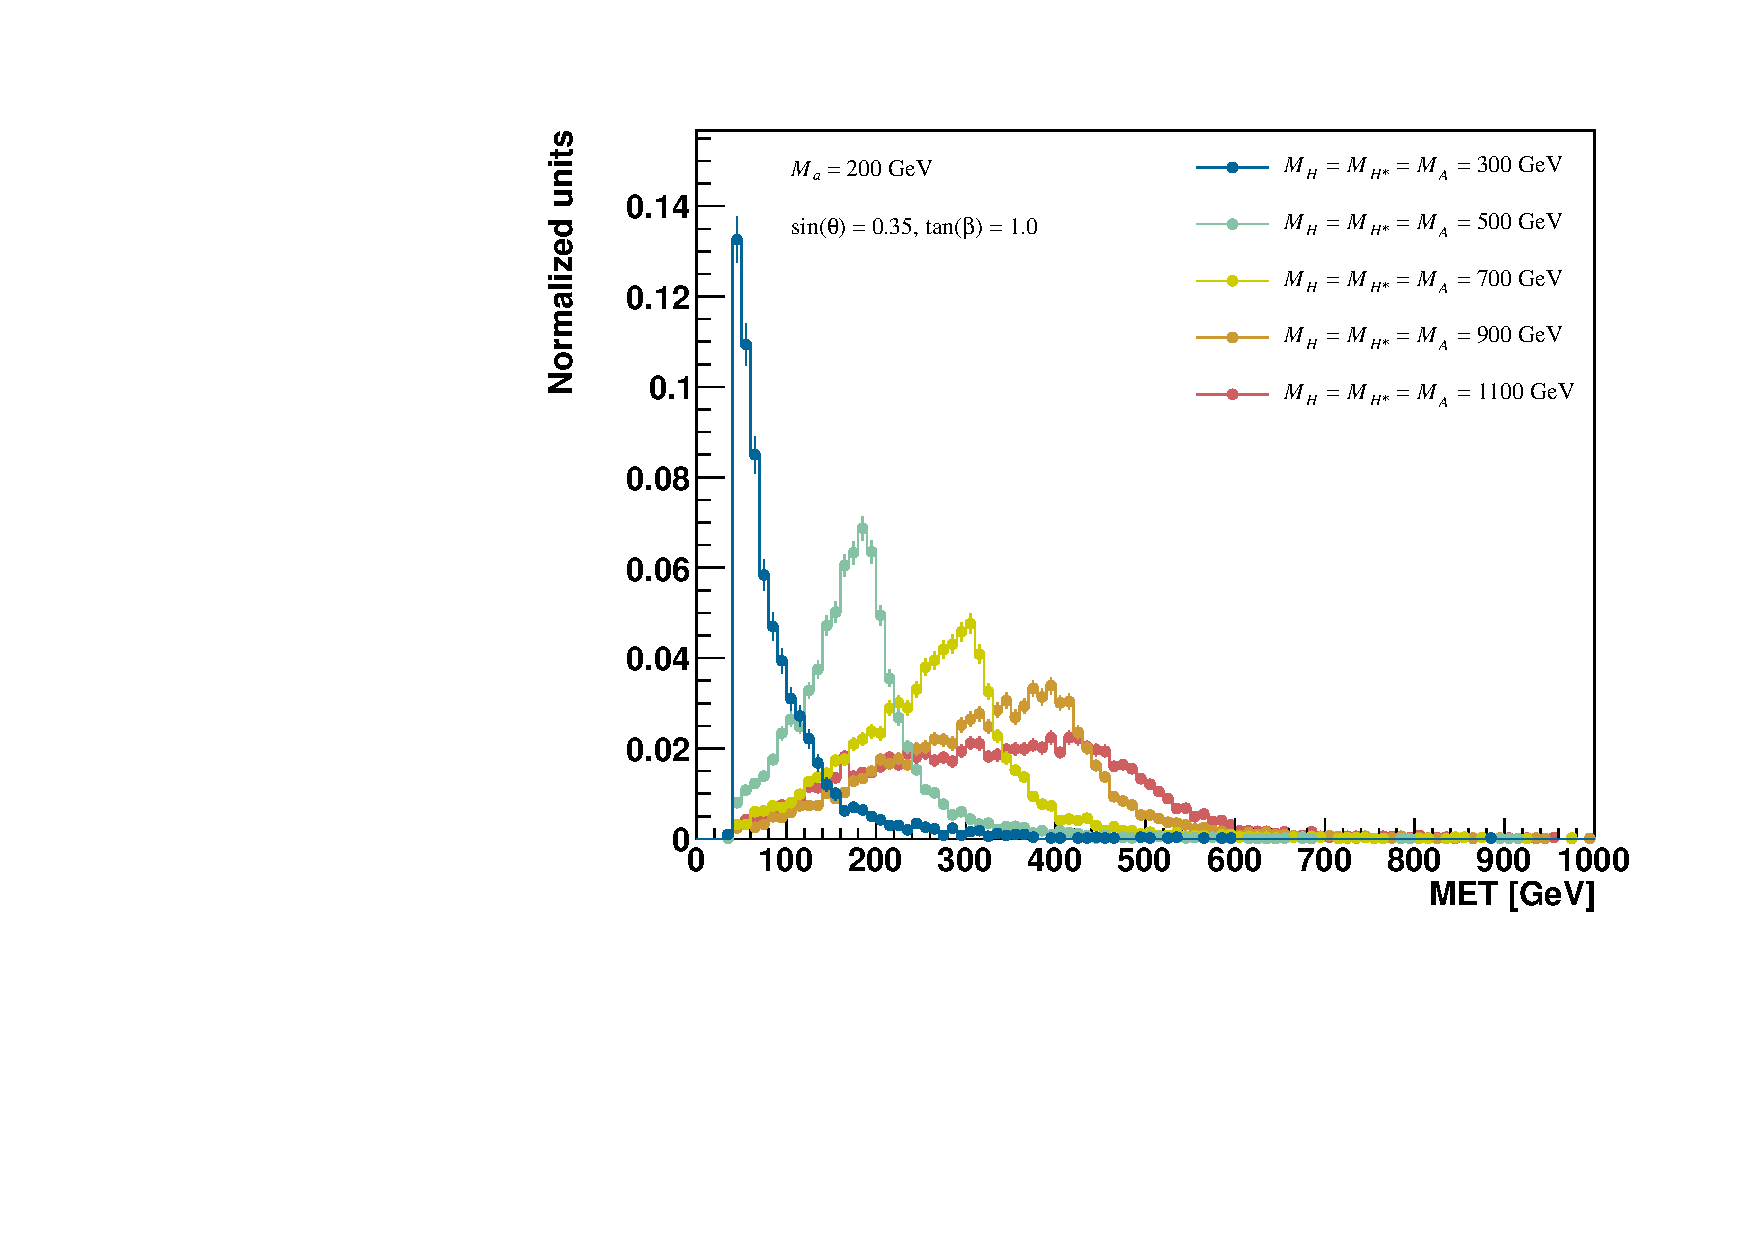
\includegraphics[width=0.9\textwidth]{texinputs/04_grid/figures/monoz/leptonic/mAscan_for_ma200.pdf}
\caption{The position of the Jacobian peak in the \MET distribution depends on the values of \mH, \ma, and $M_{Z}$.  This figure shows a scan of \mH values for fixed \ma and \mA = \mH.  Increasing the difference between \mH and \ma shifts the location of the peak towards high energies, whereas for small mass splittings the \MET distribution is soft and most events will fail to pass the \MET selection criteria.}   
\label{fig:monoz_ll_mA_scan}
\end{figure}

\begin{figure}
\centering
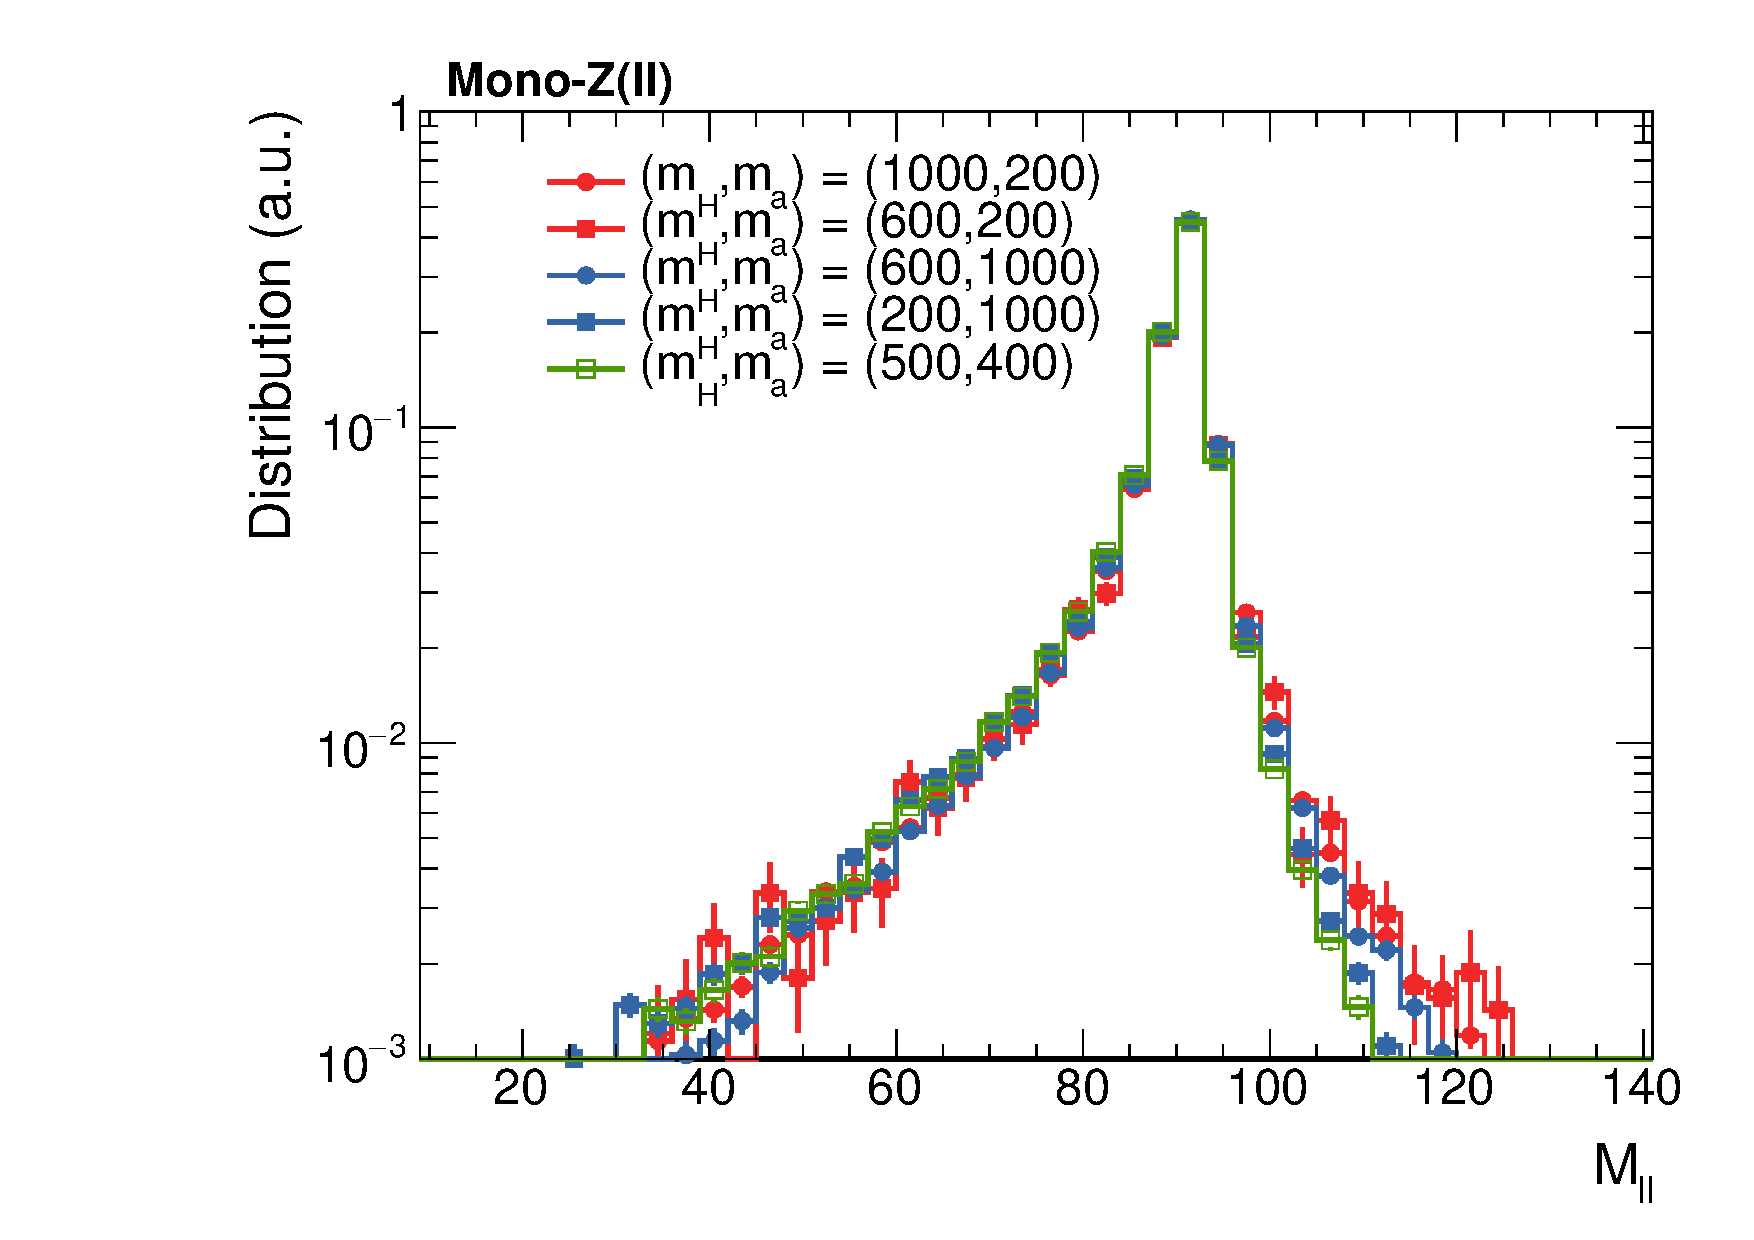
\includegraphics[width=0.45\textwidth]{texinputs/04_grid/figures/monoz/leptonic/inclusive_h_mz_lep.pdf}
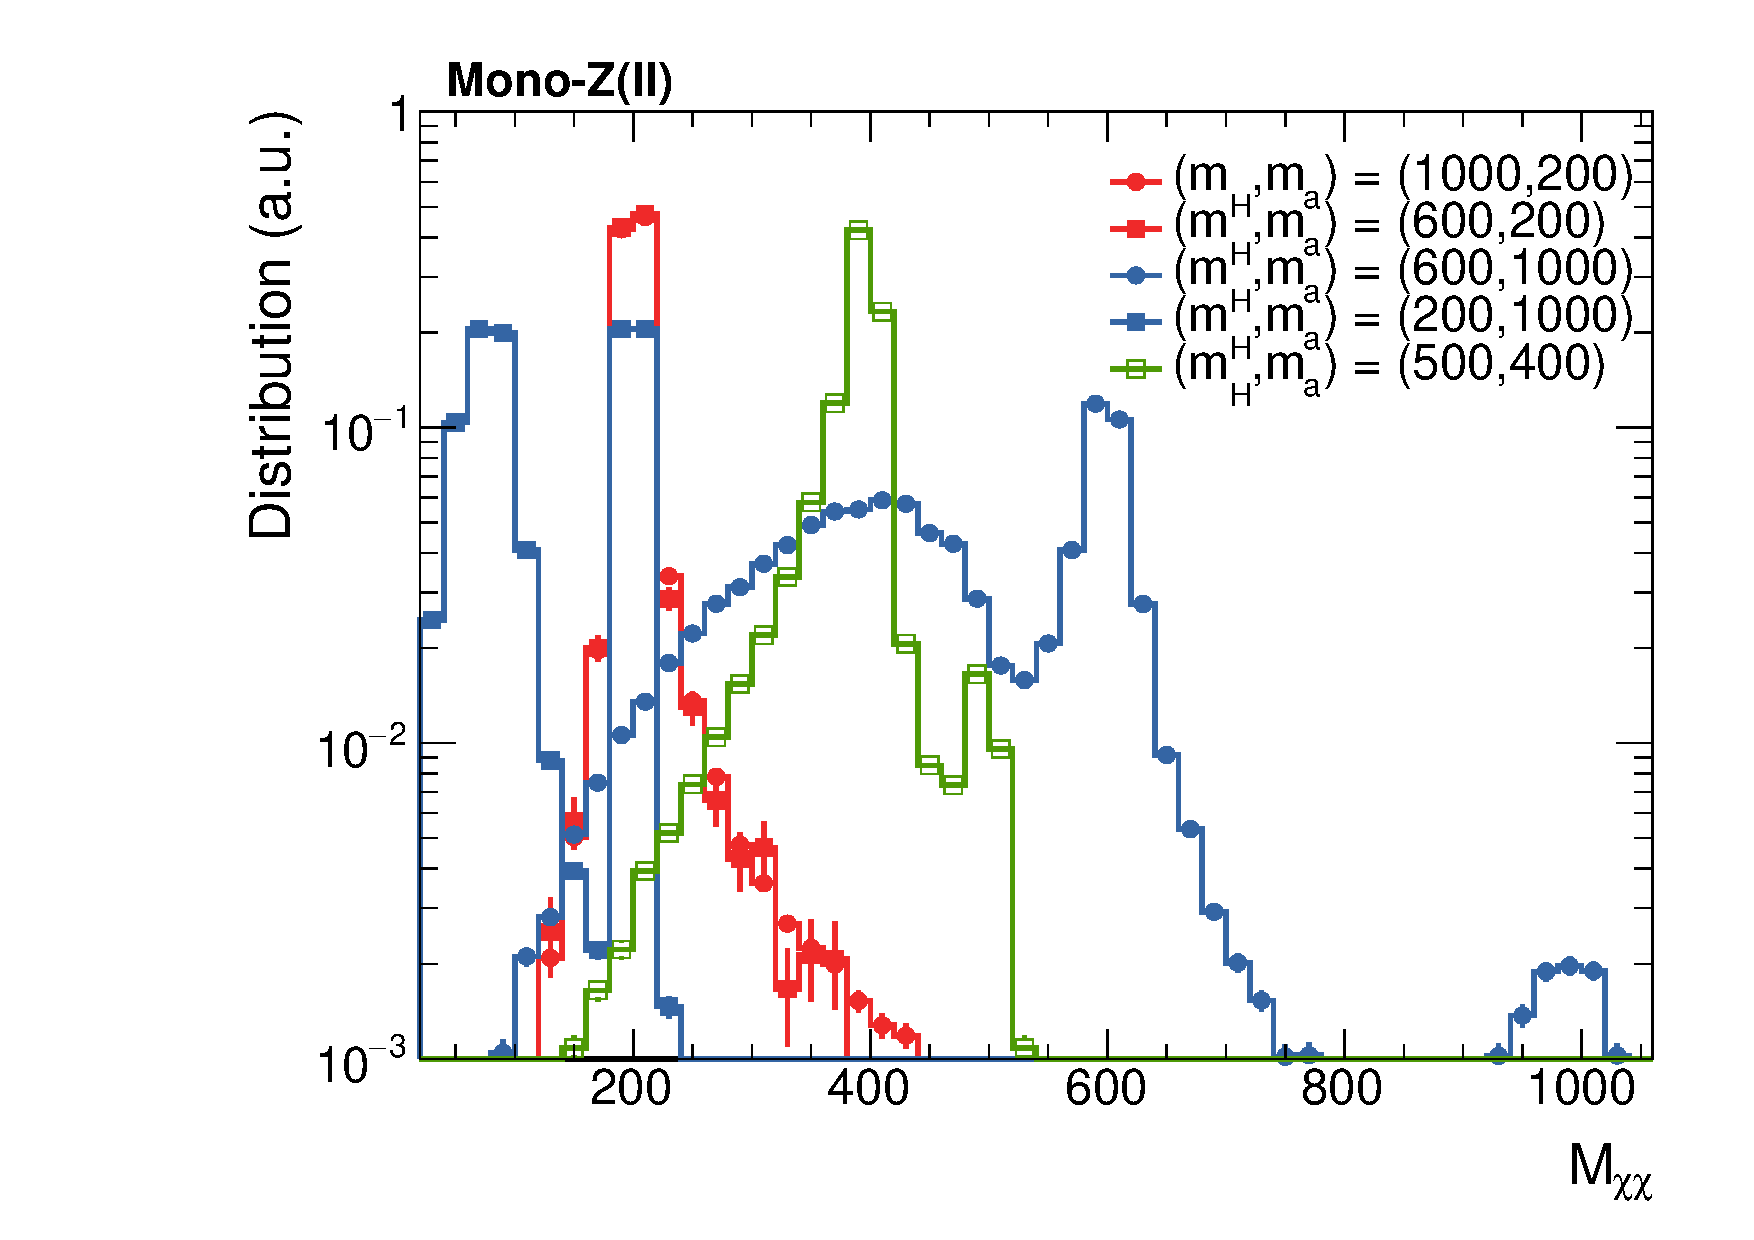
\includegraphics[width=0.45\textwidth]{texinputs/04_grid/figures/monoz/leptonic/inclusive_h_m_med_dm.pdf}
\caption{Distributions of the invariant mass of the dilepton (left) and $\chi\overline{\chi}$ systems (right) with no selection applied in addition to the generation cuts. The $M_{ll}$ distribution is centered around the Z boson mass independent of the chosen parameter point, indicating that there is no contribtion from $\gamma*$ exchange. The $M_{\chi\overline{\chi}}$ distribution }
\label{fig:monoz_kin_inclusive}
\end{figure}

\begin{figure}
\centering
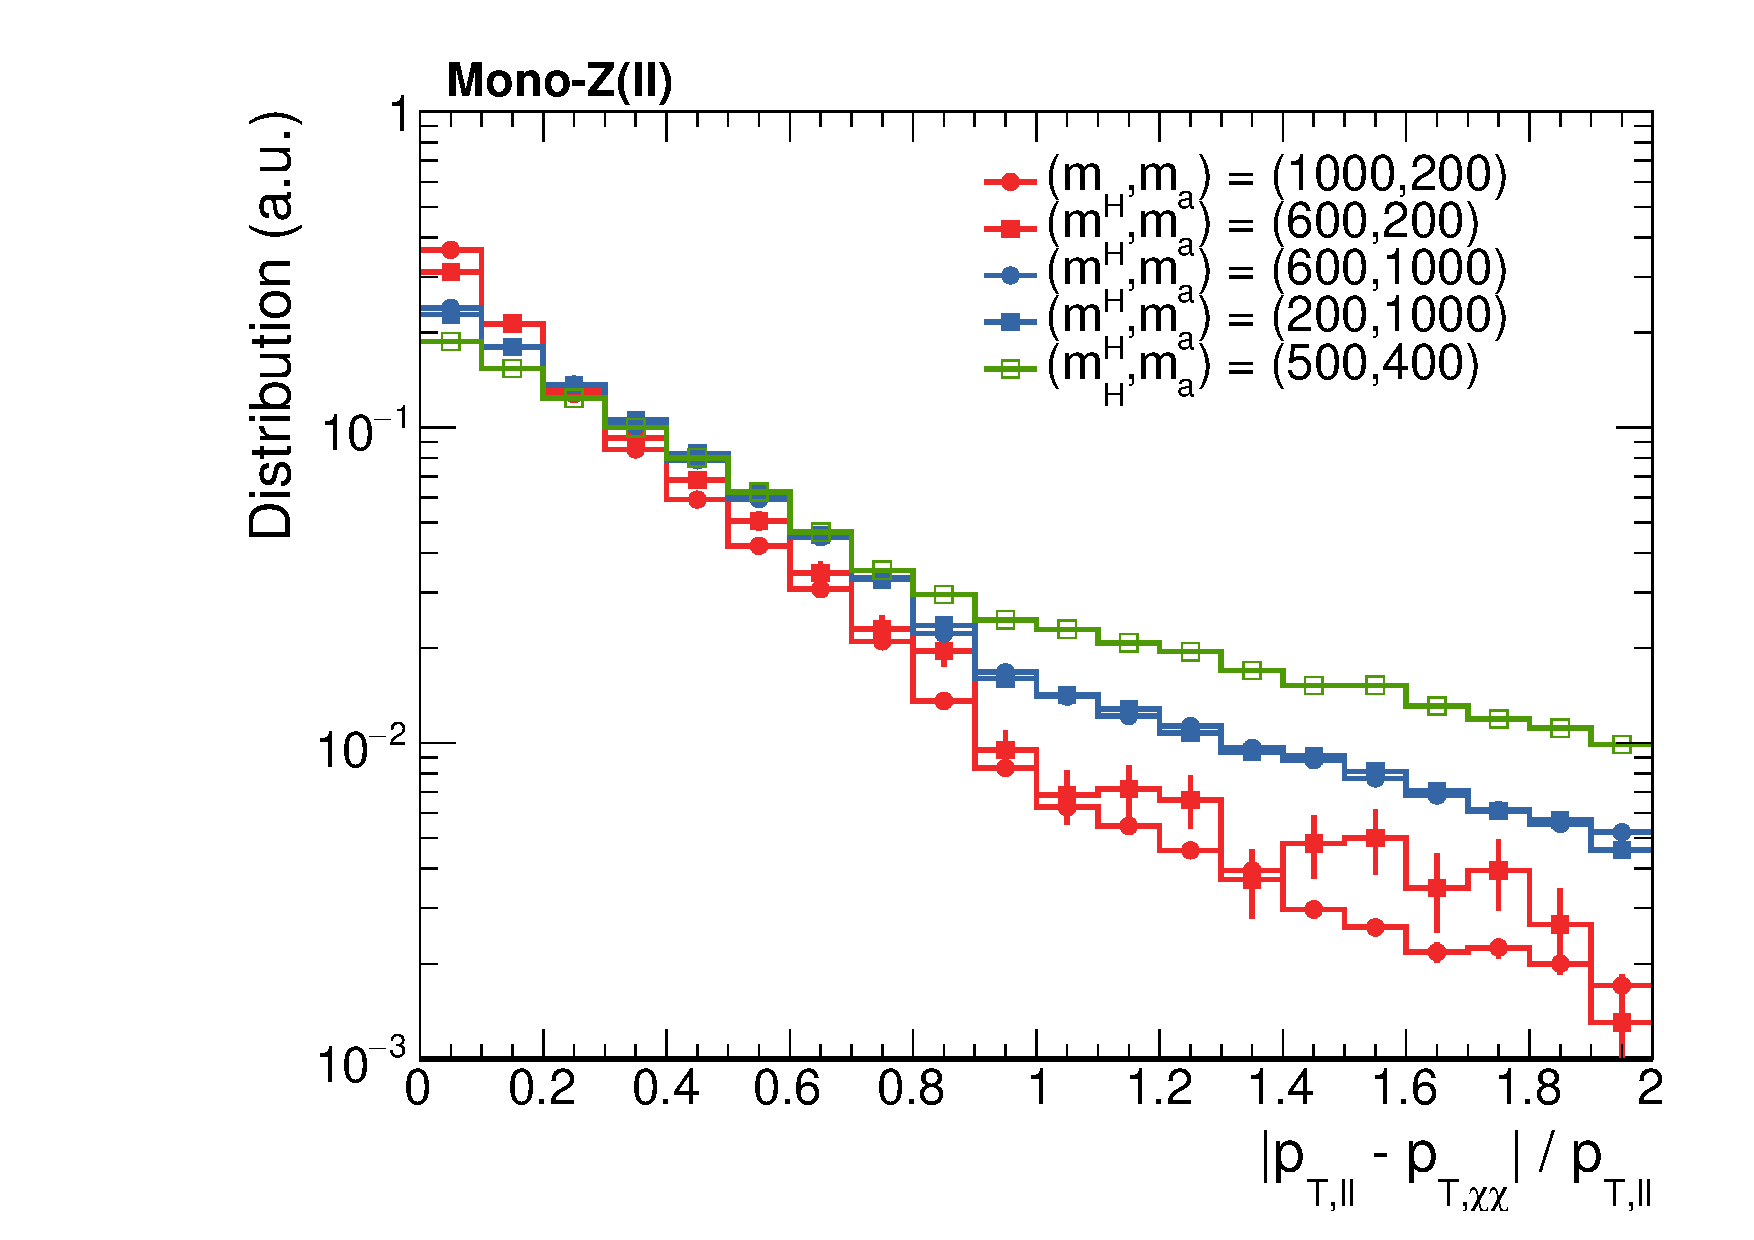
\includegraphics[width=0.45\textwidth]{texinputs/04_grid/figures/monoz/leptonic/presel_h_balance.pdf}
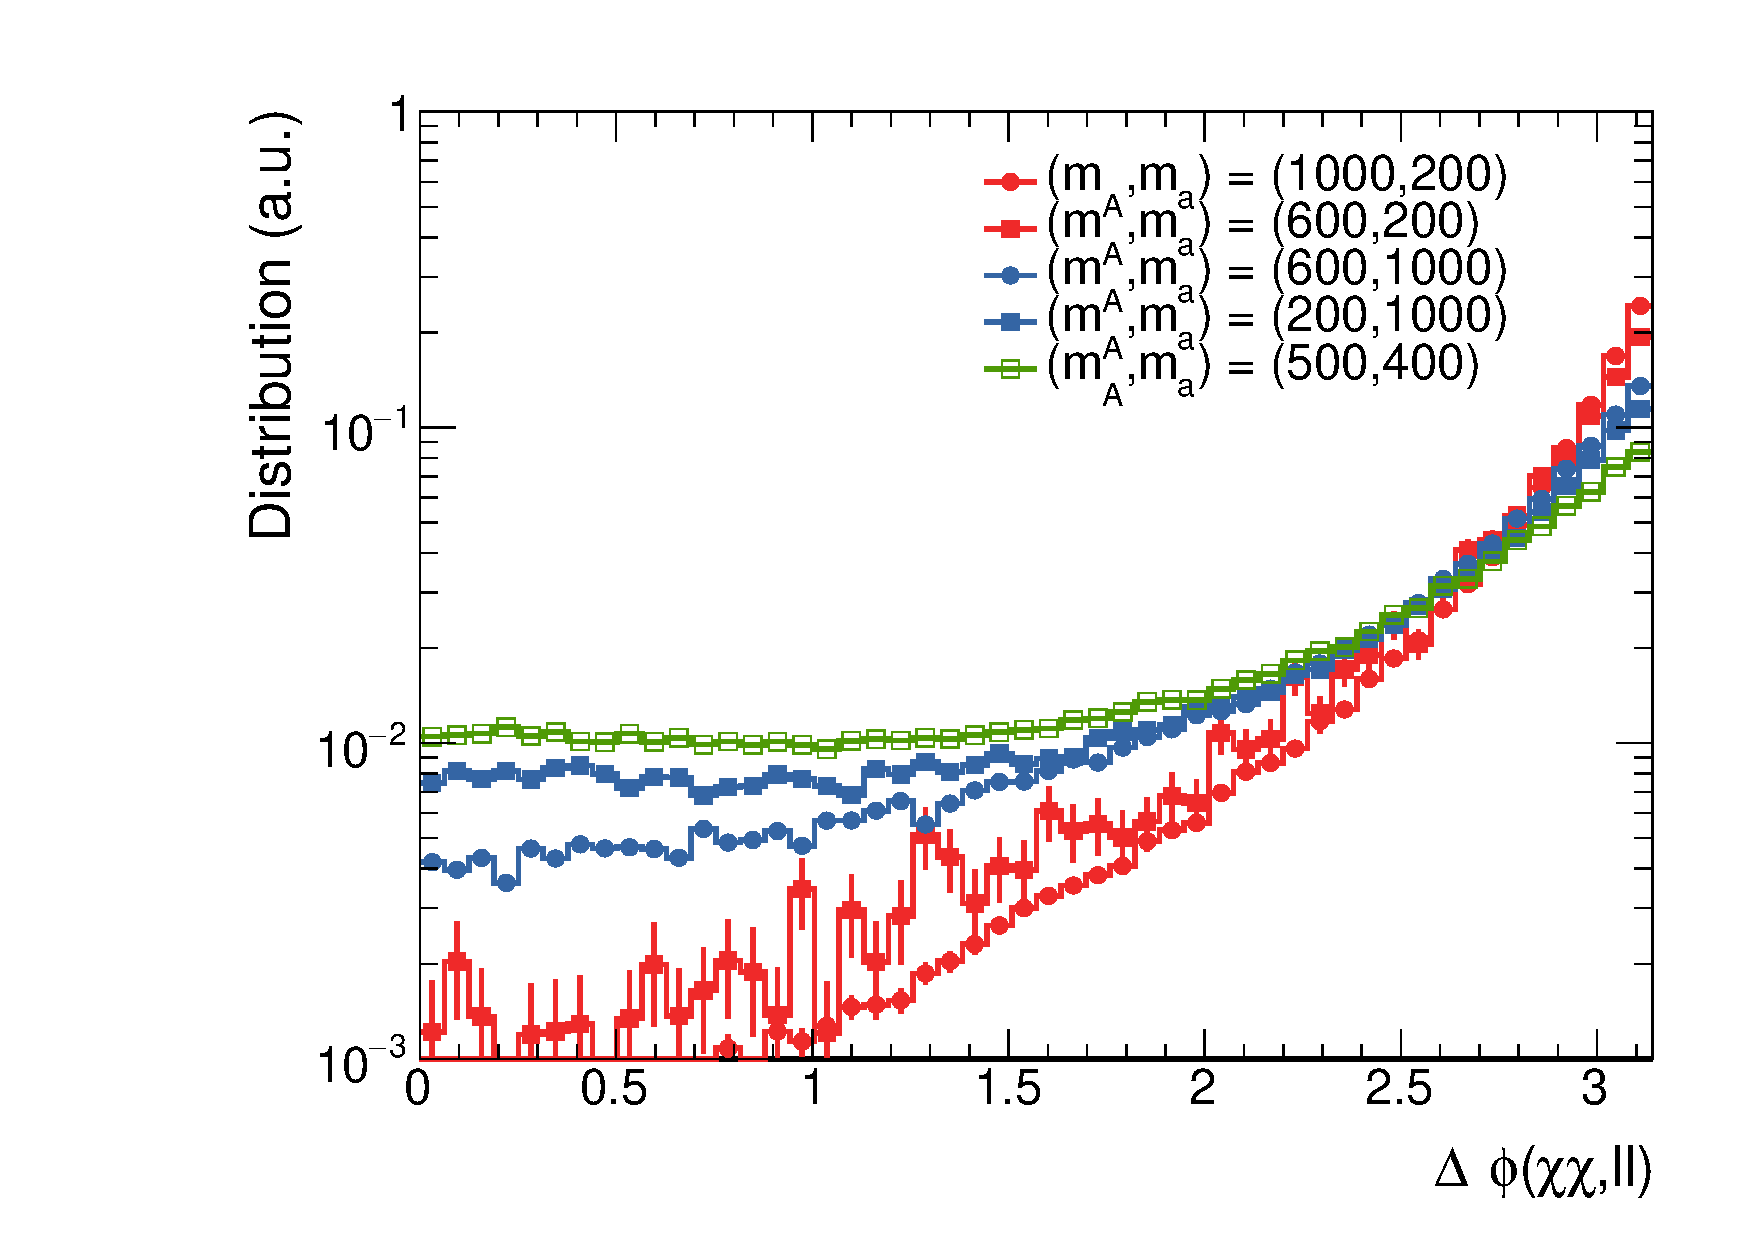
\includegraphics[width=0.45\textwidth]{texinputs/04_grid/figures/monoz/leptonic/presel_h_dphi_met_ll.pdf}
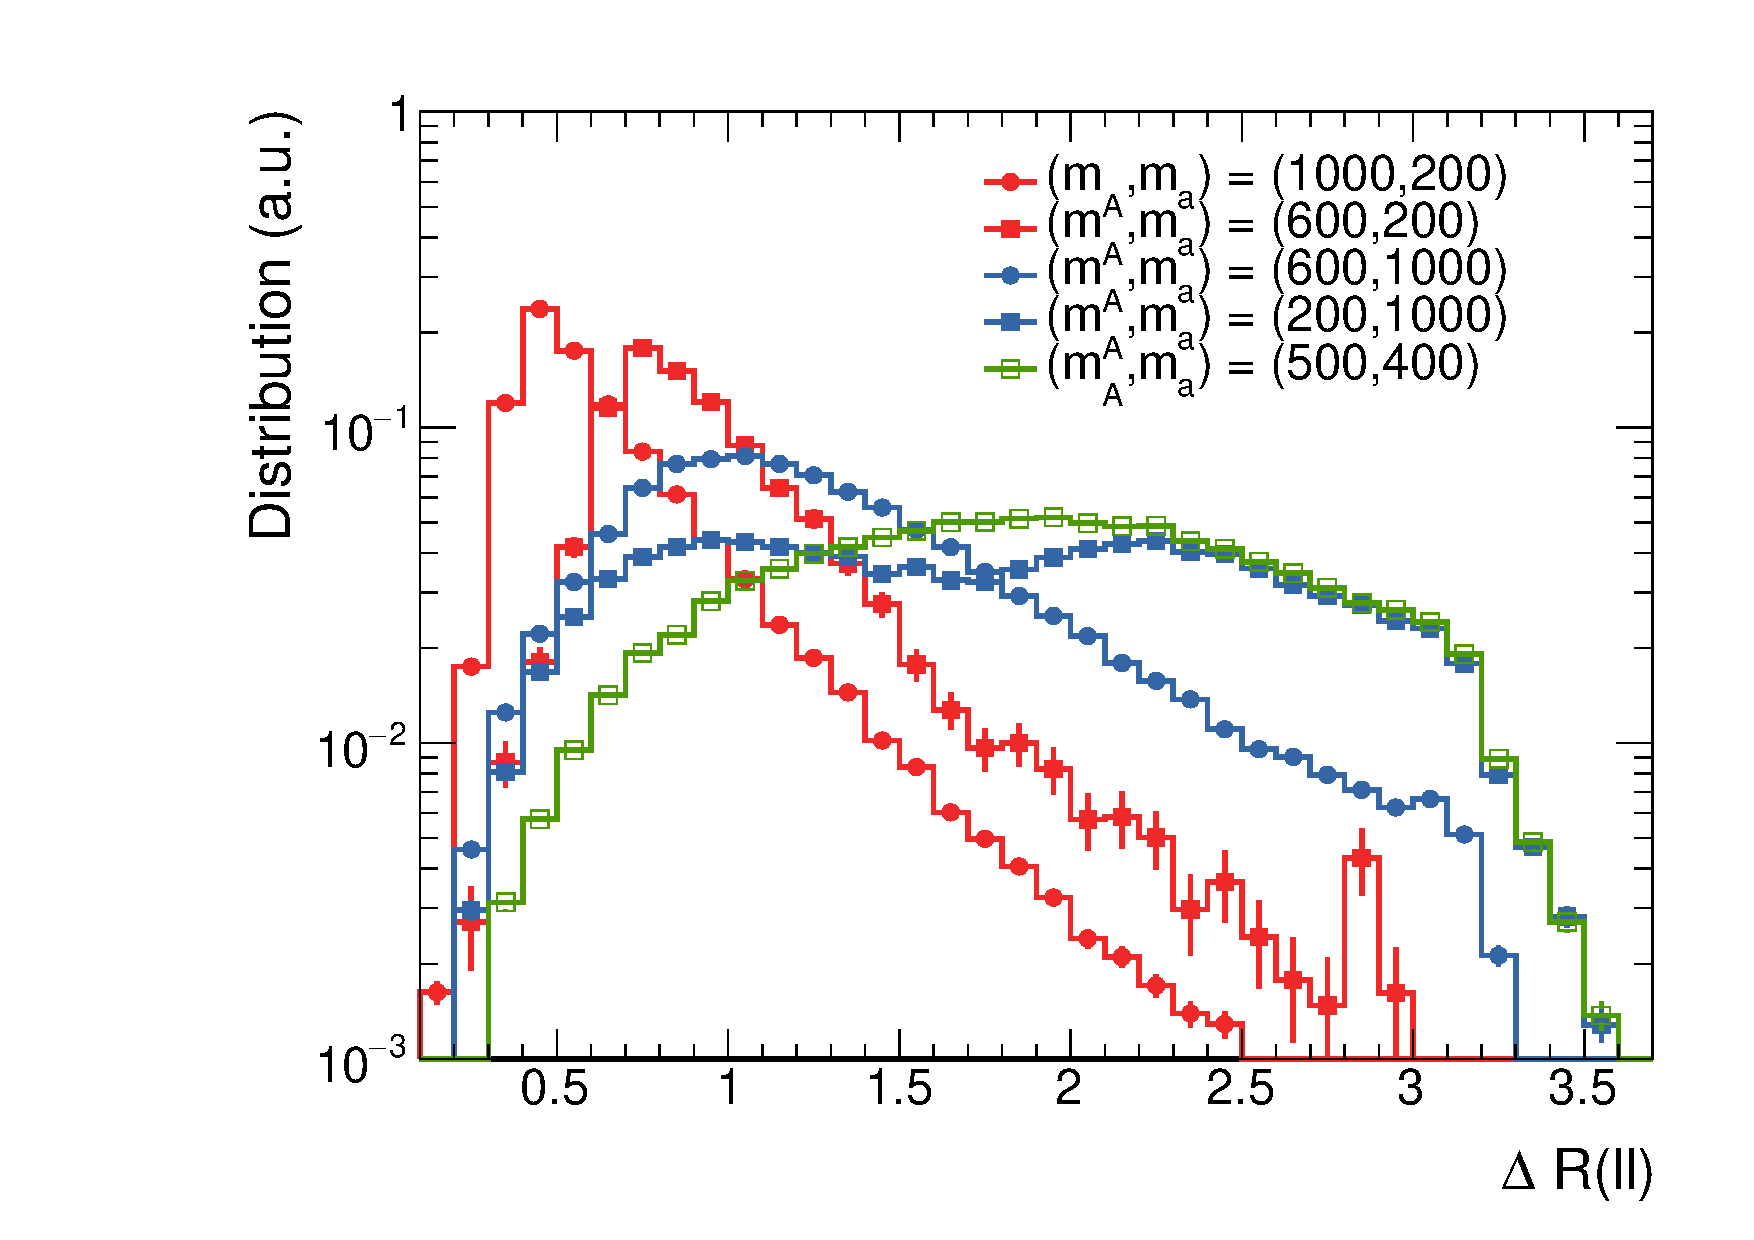
\includegraphics[width=0.45\textwidth]{texinputs/04_grid/figures/monoz/leptonic/presel_h_dr_ll.pdf}
\caption{Distributions of the main selection variables after preselection: \pt balance (top panel), $\Delta\Phi$ (middle) and $\Delta R$ (bottom). The shown parameter points illustrate the different qualitative behavior in the three different mass regions. }
\label{fig:monoz_kin_presel}
\end{figure}


\begin{figure}
\centering
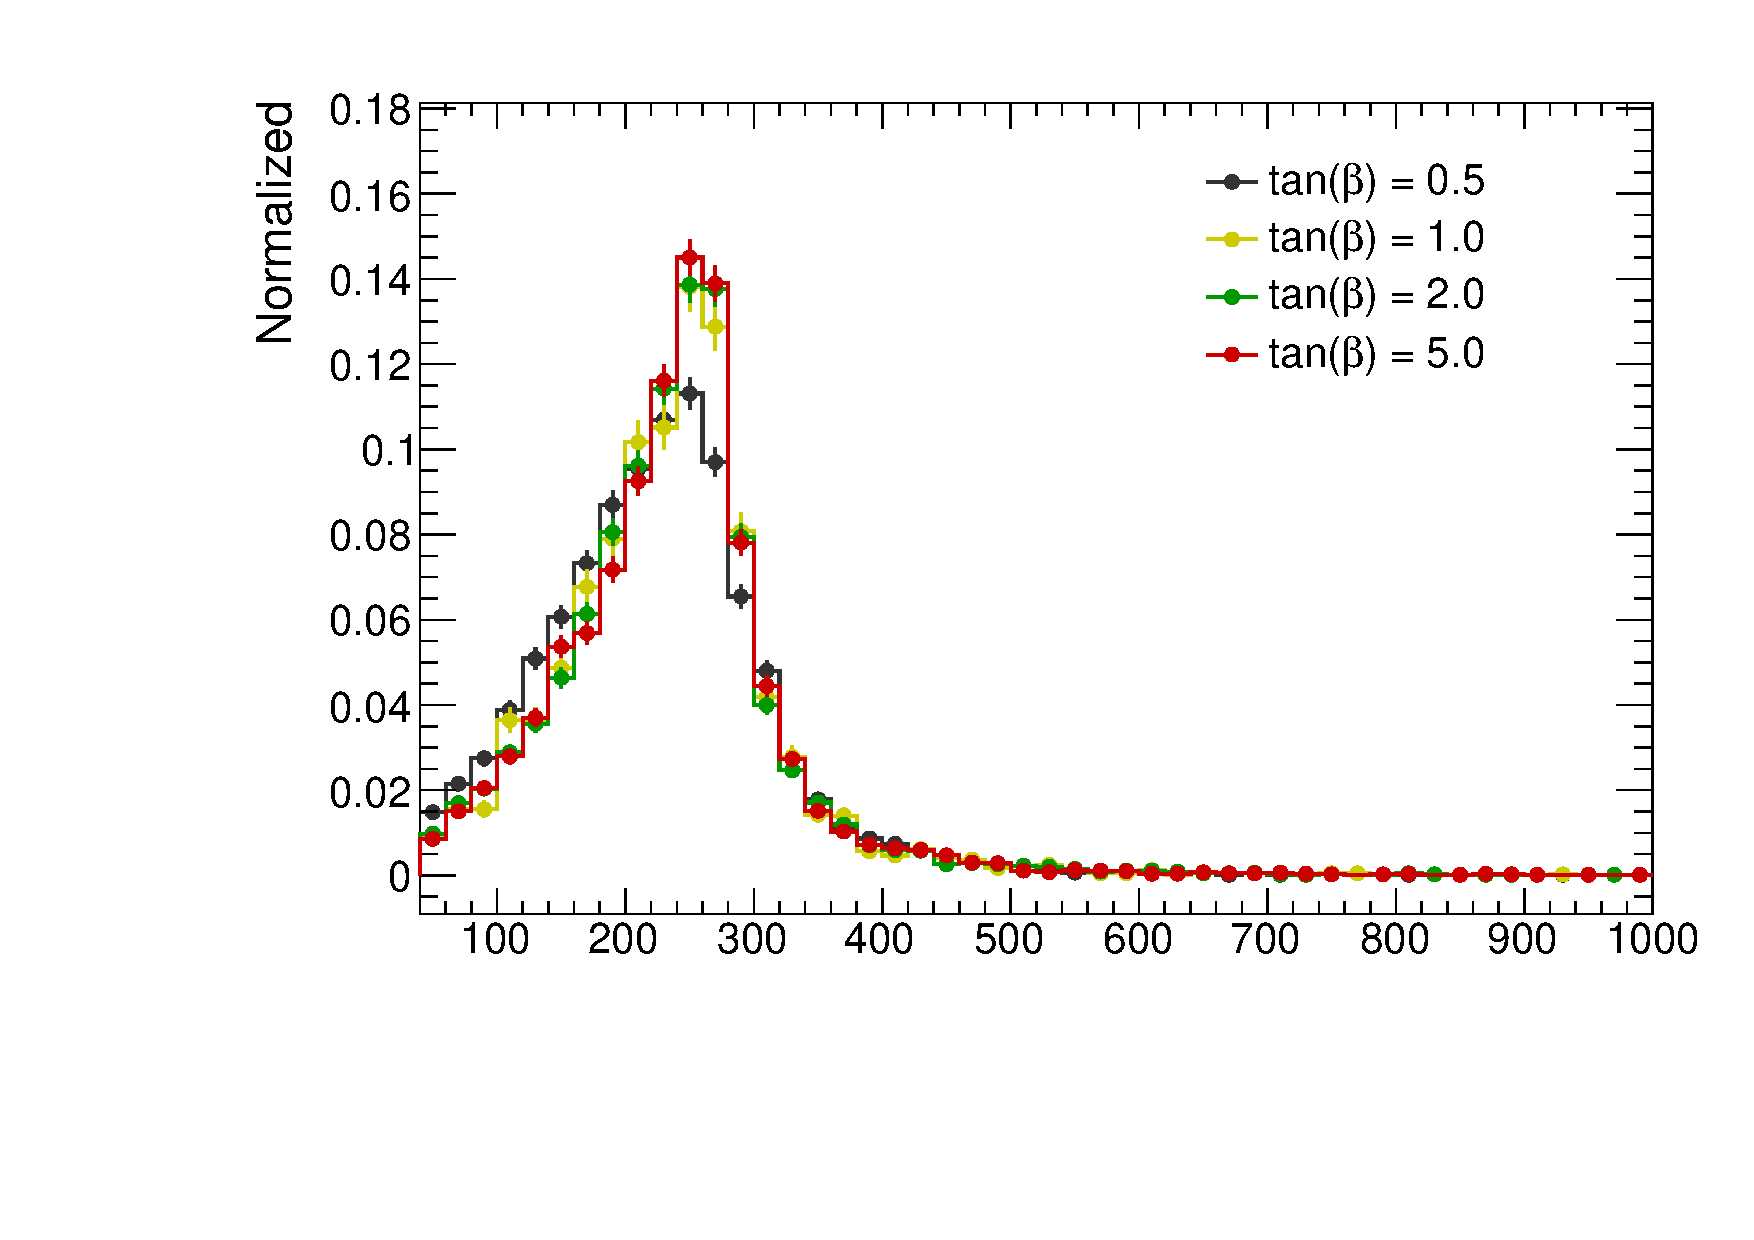
\includegraphics[width=0.48\textwidth]{texinputs/04_grid/figures/monoz/leptonic/TanbScan_mA600_ma150_MET.pdf} 
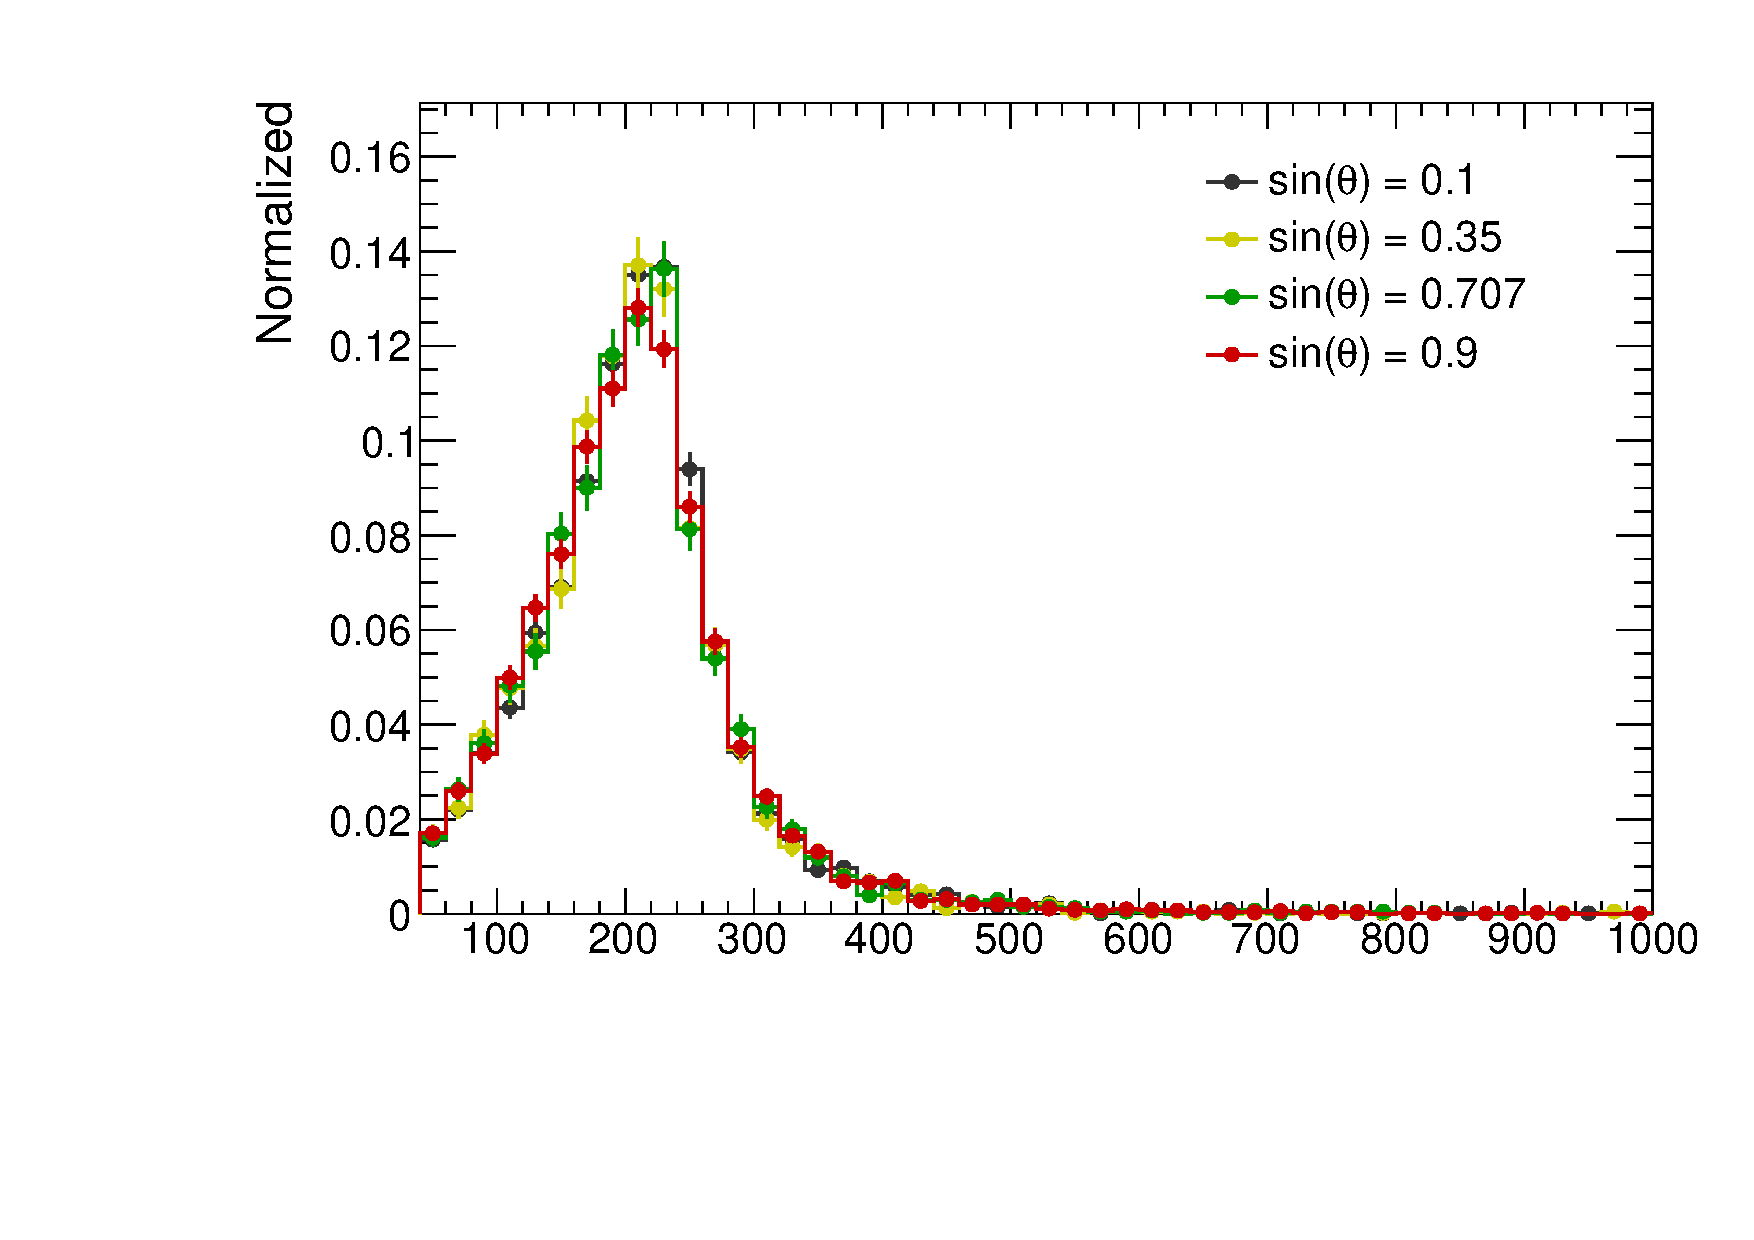
\includegraphics[width=0.48\textwidth]{texinputs/04_grid/figures/monoz/leptonic/SinpScan_mA600_ma250_MET.pdf} 
\caption{\MET distribution after preselection for scans of $\tan{\beta}$ for fixed \mA =600 \GeV and \ma = 150 \GeV (left) and for $\sin{\theta}$ for fixed \mA = 600 \GeV and \ma = 250 \GeV (right).  These parameter have little impact on the event's kinematic distributions, except for small values of \tanb where there is a slight softening and broadening of the \MET distribution caused by the increased contribution from the top box feynman diagram.}
\label{fig:monoz_kin_tanb_sintheta}
\end{figure}


\begin{figure}
\centering
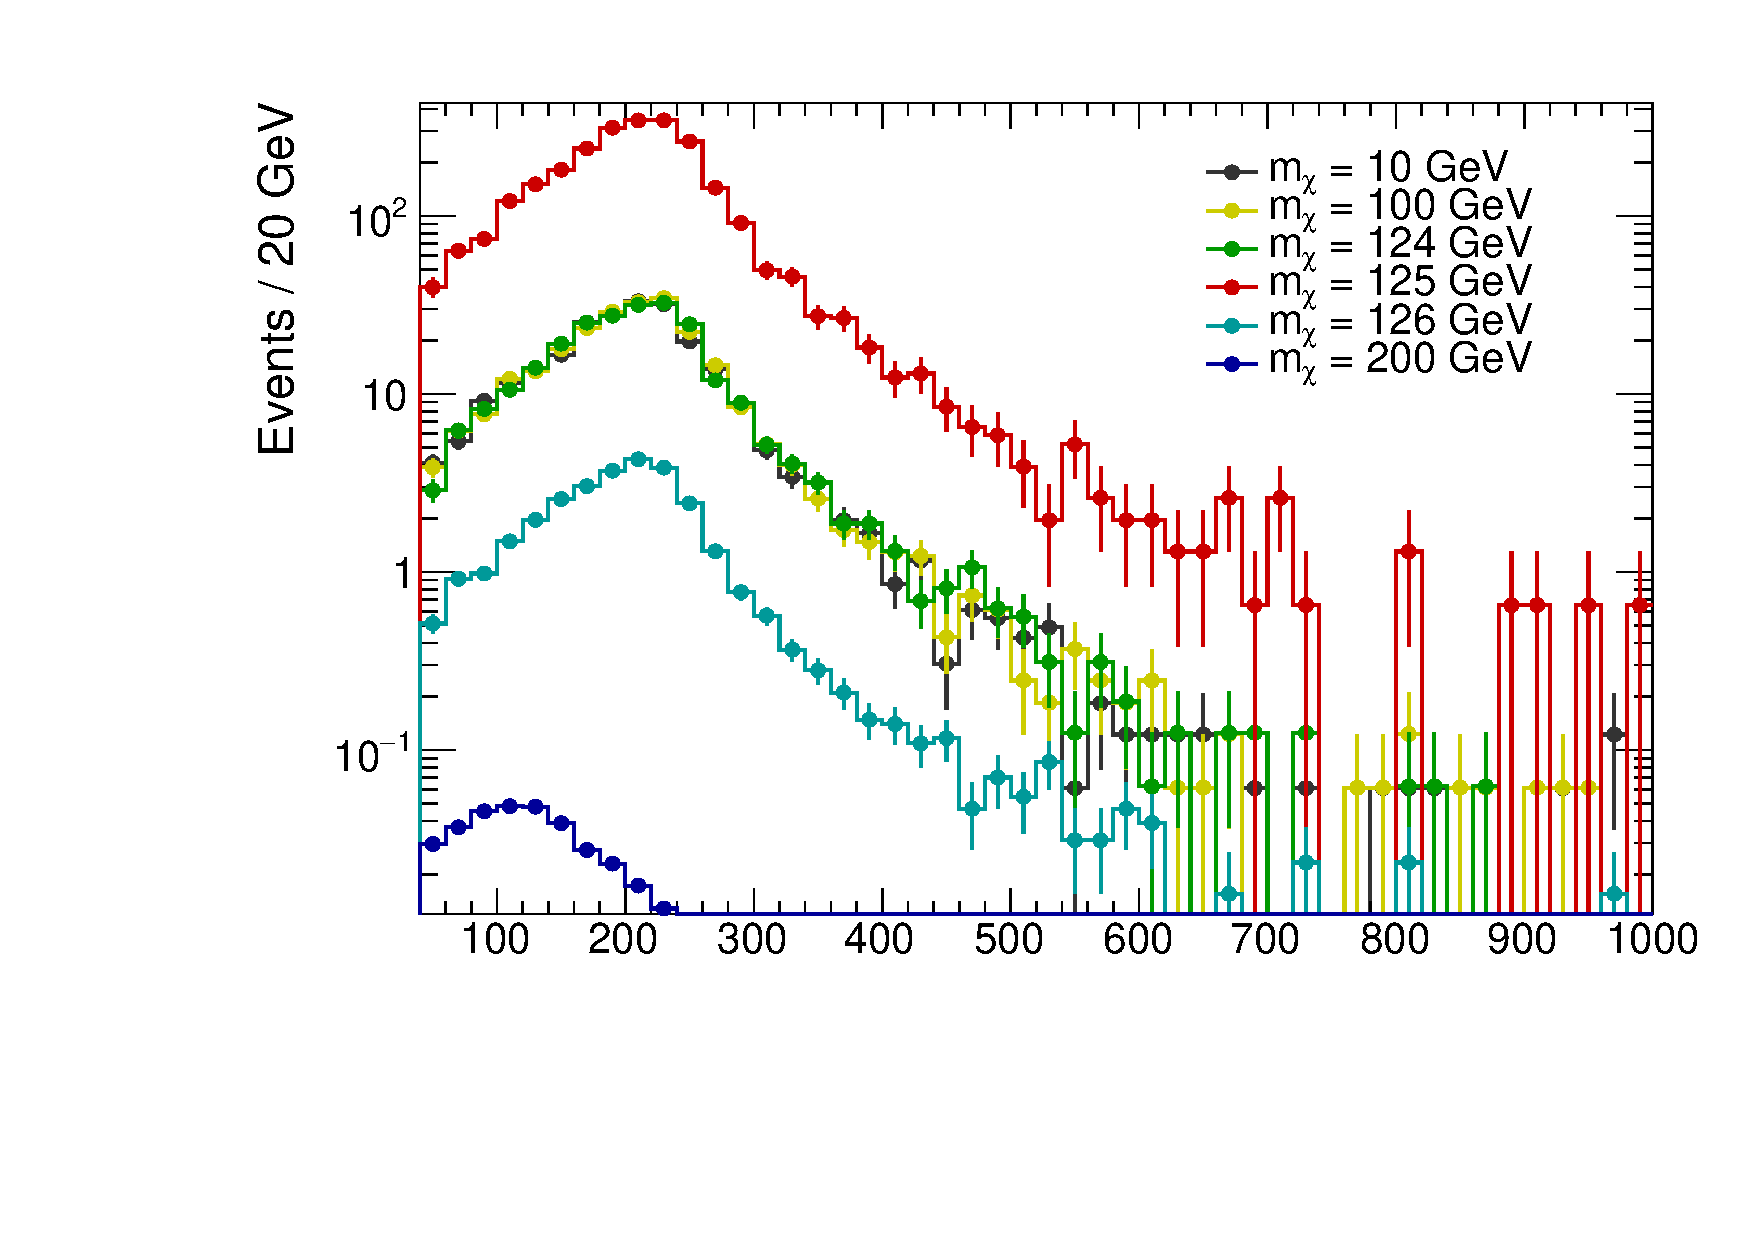
\includegraphics[width=0.48\textwidth]{texinputs/04_grid/figures/monoz/leptonic/mDMScan_mA600_ma250_MET.pdf}
\includegraphics[width=0.47\textwidth]{texinputs/04_grid/figures/monoz/leptonic/mDMScan_ma250.pdf}
\caption{\MET distributions following preselection are shown (left) scaled to 40 \ifb and (right) normalized to unity are shown for different values of \mDM with fixed \mA = 600 \GeV and \ma = 250 \GeV.  In the $\mDM < \frac{\ma}{2}$ region, \mDM has no effect on event yield or \MET distribution, at $\mDM = \frac{\ma}{2}$ a resonant enhancement to the cross section occurs, and in the off-shell region where  $\mDM > \frac{\ma}{2}$ cross section steeply drops.  The \MET shape remains the same up to, and even slightly above, $\mDM = \frac{\ma}{2}$, but further off shell the \MET distribution becomes increasingly disperse.  For \mDM = 200 \GeV, DM can still decay on-shell through the $A$.  For \mDM = 500 \GeV both pseudoscalaras are off-shell and the \MET distribution is without structure.}
\label{fig:dm_scan_ll}
\end{figure}


\begin{figure}
\centering
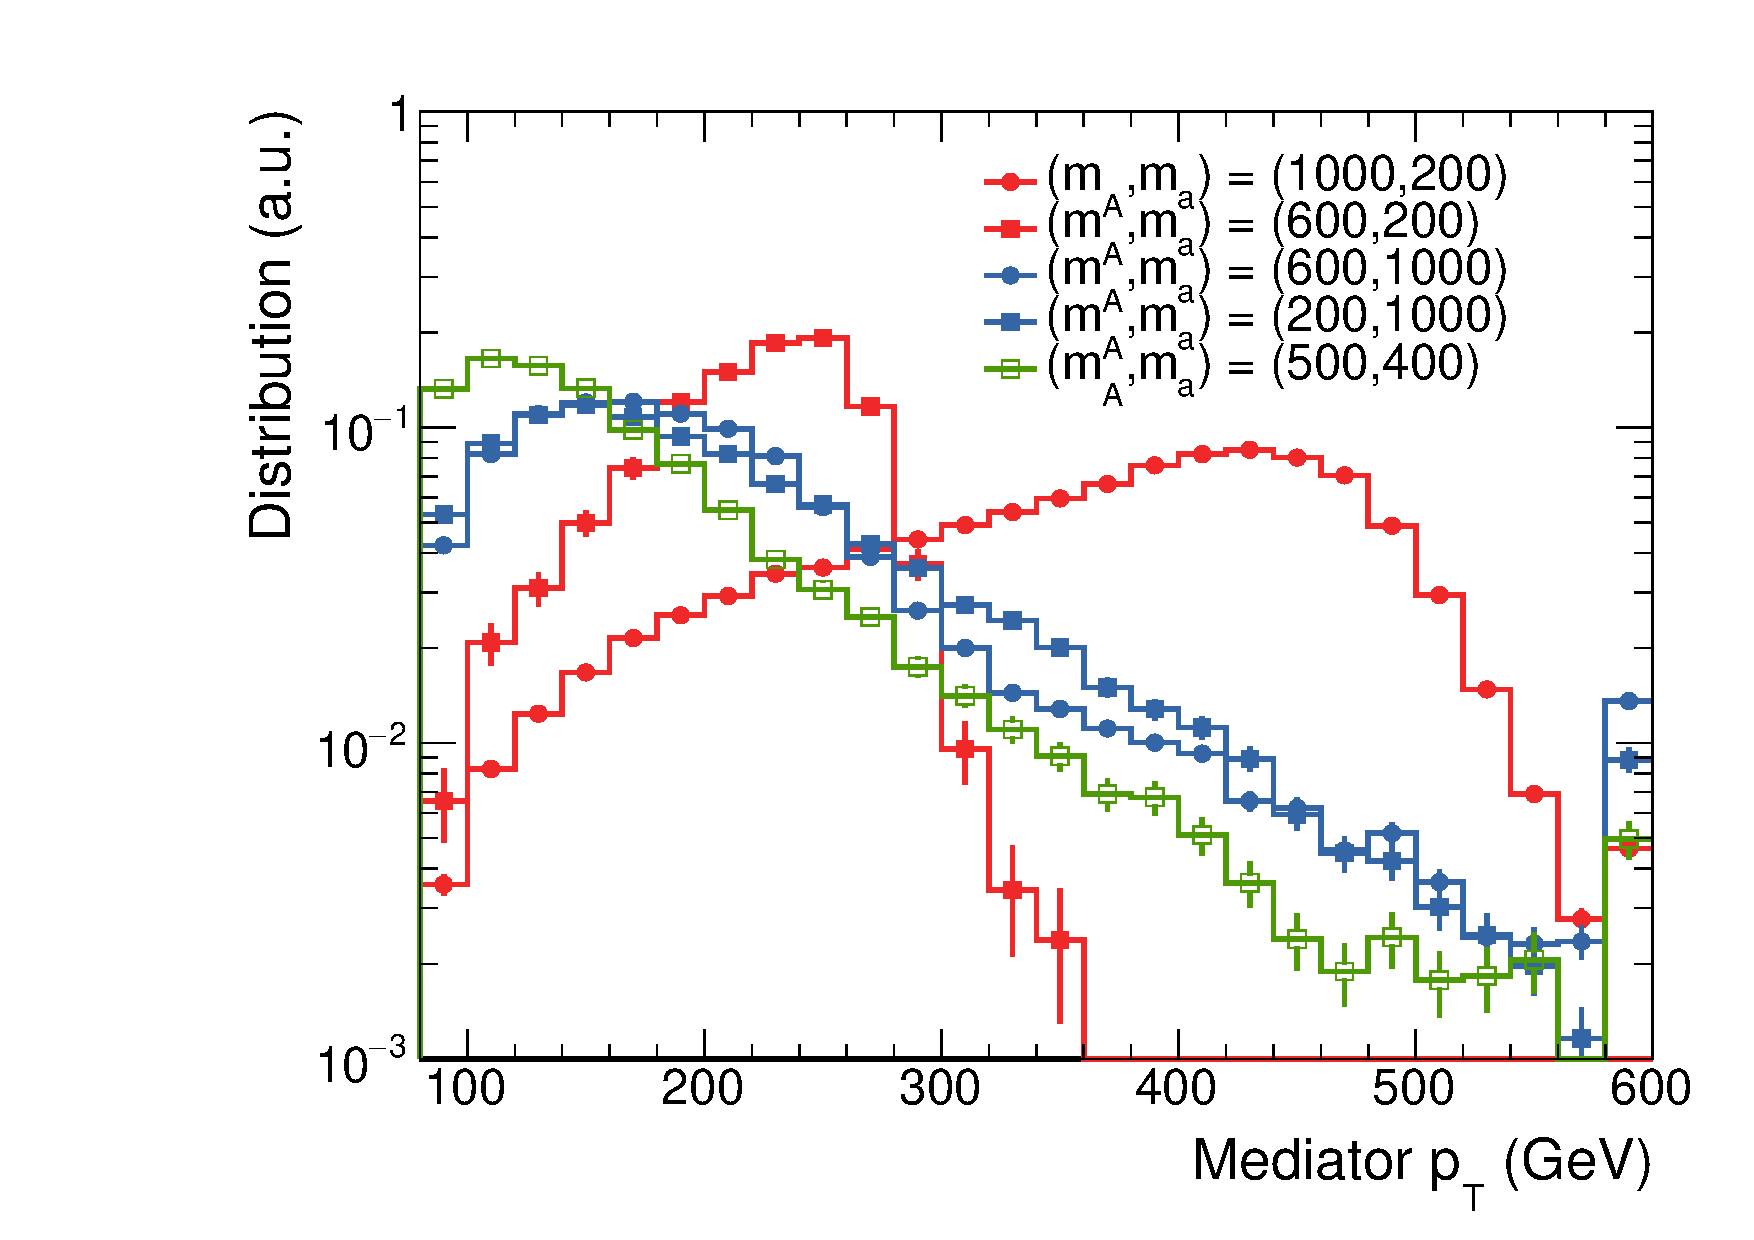
\includegraphics[width=0.45\textwidth]{texinputs/04_grid/figures/monoz/leptonic/dmwg-final_h_pt_med_dm.pdf}
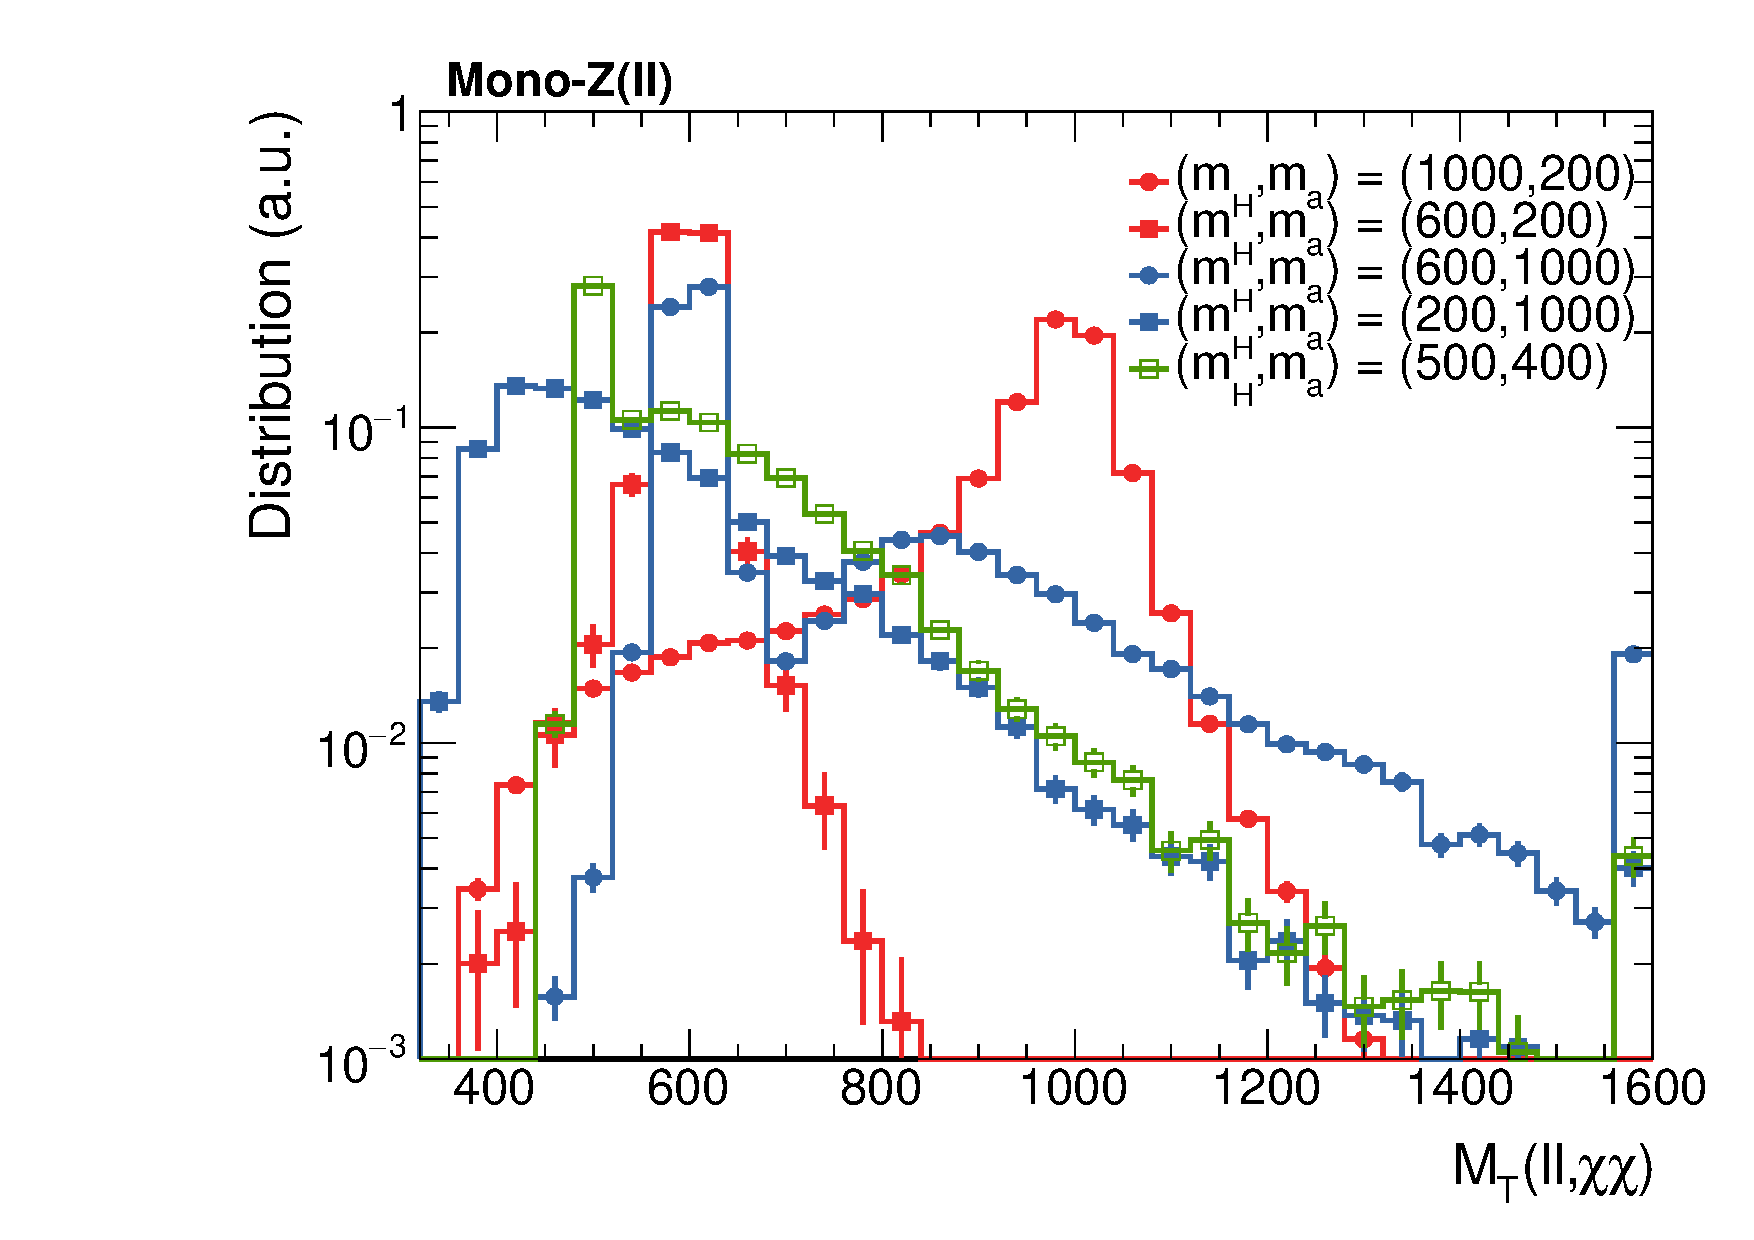
\includegraphics[width=0.45\textwidth]{texinputs/04_grid/figures/monoz/leptonic/dmwg-final_h_mt_total.pdf}
\caption{\MET and  MT distributions in the signal region. The \MET distribution shows a Jacobian structure in the $\mA > \ma$ regime, the location of which strongly depends on $\mA$. In the region of inverted mass hierarchy $\mA < \ma$, the spectrum is less structured and does not fall off as steeply towards higher values. For a small mass splitting of $\ma-\mA\approx M_{Z}$, the spectrum is shifted to much lower values of \MET. The MT distribution allows to access the resonant nature of the process. Clear mass peaks are present for the normal mass hierarchy. In the inverted region, the MT distribution is more sensitive to the mass difference $\ma-\mA$ than the \MET distribution, allowing to differentiate between signal hypotheses that give near-identical \MET distributions. }
\label{fig:monoz_kin_final}
\end{figure}


\begin{figure}
\centering
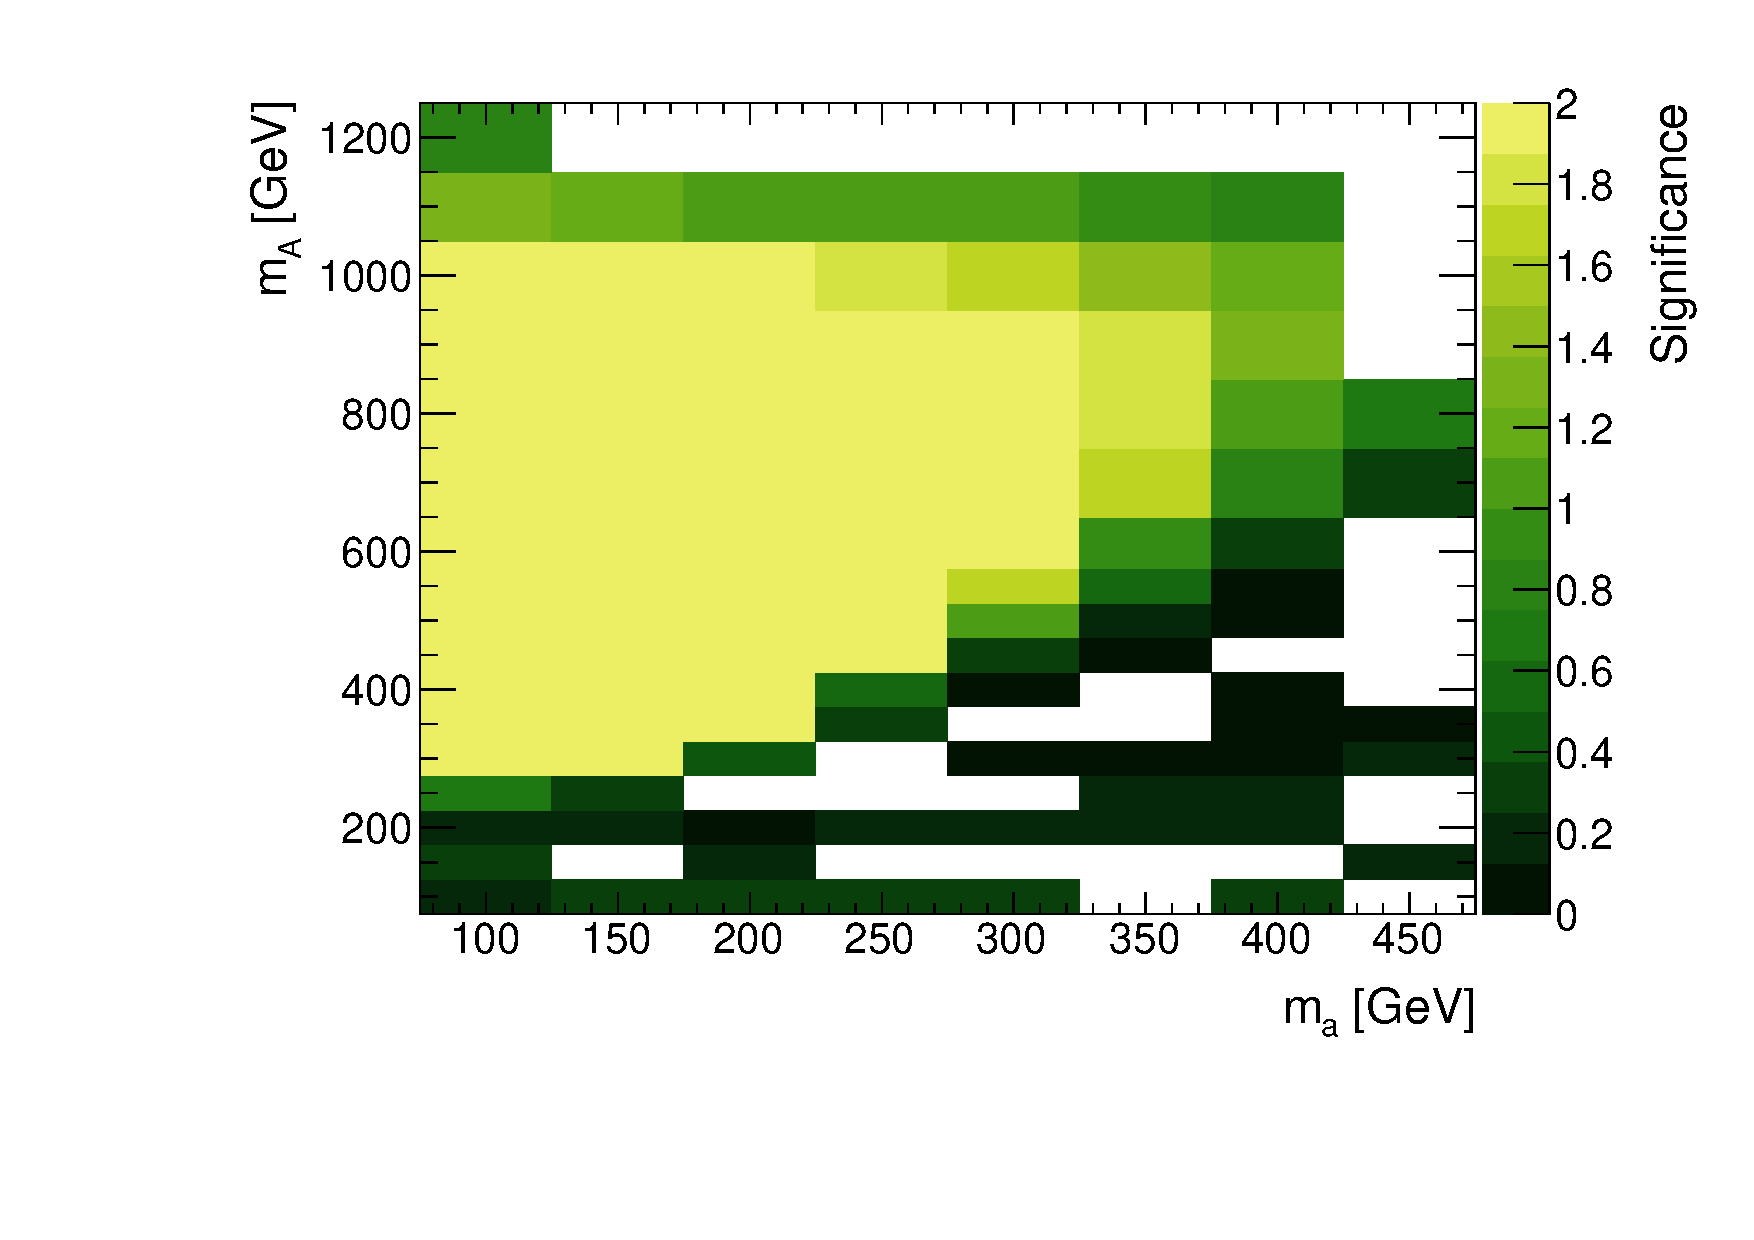
\includegraphics[width=0.9\textwidth]{texinputs/04_grid/figures/monoz/leptonic/mAma_Significance_ll.pdf}
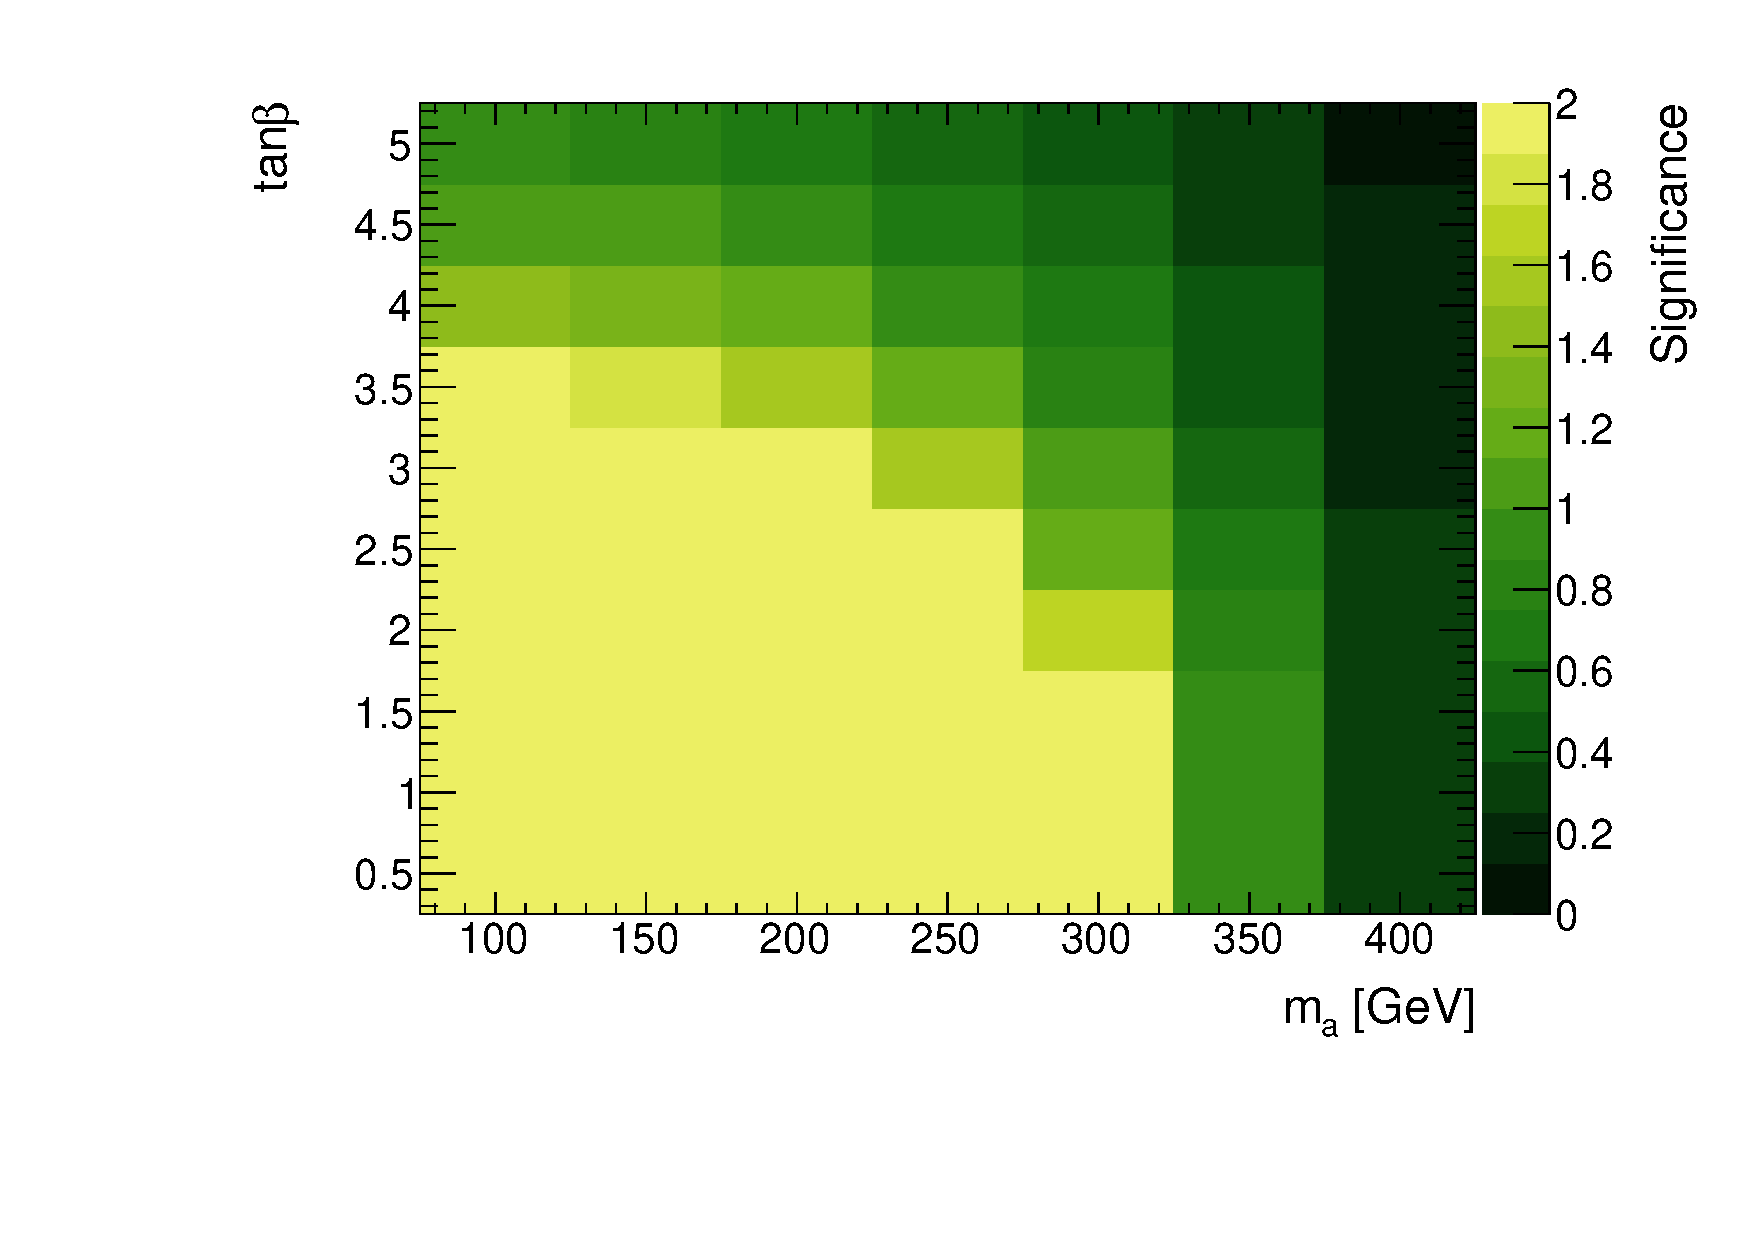
\includegraphics[width=0.9\textwidth]{texinputs/04_grid/figures/monoz/leptonic/tanbma_Significance_ll.pdf}
\caption{Expected significances are calculated using published background estimates and assuming a reconstruction efficiency of 75\%.  The ATLAS and CMS experiments are expected to be sensitive to regions with significances greater than 2.}
\label{fig:expected_significance_monozll}
\end{figure}


\FloatBarrier
\subsection{Studies of the mono-Z (hadronic) signature}
\begin{figure}
\centering
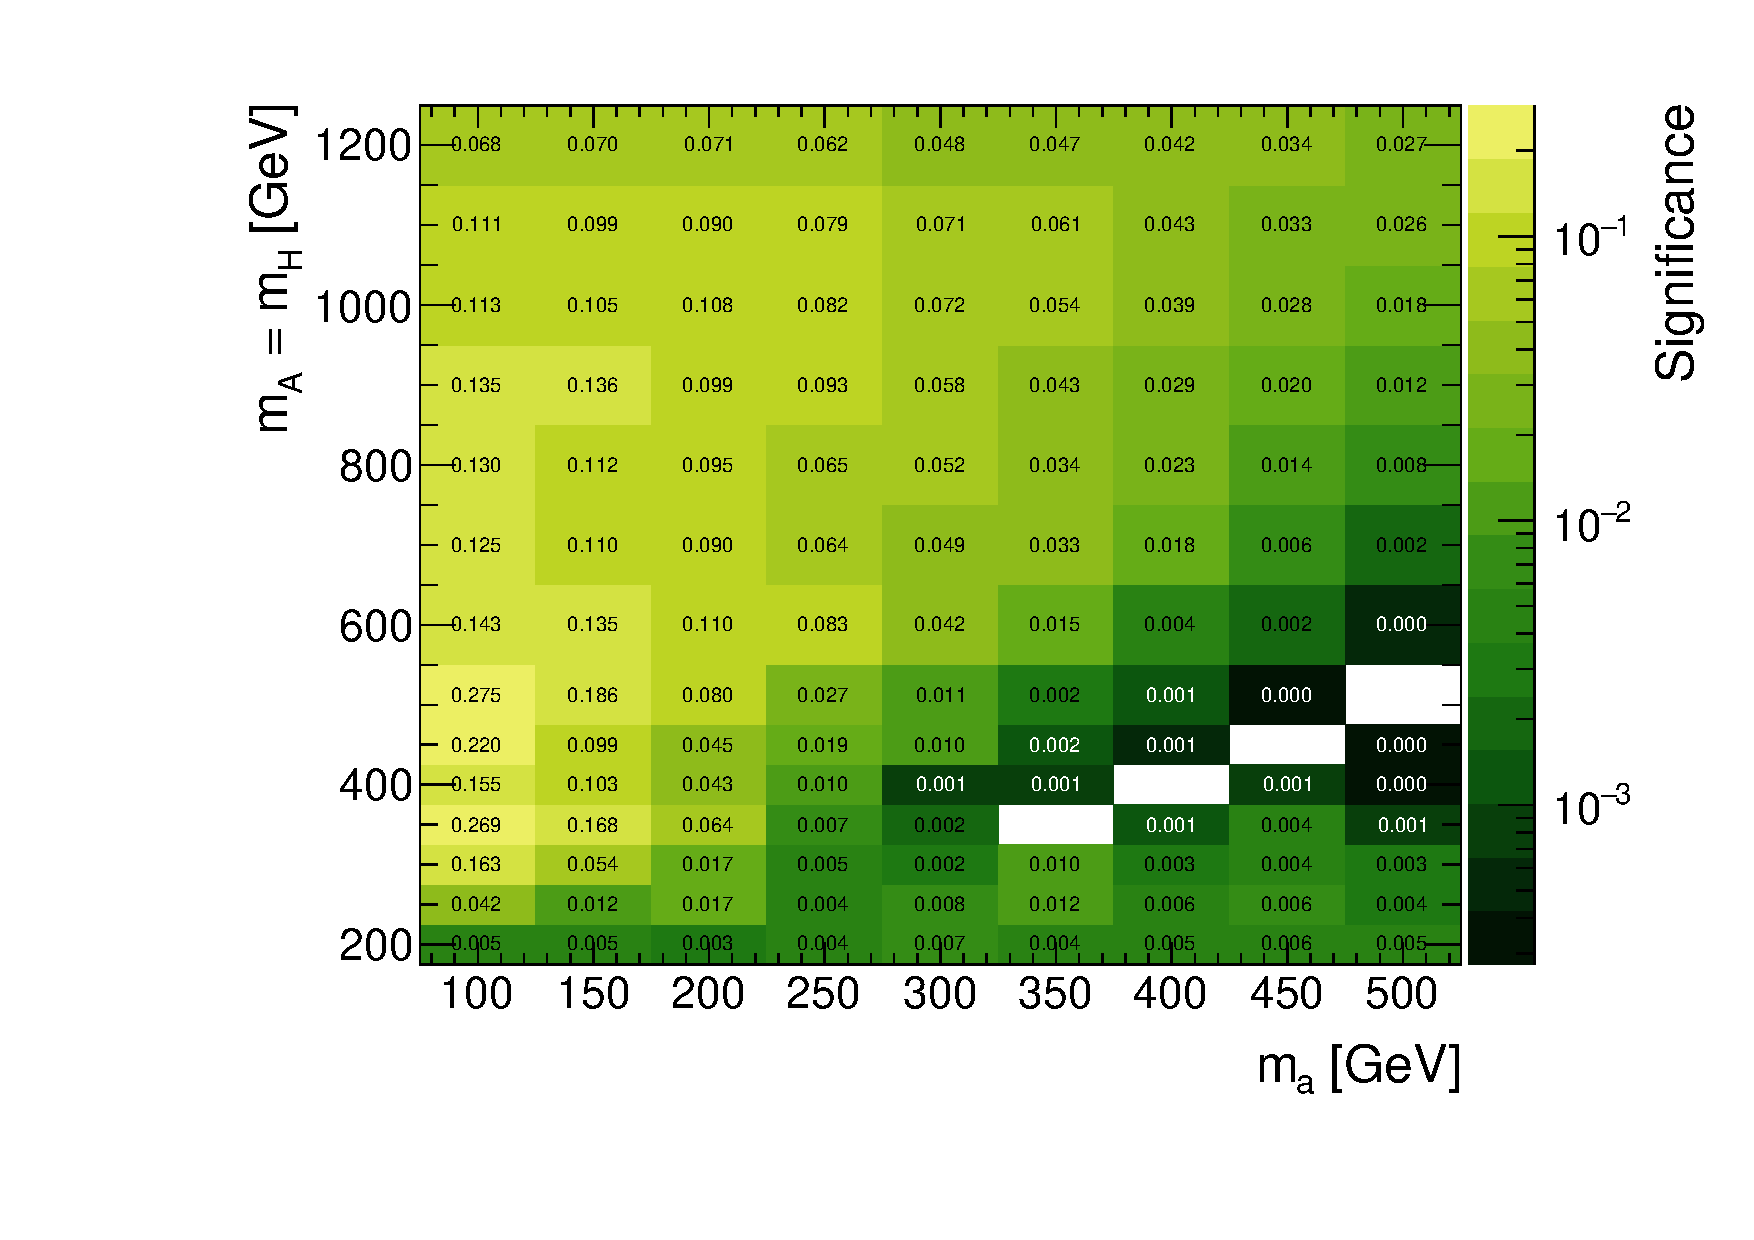
\includegraphics[width=0.45\textwidth]{texinputs/04_grid/figures/monoz/hadronic/grid_mA_ma_resl_bin100_sign_type3_bkg_uncert_0p10.pdf}
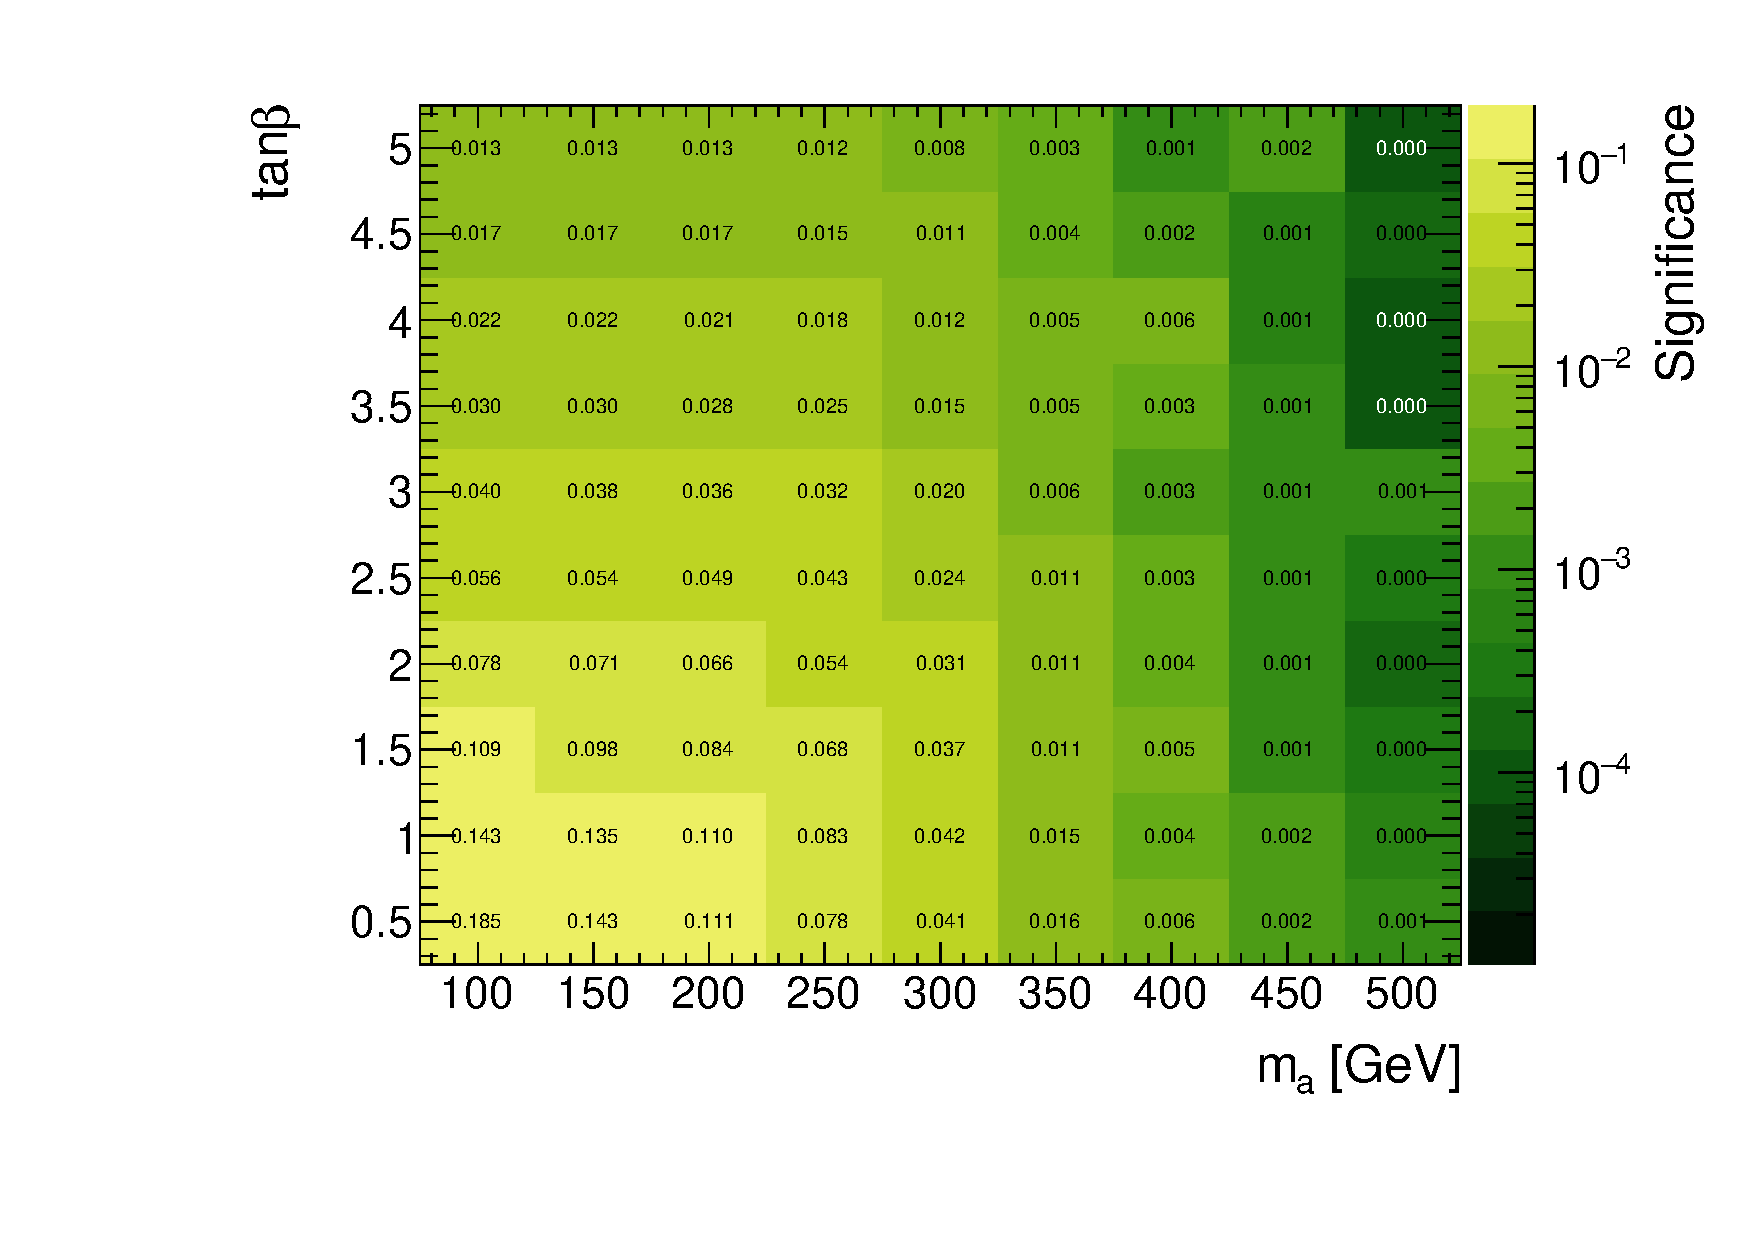
\includegraphics[width=0.45\textwidth]{texinputs/04_grid/figures/monoz/hadronic/grid_tanb_ma_resl_bin100_sign_type3_bkg_uncert_0p10.pdf}
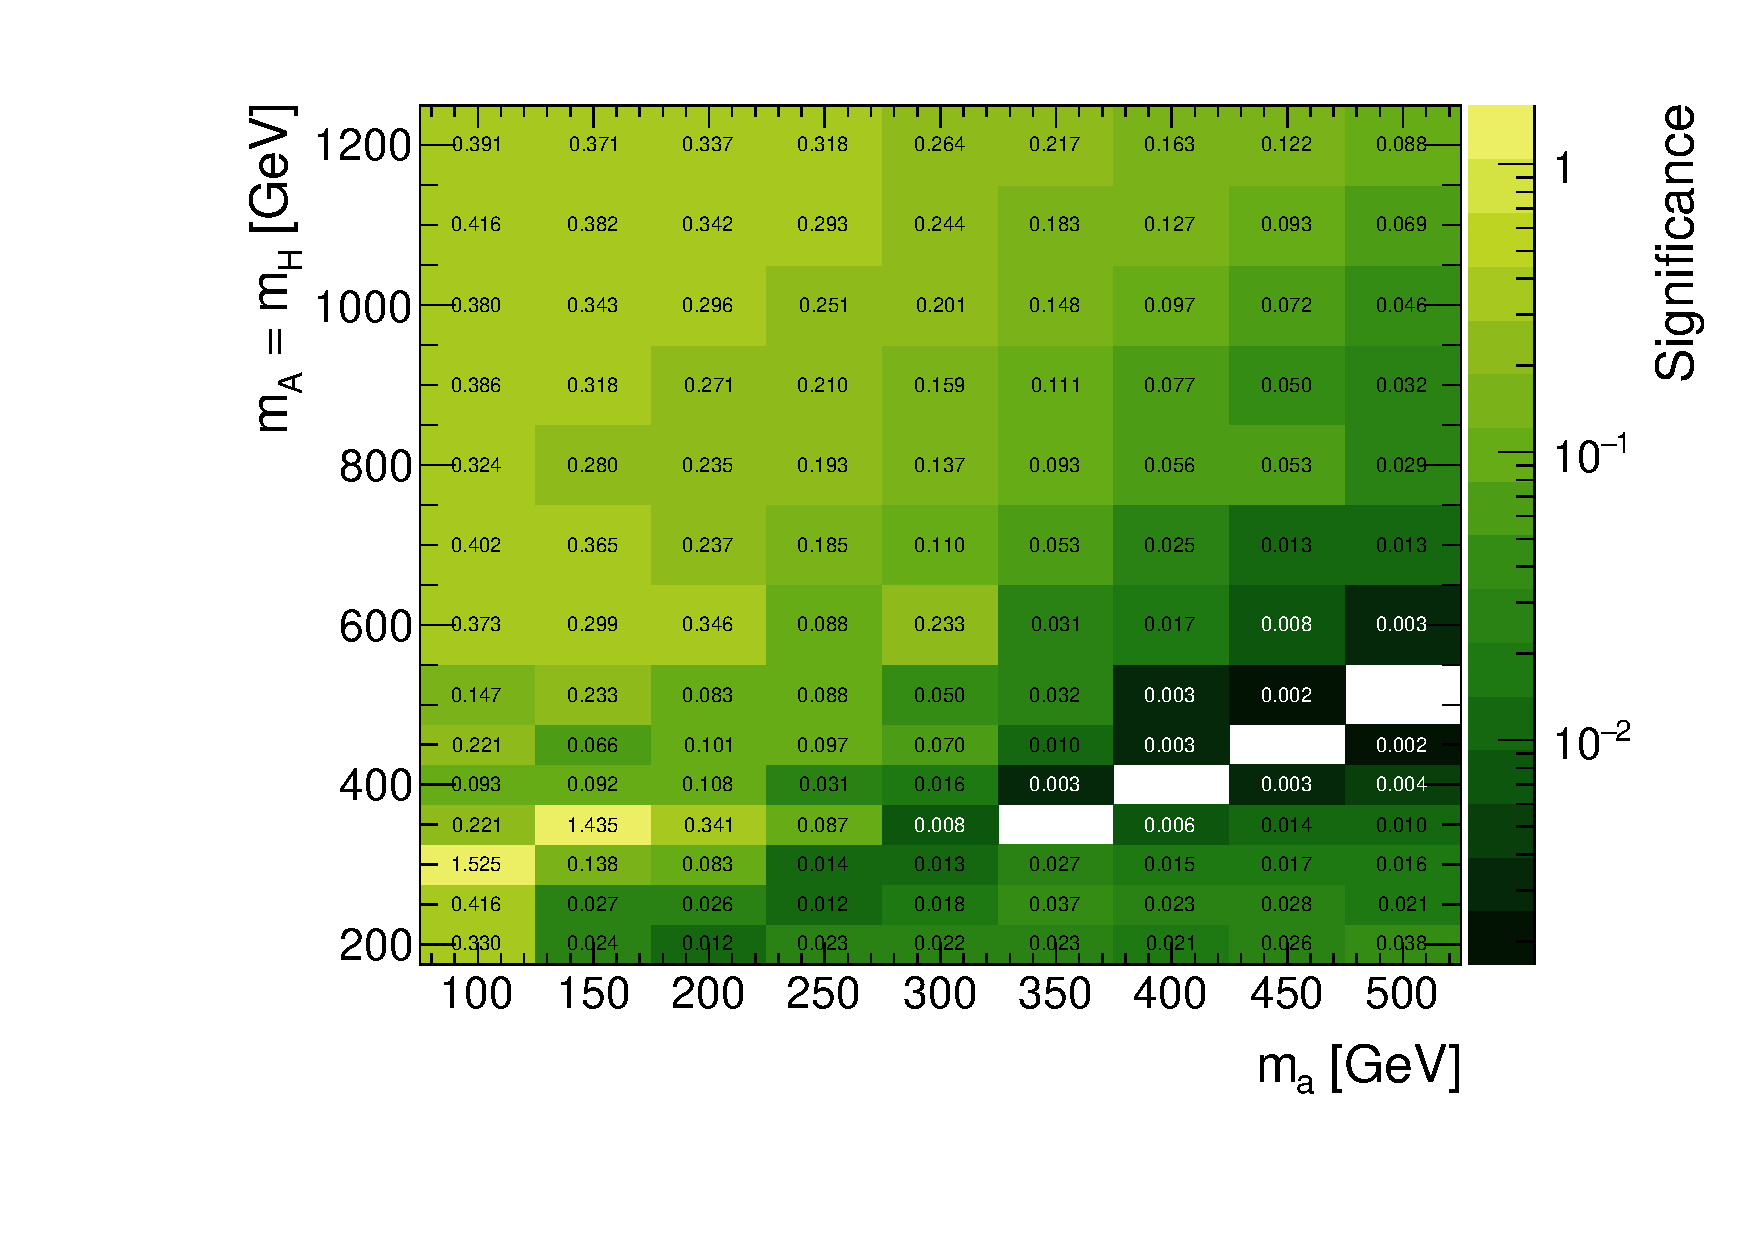
\includegraphics[width=0.45\textwidth]{texinputs/04_grid/figures/monoz/hadronic/grid_mA_ma_merged_bin100_sign_type3_bkg_uncert_0p10.pdf}
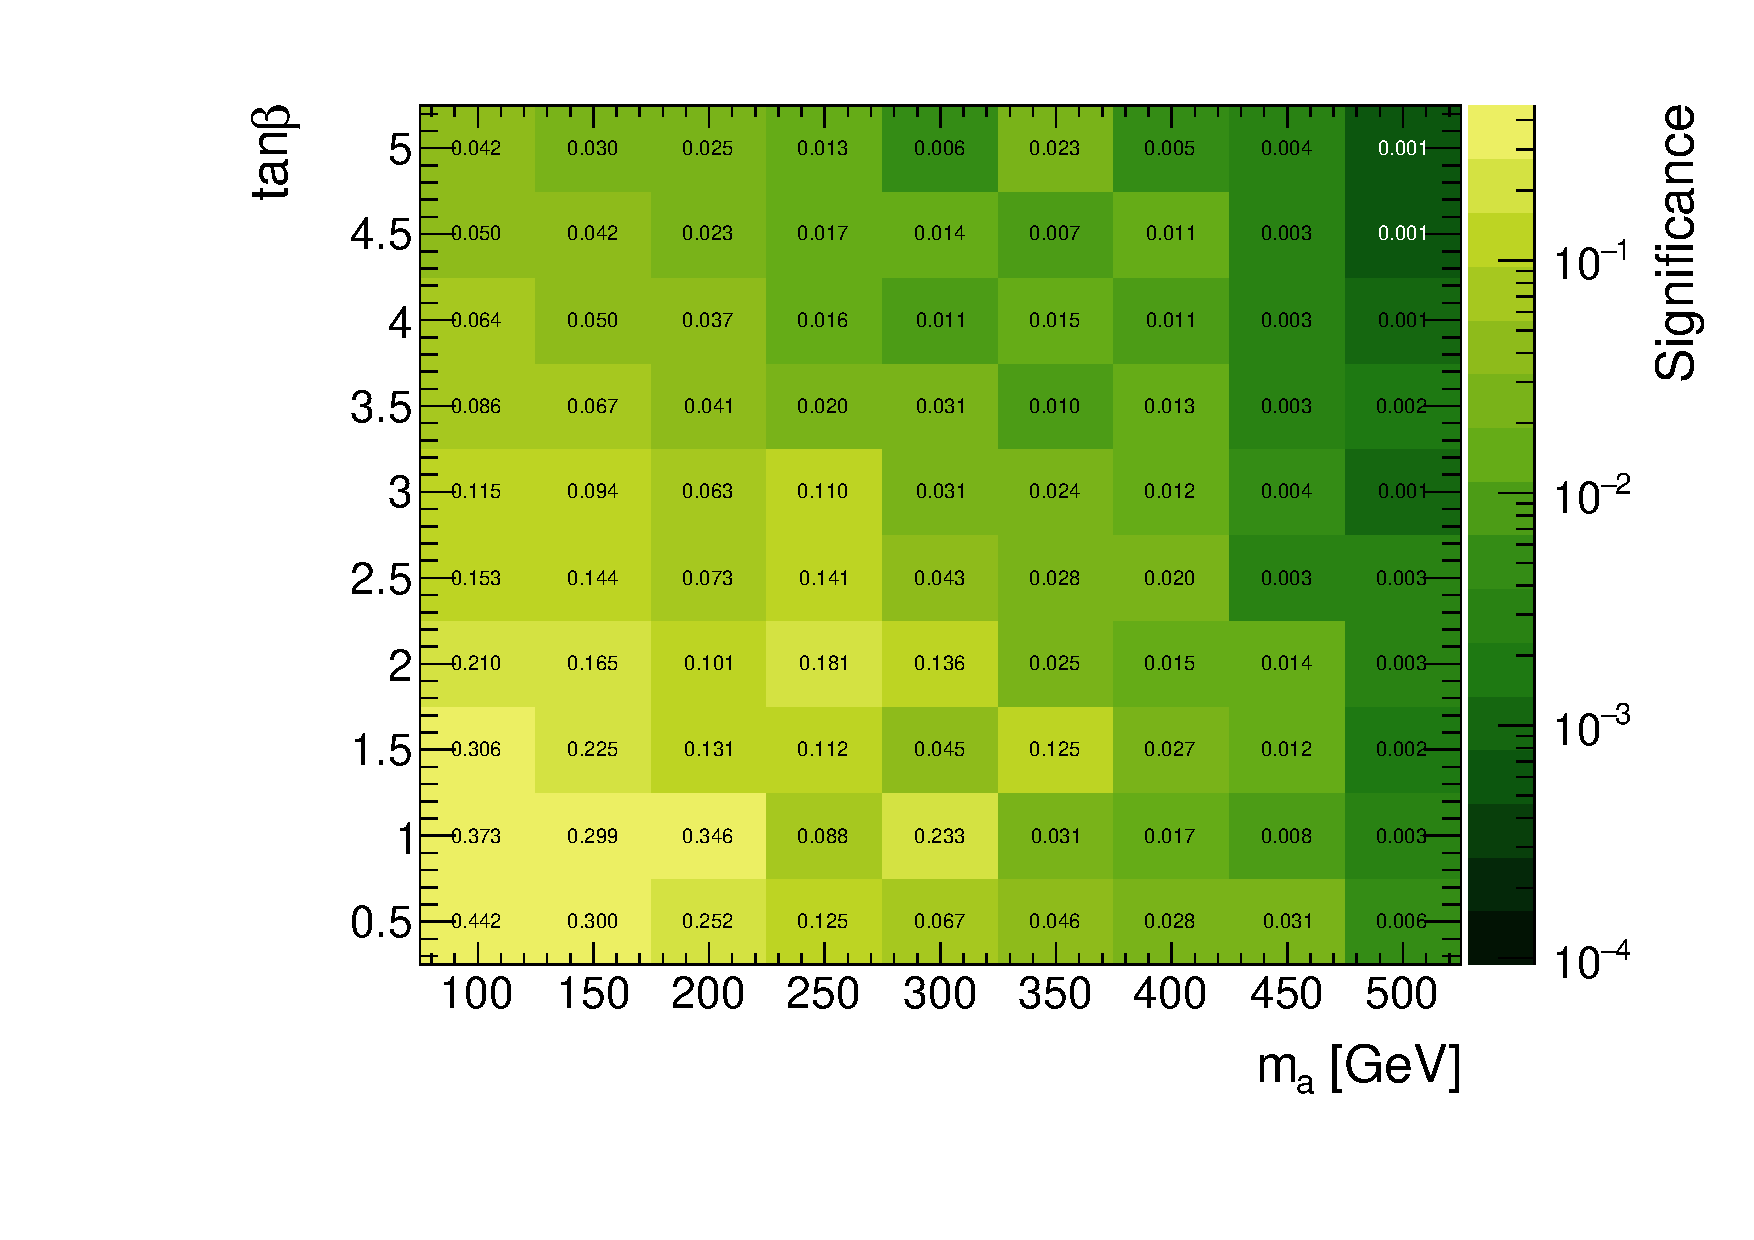
\includegraphics[width=0.45\textwidth]{texinputs/04_grid/figures/monoz/hadronic/grid_tanb_ma_merged_bin100_sign_type3_bkg_uncert_0p10.pdf}
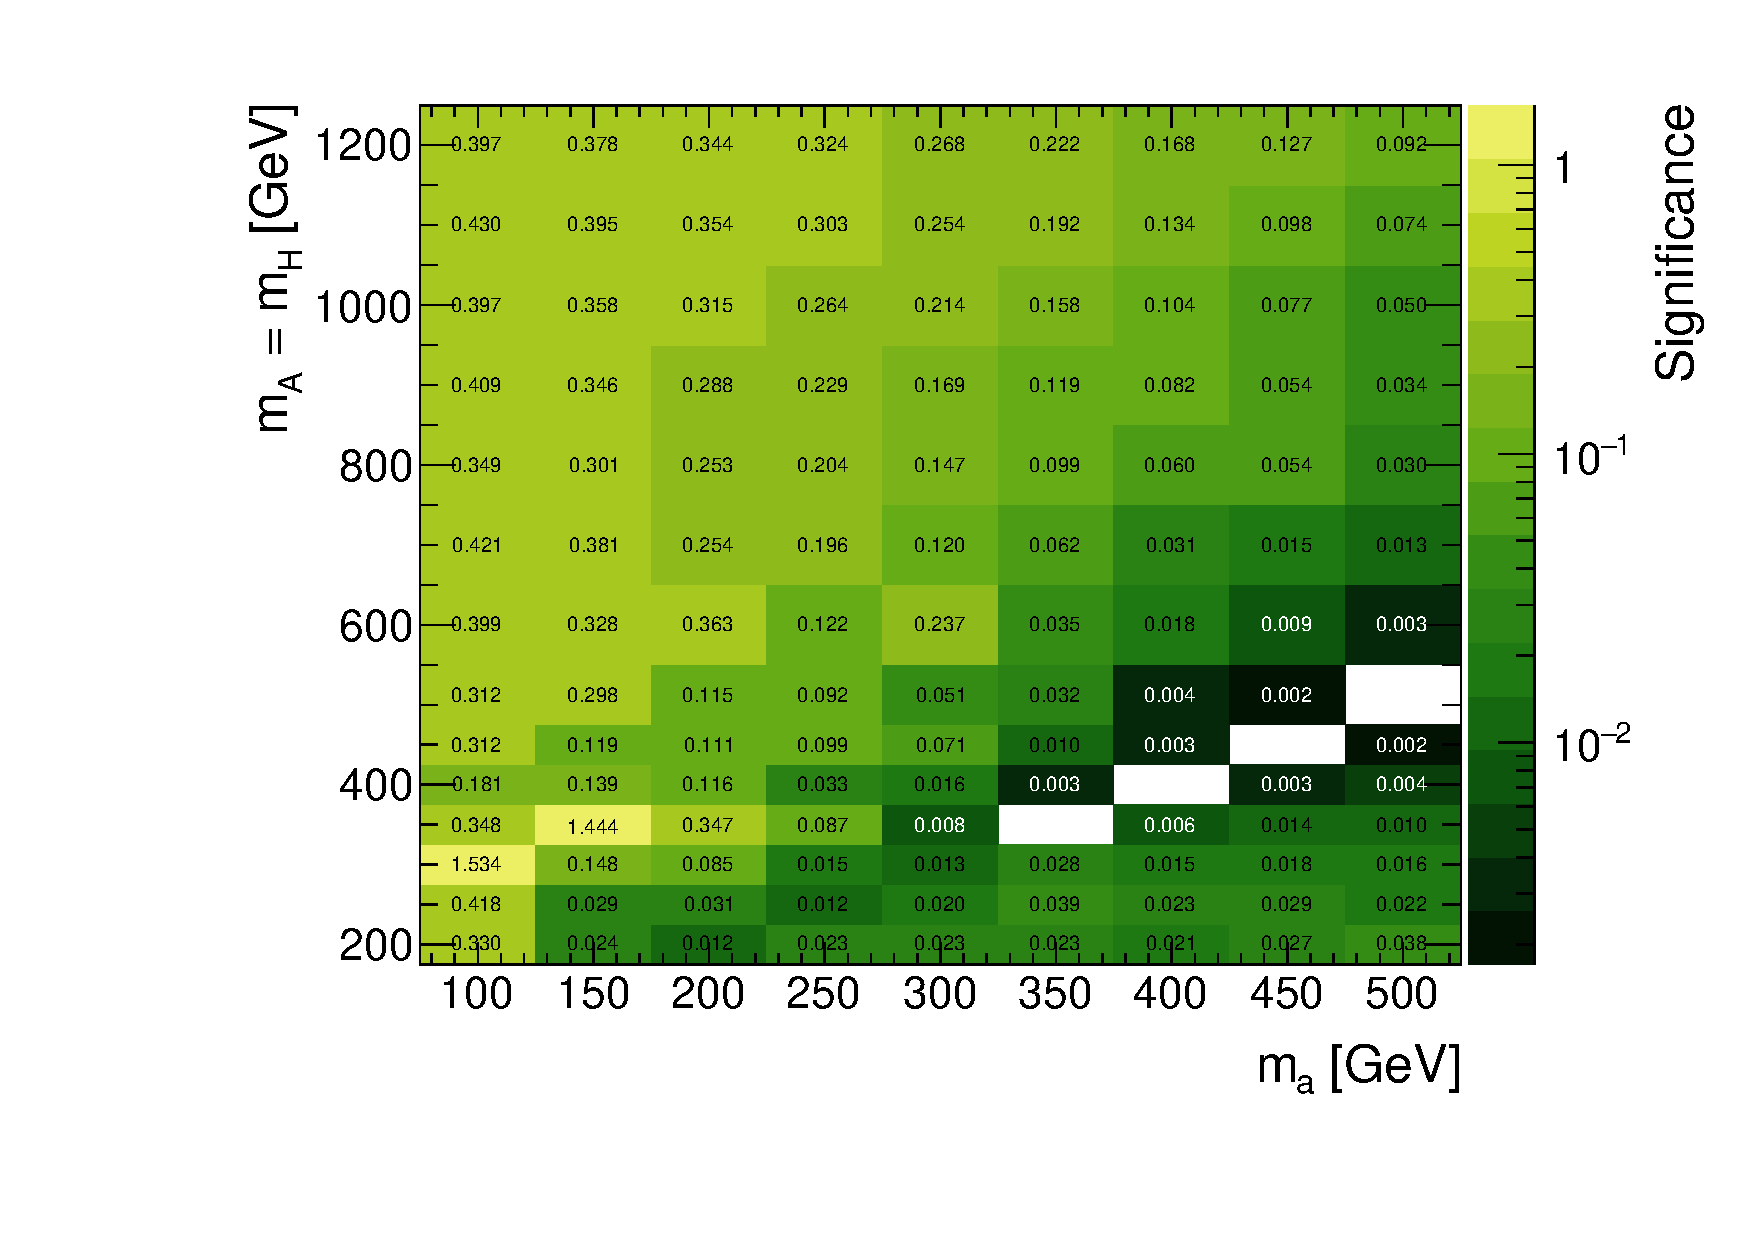
\includegraphics[width=0.45\textwidth]{texinputs/04_grid/figures/monoz/hadronic/grid_mA_ma_sum_bin100_sign_type3_bkg_uncert_0p10.pdf}
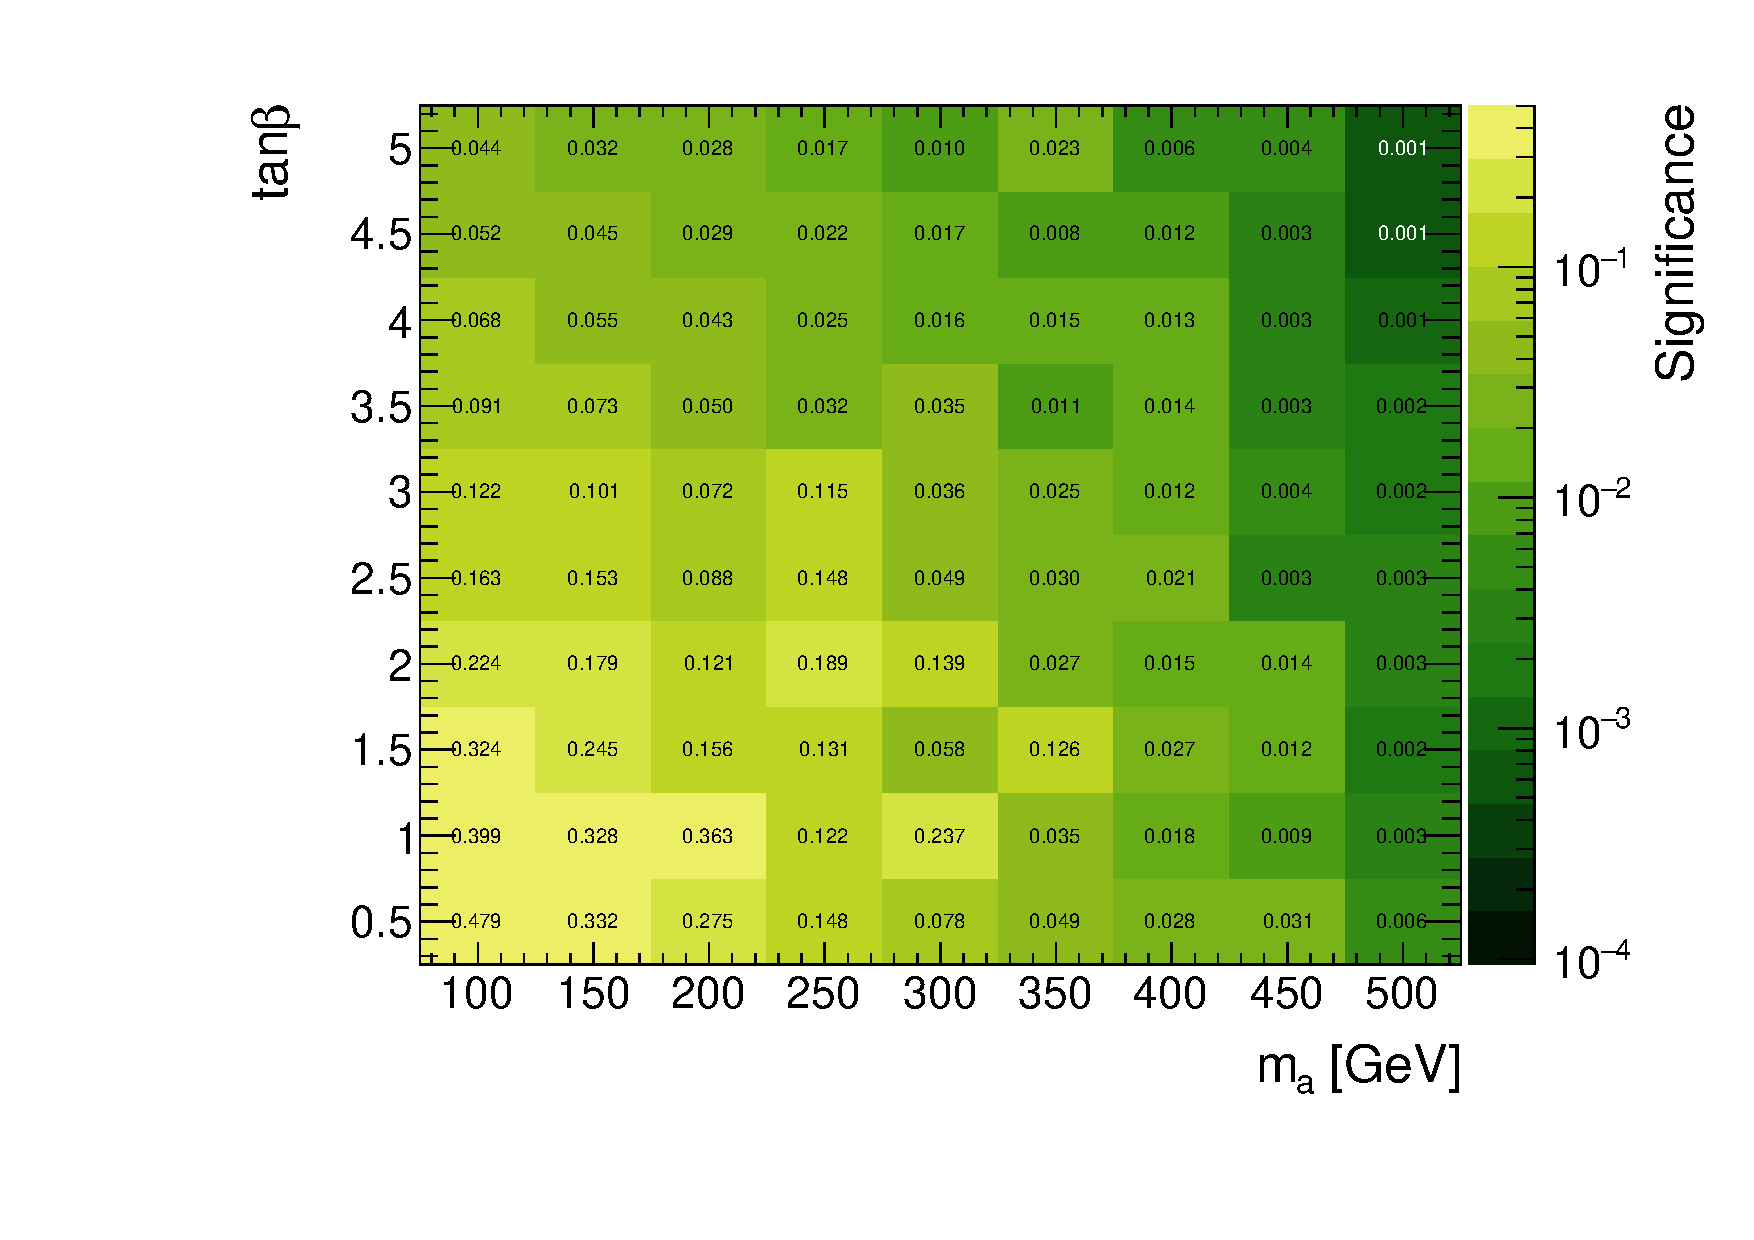
\includegraphics[width=0.45\textwidth]{texinputs/04_grid/figures/monoz/hadronic/grid_tanb_ma_sum_bin100_sign_type3_bkg_uncert_0p10.pdf}
\caption{Significance (as defined in the text) for the mono-$Z$ hadronic events 
$pp \rightarrow Z(\to q\bar{q})\chi\overline{\chi}$ in the \ma vs \mA (left) and \ma vs $\tan\beta$ (right) grids. 
Shown at the top, middle and bottom are the resolved only, boosted only and the combined resolved+boosted 
analysis, respectively.}
\label{fig:monozhad_significance_grid}
\end{figure}

The sensitivity of the resolved, boosted and the combined analysis selections to the mono-$Z$ hadronic signature 
is examined. The main background for this signature is $Z \to \nu\nu$ events in association with jets. 
The sample of $Z (\to \nu\nu)$+jets events is produced using Sherpa~2.2.1 and the matrix elements are calculated
up to 2 partons at next-to-leading order and up to 4 partons at leading order. The $Z (\to \nu\nu)$+jets events
are analyzed at particle level with the same criteria used for the signal. The number of $Z \to \nu\nu$ events 
after applying the cuts is increased by a factor 2 to account for the contribution from other backgrounds. 
This factor is chosen from the 
ATLAS dark matter search in the mono-$Z$ hadronic signature using 3.2~fb$^{-1}$ of 13~TeV data,
published in Ref.~\ref{EXOT-2015-08}. The sensitivity is defined in this study as 
%
\begin{equation}
\text{Significance} = \sqrt{\sum_{\text{bin}} Z_{\text{bin}}^2}
\label{eq:monozhad_sig}
\end{equation}
%
where the per-bin significance, $Z_{\text{bin}}$, is obtained, using asymptotic calculation of the 
Poisson likelihood ratio statistic, to be 
%
\begin{equation}
Z_{\text{bin}} = \left[ 2\left( (s+b)\ln \left[ \frac{(s+b)(b+\sigma_b^2)}{b^2+(s+b)\sigma_b^2} \right] - \frac{b^2}{\sigma_b^2} \ln \left[ 1+\frac{\sigma_b^2 s}{b(b+\sigma_b^2)} \right] \right) \right]^{1/2} 
\end{equation}
%
with the assumption of 10\% background uncertainty in each \MET bin. 
The sum in Eq.(\ref{eq:monozhad_sig}) is taken over all \MET bins after applying the final selections.
The results are shown in Fig.~\ref{fig:monozhad_significance_grid} for the resolved only, booted only and 
the combined resolved+boosted analysis selections, corresponding to the integrated luminosity of 40~fb$^{-1}$
at $\sqrt{s} = 13$~TeV. The significance depends strongly on the assumption of background uncertainty 
since a large number of background events remain in this simple analysis with a minimum set of selection criteria.
More realistic analysis performed in LHC experiments is expected to improve the sensitivity.



\subsubsection{Studies of DM+heavy flavor signature}
%% \documentclass[11pt]{article}
%% \usepackage{graphicx,epsfig}

%% % Shorthand for \phantom to use in tables
%% \newcommand{\pho}{\phantom{0}}
%% \newcommand{\BibTeX}{\textsc{Bib\TeX}}
%% \newcommand{\File}[1]{\texttt{#1}\xspace}
%% \newcommand{\Macro}[1]{\texttt{\textbackslash #1}\xspace}
%% \newcommand{\Option}[1]{\textsf{#1}\xspace}
%% \newcommand{\Package}[1]{\texttt{#1}\xspace}
%% \newcommand{\MADGRAPH}{\textsc{MadGraph}}
%% \newcommand{\PYTHIA}{\textsc{Pythia}}

%% \usepackage{subcaption}
%% \usepackage{siunitx}
%% \newcommand{\ttbar}{\ensuremath{\bar{t}t}}
%% \newcommand{\bbbar}{\ensuremath{\bar{b}b}}
%% \newcommand*{\TeV}{\ensuremath{\text{Te\kern -0.1em V}}}
%% \newcommand*{\GeV}{\ensuremath{\text{Ge\kern -0.1em V}}}
%% \newcommand{\pt}{\ensuremath{p_{\mathrm T}}}
%% \newcommand{\met}{\ensuremath{E_{\mathrm T}^{\mathrm miss}}}
%% \usepackage{biblatex}
%% \bibliography{draft}

%% \usepackage{lineno}
%% \linenumbers



%% \begin{document}


Heavy flavour final state have sizeable contributions to the production of the CP-even and CP-odd scalar mass eigenstates, due to the Yukawa structure 
of the couplings in the matter sector. 
In the following sections,  the most important signatures involving either visible or invisible decays of the heavy Higgses are reviewed. 


%%%%-----------------------------------------------------------------------------------------
%%%%-----------------------------------------------------------------------------------------
\subsubsection{Scanning the parameter space}

\paragraph{Scan of $\tan\beta$ and $\sin\theta$:}

\begin{figure}
  \centering
  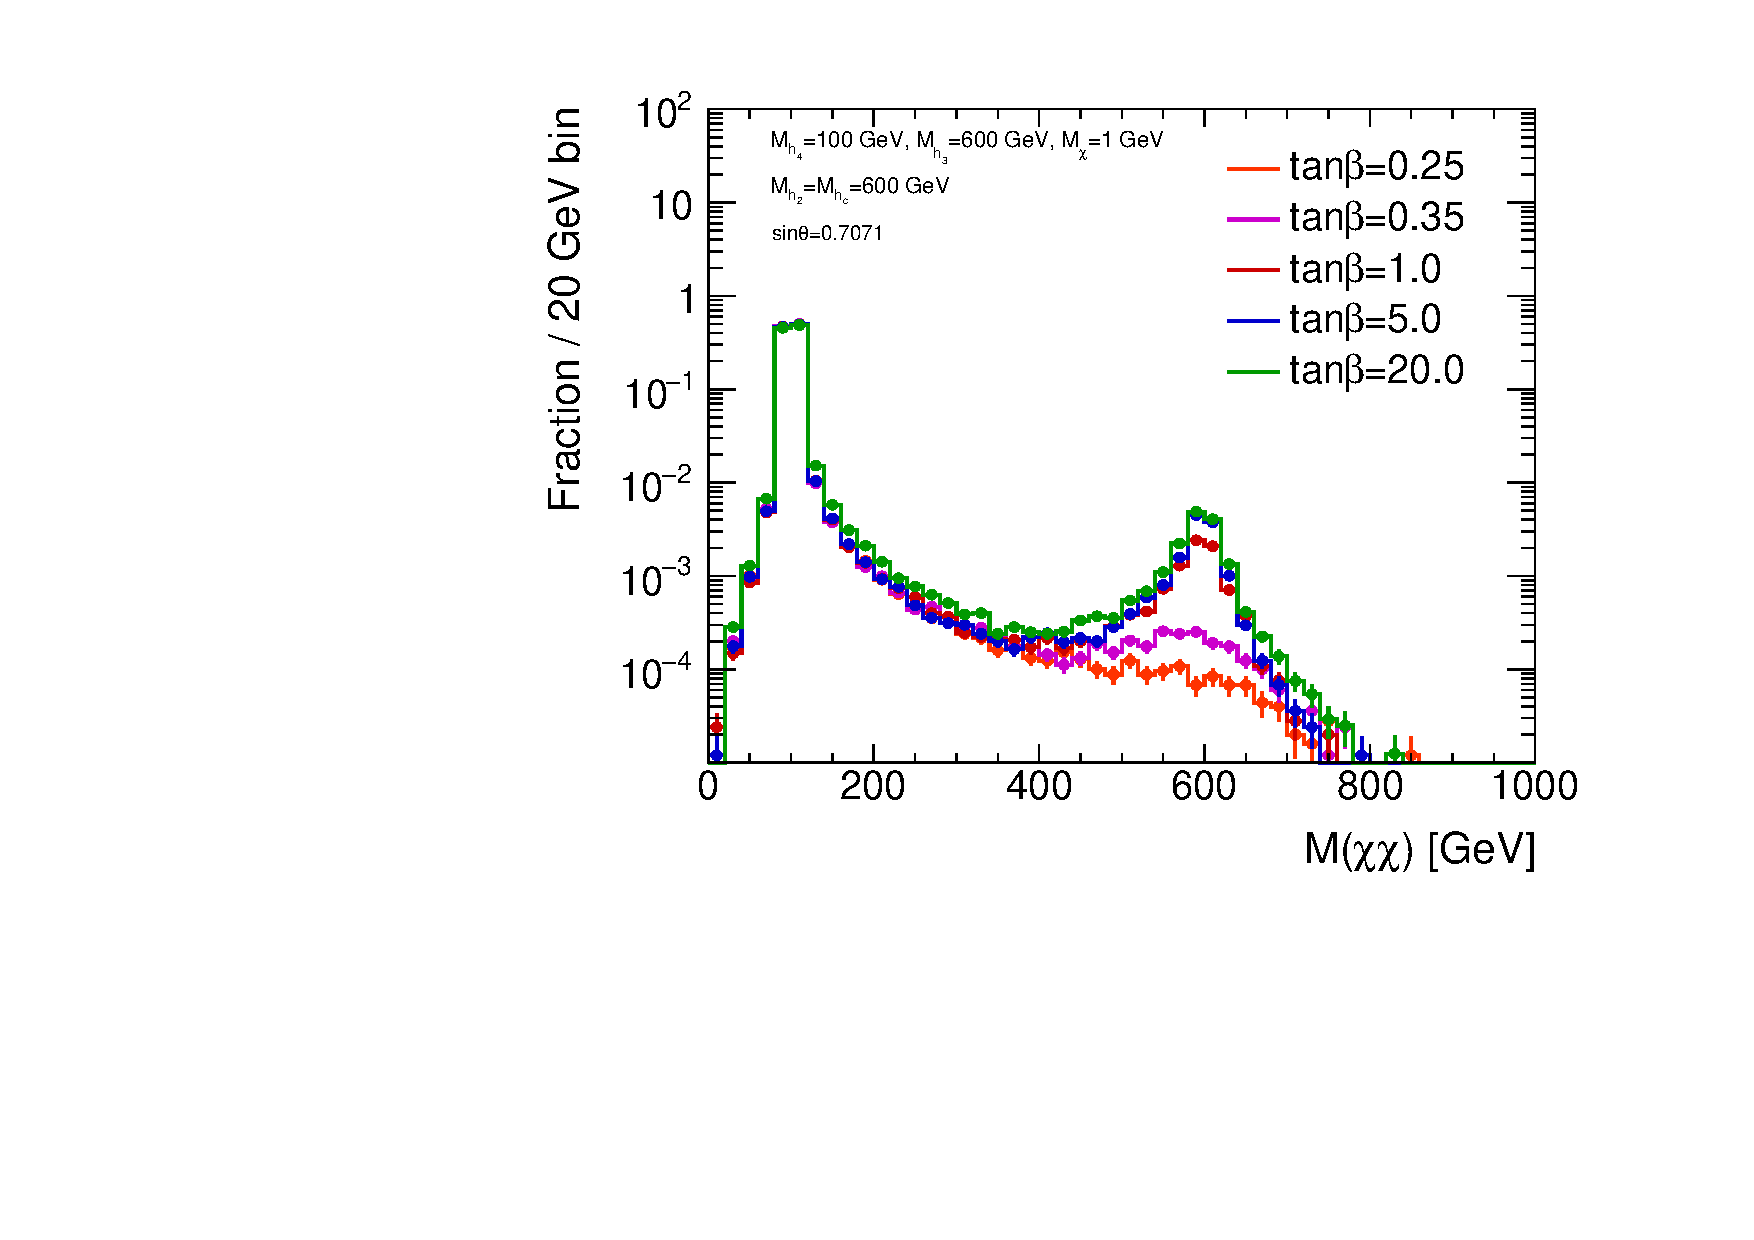
\includegraphics[width=0.6\textwidth]{texinputs/04_grid/figures/DMHF/benchmarking/MDM_1_Ma_100_MA_600_sinp_0.7071_SCAN_tanb_decayed/mchichi.pdf}
  \caption{The mass distribution of the $\chi \bar{\chi}$ system for various values of $\tan\beta$, with $\mathrm{M_a}=100$ GeV, $\mathrm{M_A}=600$ GeV, $\mathrm{M_H}=\mathrm{M_{H^{\pm}}}=600$ GeV, and $\sin\theta=0.7071$.}
  \label{fig:mchichi_tanB}
\end{figure}

\begin{figure}
  \centering
  \begin{subfigure}[b]{0.49\textwidth}
    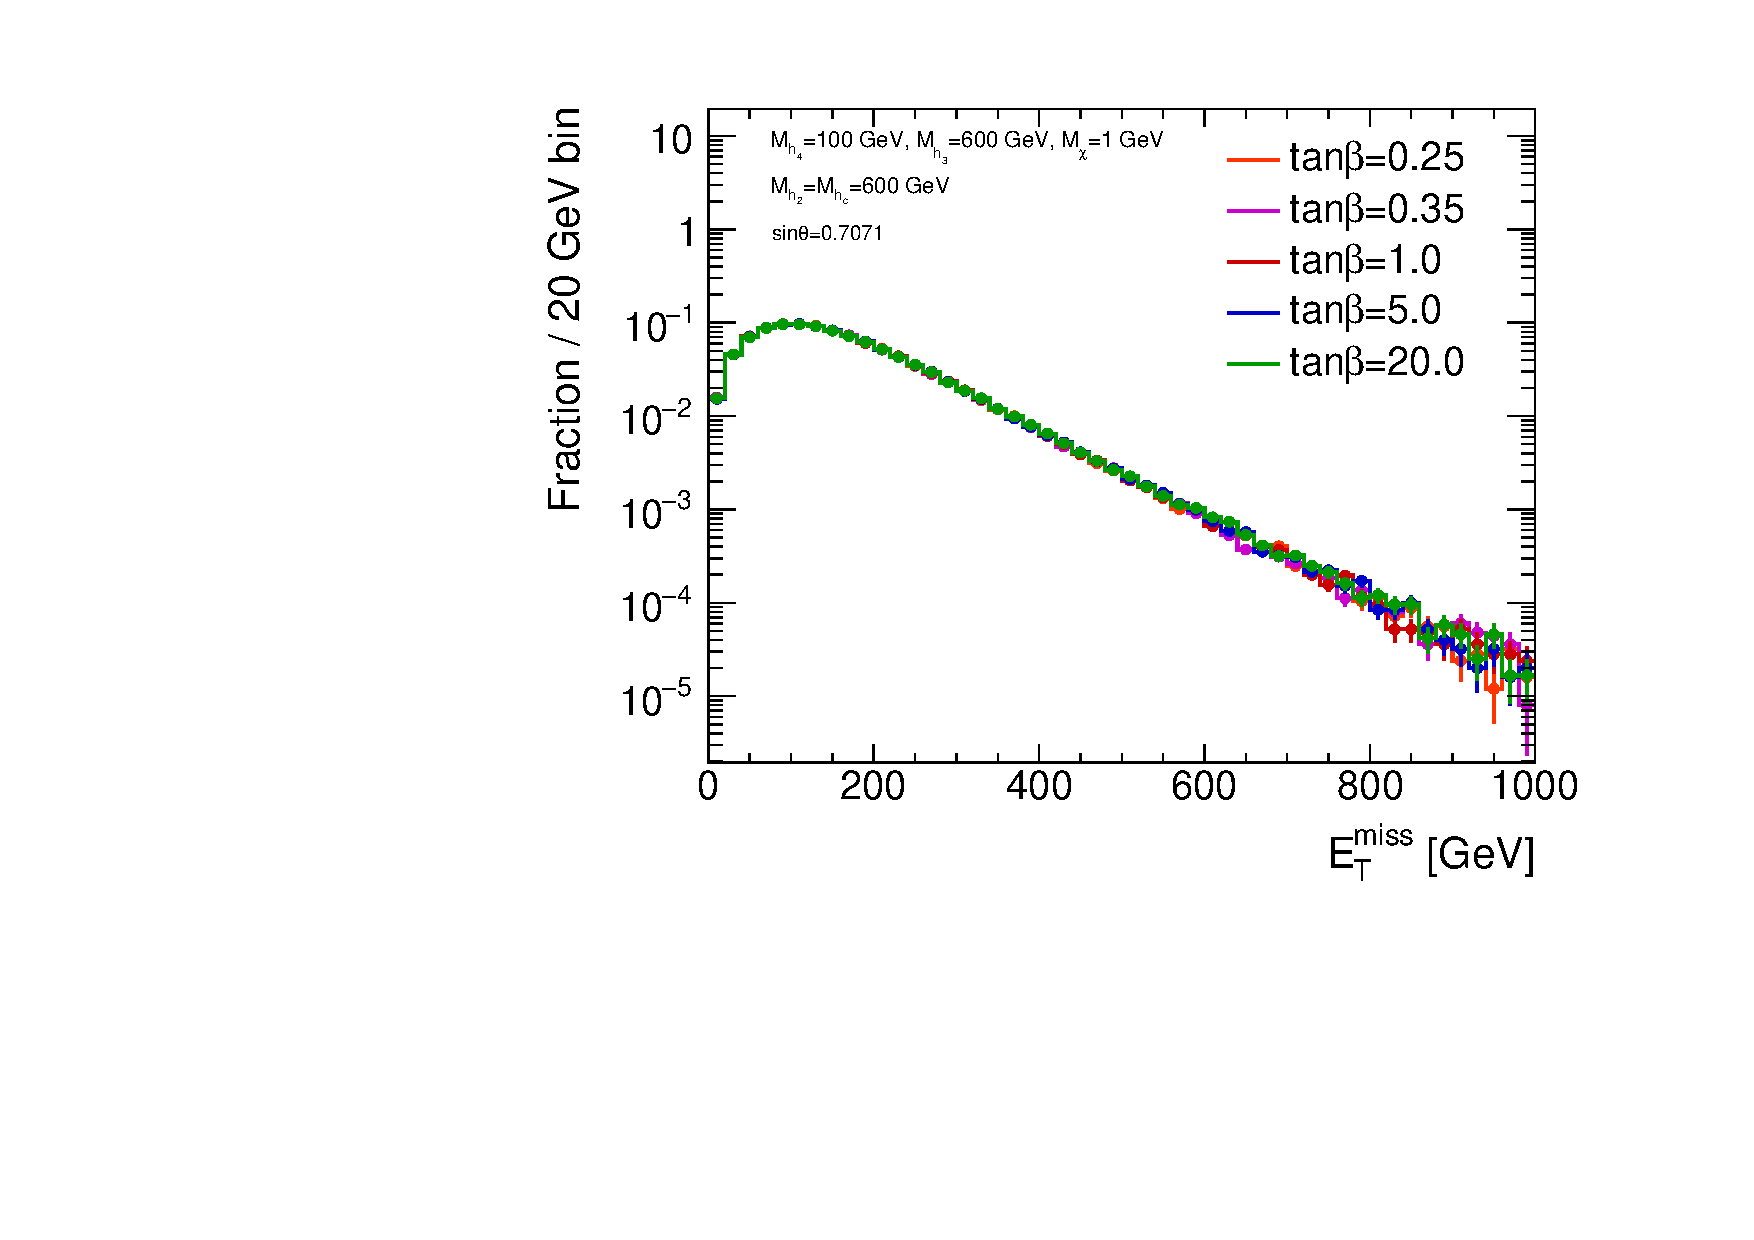
\includegraphics[width=\textwidth]{texinputs/04_grid/figures/DMHF/benchmarking/MDM_1_Ma_100_MA_600_sinp_0.7071_SCAN_tanb_decayed/metlog.pdf}
    \caption{$E_{T}^{miss}$}
  \end{subfigure}
  \begin{subfigure}[b]{0.49\textwidth}
    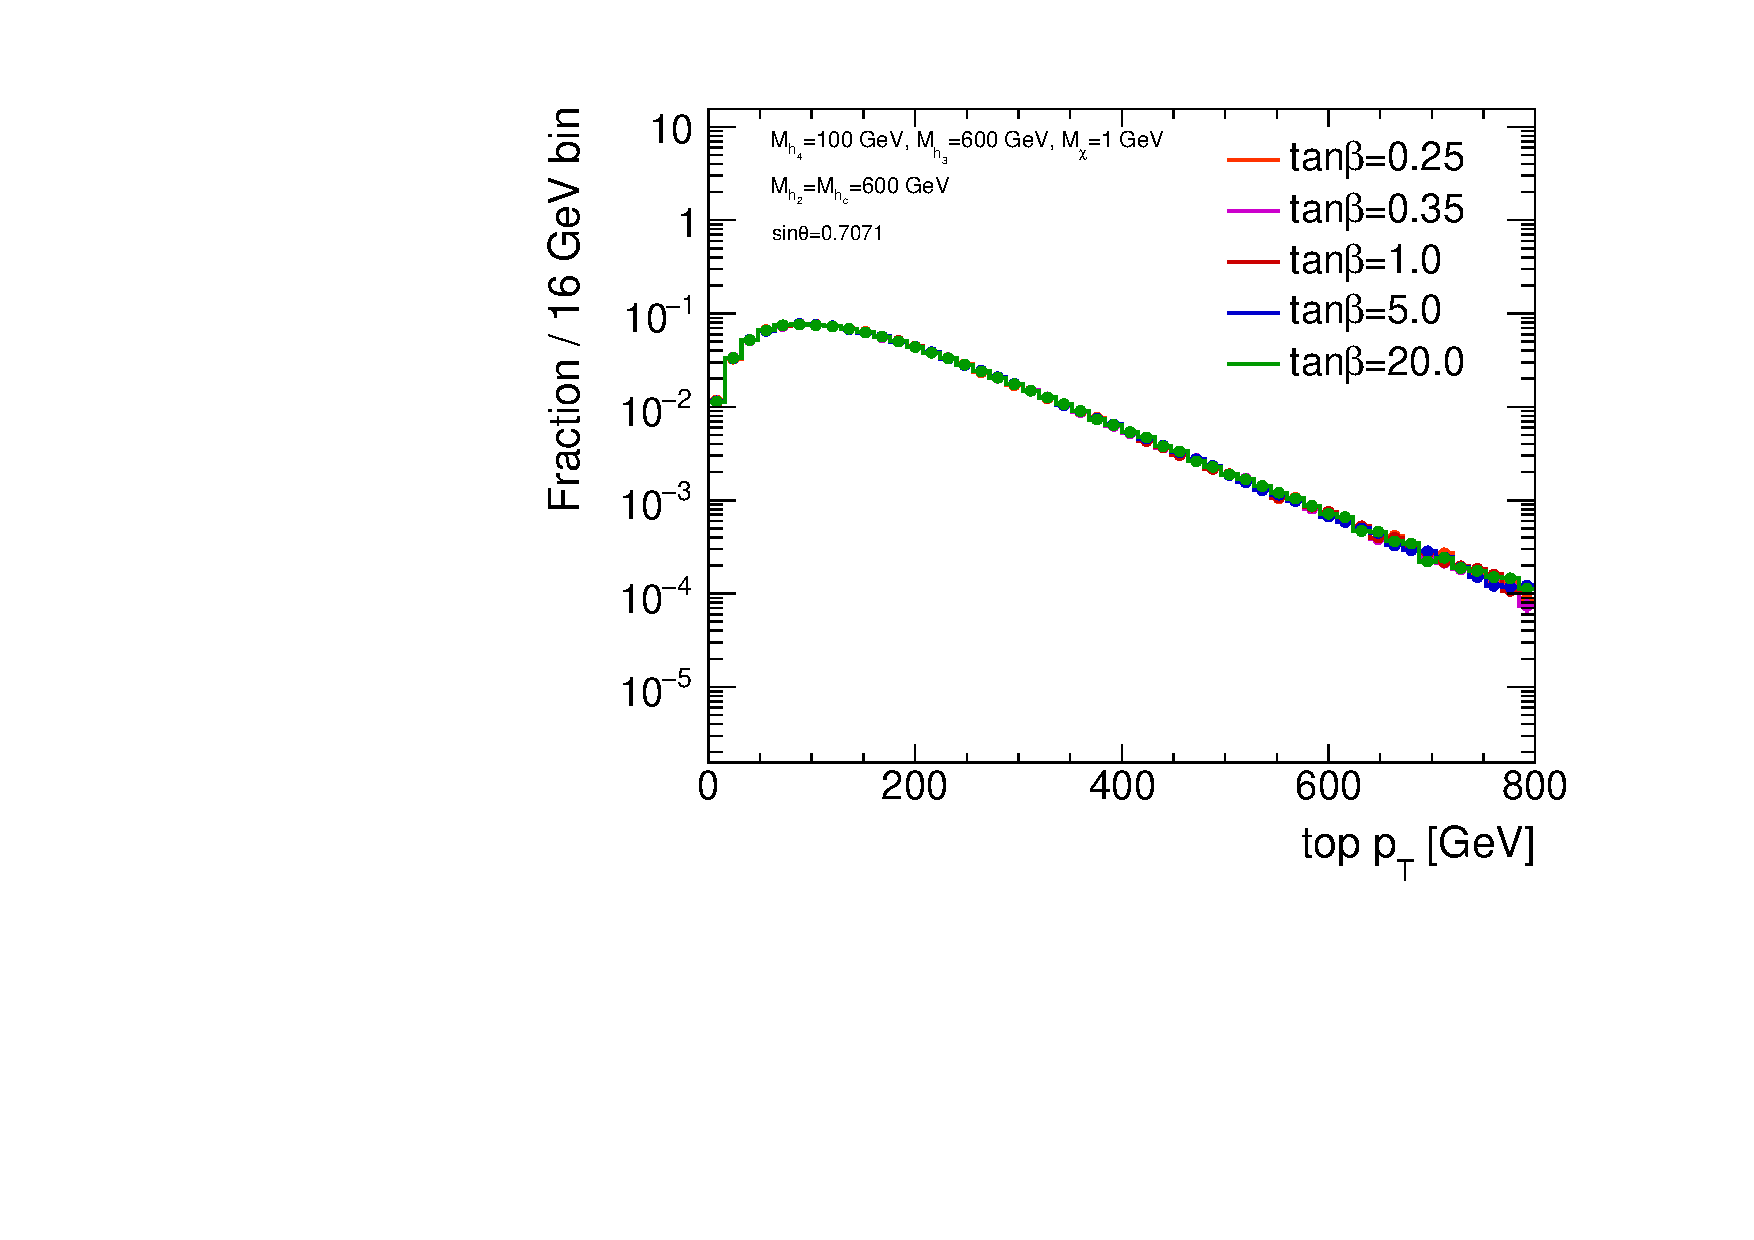
\includegraphics[width=\textwidth]{texinputs/04_grid/figures/DMHF/benchmarking/MDM_1_Ma_100_MA_600_sinp_0.7071_SCAN_tanb_decayed/topptlog.pdf}
    \caption{top $p_{T}$}
  \end{subfigure}
  \caption{The $E_{T}^{miss}$ and top $p_{T}$ distribution for inclusive $t\bar{t}+\chi\bar{\chi}$ production for various values of $\tan\beta$, with $\mathrm{M_a}=100$ GeV, $\mathrm{M_A}=600$ GeV, $\mathrm{M_H}=\mathrm{M_{H^{\pm}}}=6
00$ GeV, and $\sin\theta=0.7071$.}
  \label{fig:kin_tanB}
\end{figure}

\begin{figure}
  \centering
  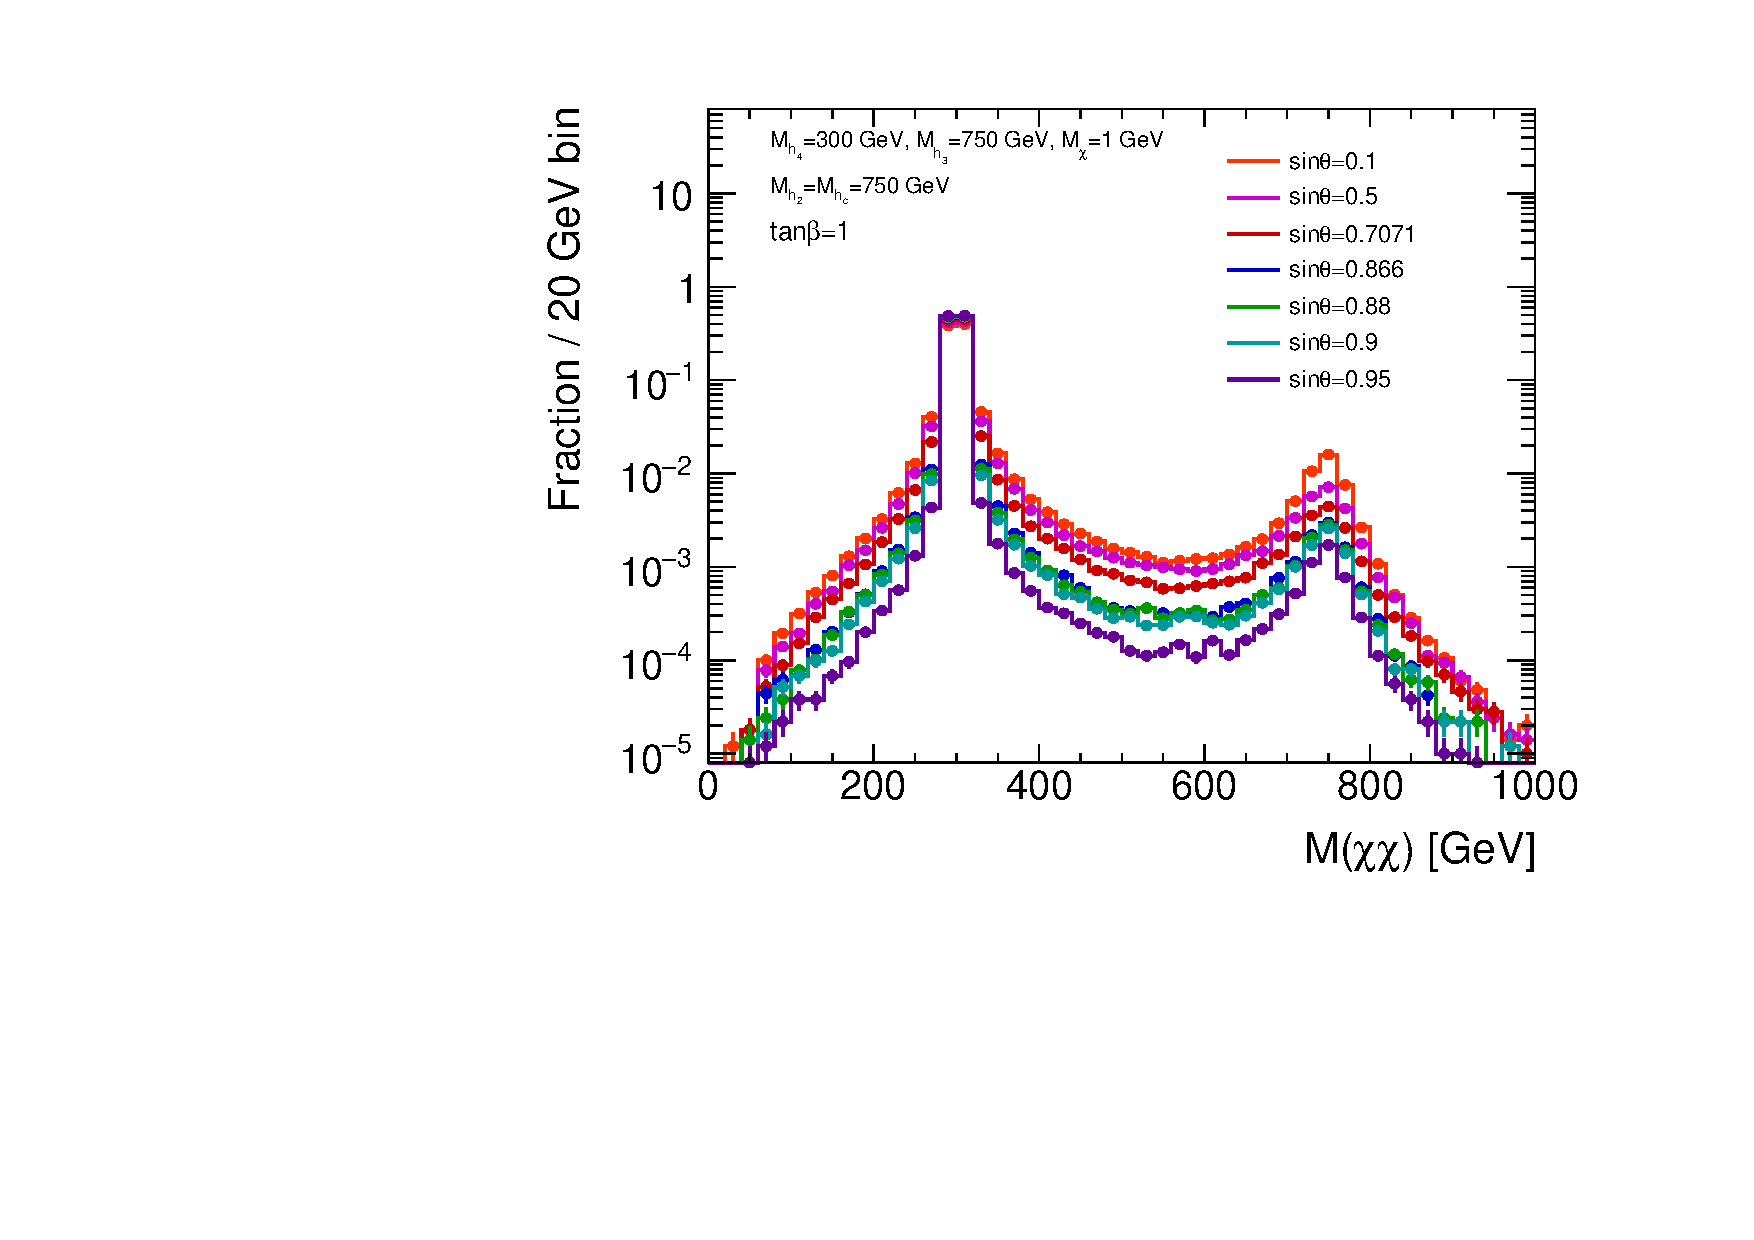
\includegraphics[width=0.6\textwidth]{texinputs/04_grid/figures/DMHF/benchmarking/MDM_1_Ma_300_MA_750_tanb_1.0_SCAN_sinp_v2/mchichi.pdf}
  \caption{The mass distribution of the $\chi \bar{\chi}$ system for various values of $\sin\theta$, with $\mathrm{M_a}=300$ GeV, $\mathrm{M_A}=750$ GeV, $\mathrm{M_H}=\mathrm{M_{H^{\pm}}}=750$ GeV, and $\tan\beta=1$.}
  \label{fig:mchichi_sinp}
\end{figure} 

\begin{figure}
  \centering
  \begin{subfigure}[b]{0.49\textwidth}
    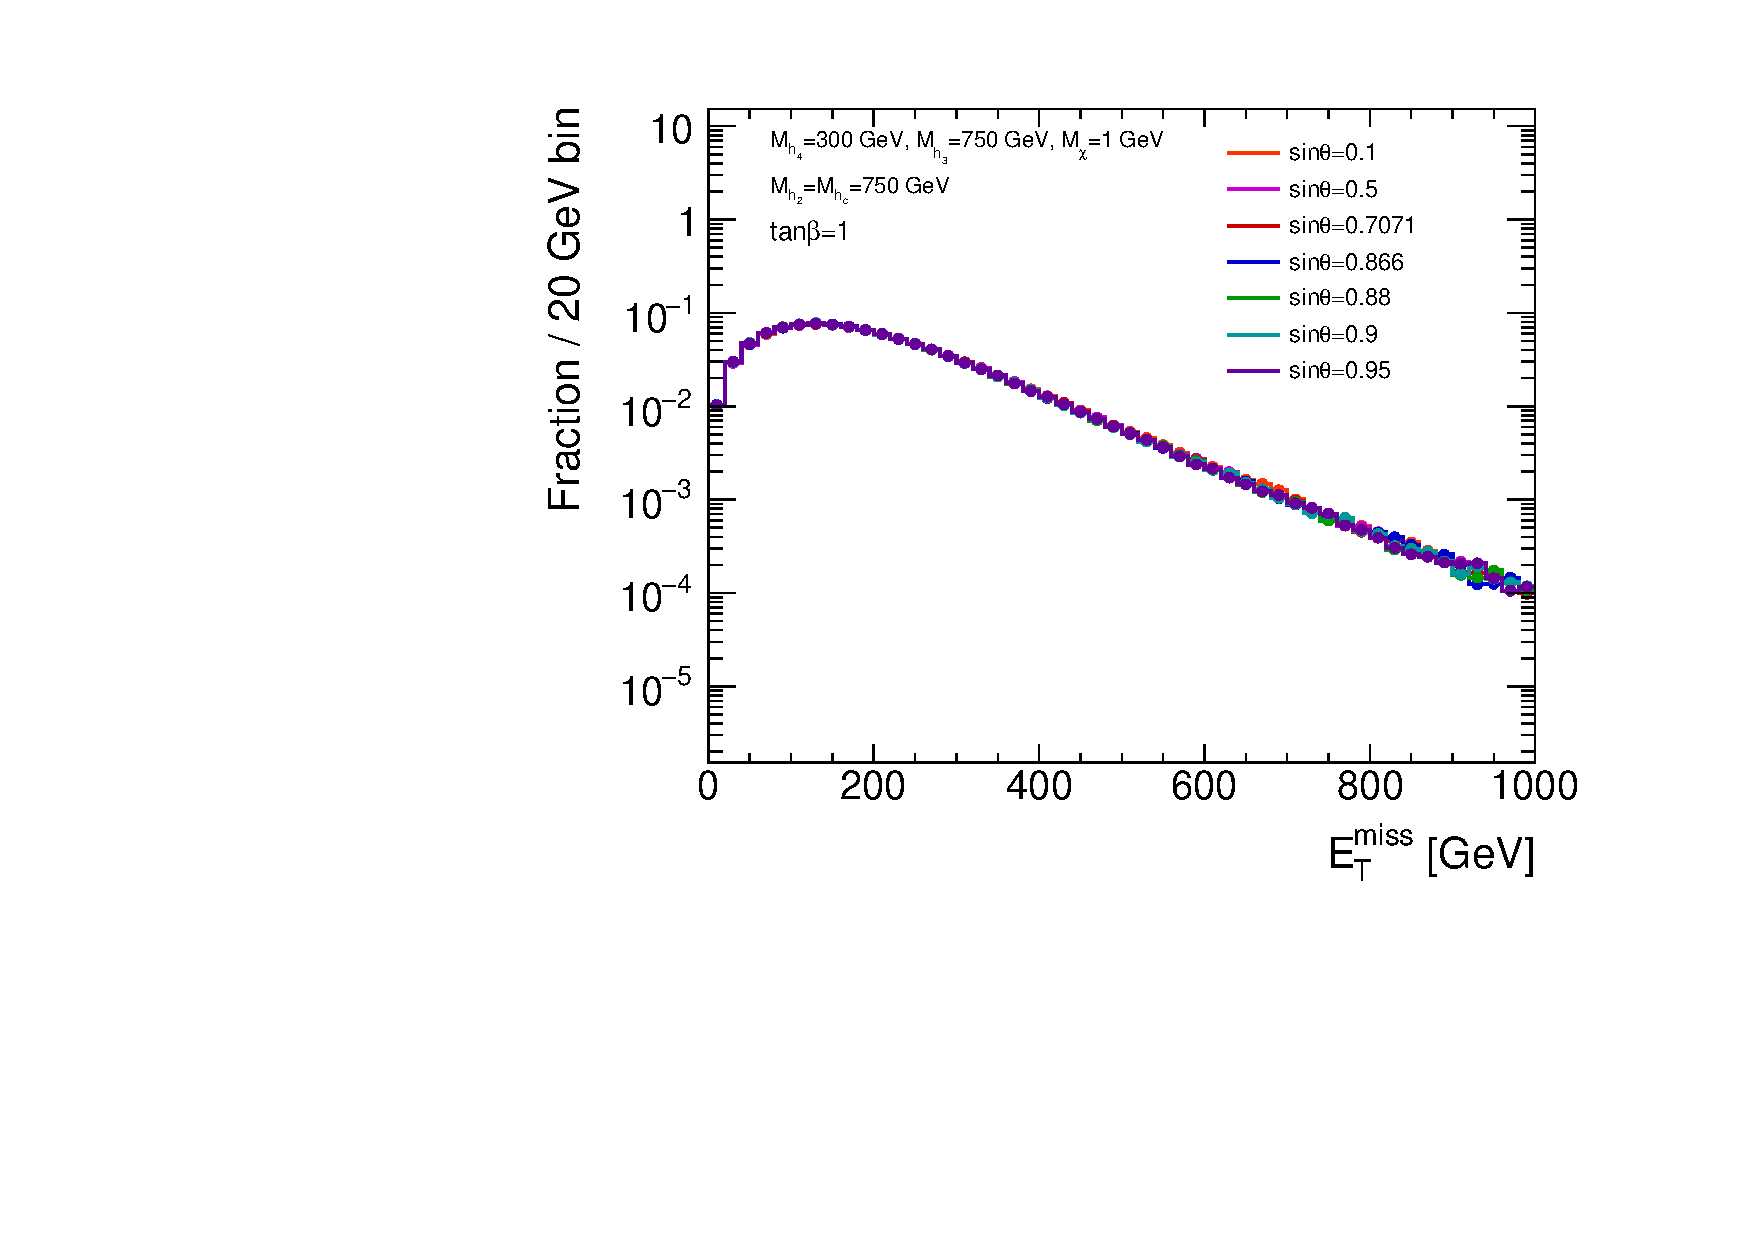
\includegraphics[width=\textwidth]{texinputs/04_grid/figures/DMHF/benchmarking/MDM_1_Ma_300_MA_750_tanb_1.0_SCAN_sinp_v2/metlog.pdf}
    \caption{$E_{T}^{miss}$}
  \end{subfigure}
  \begin{subfigure}[b]{0.49\textwidth}
    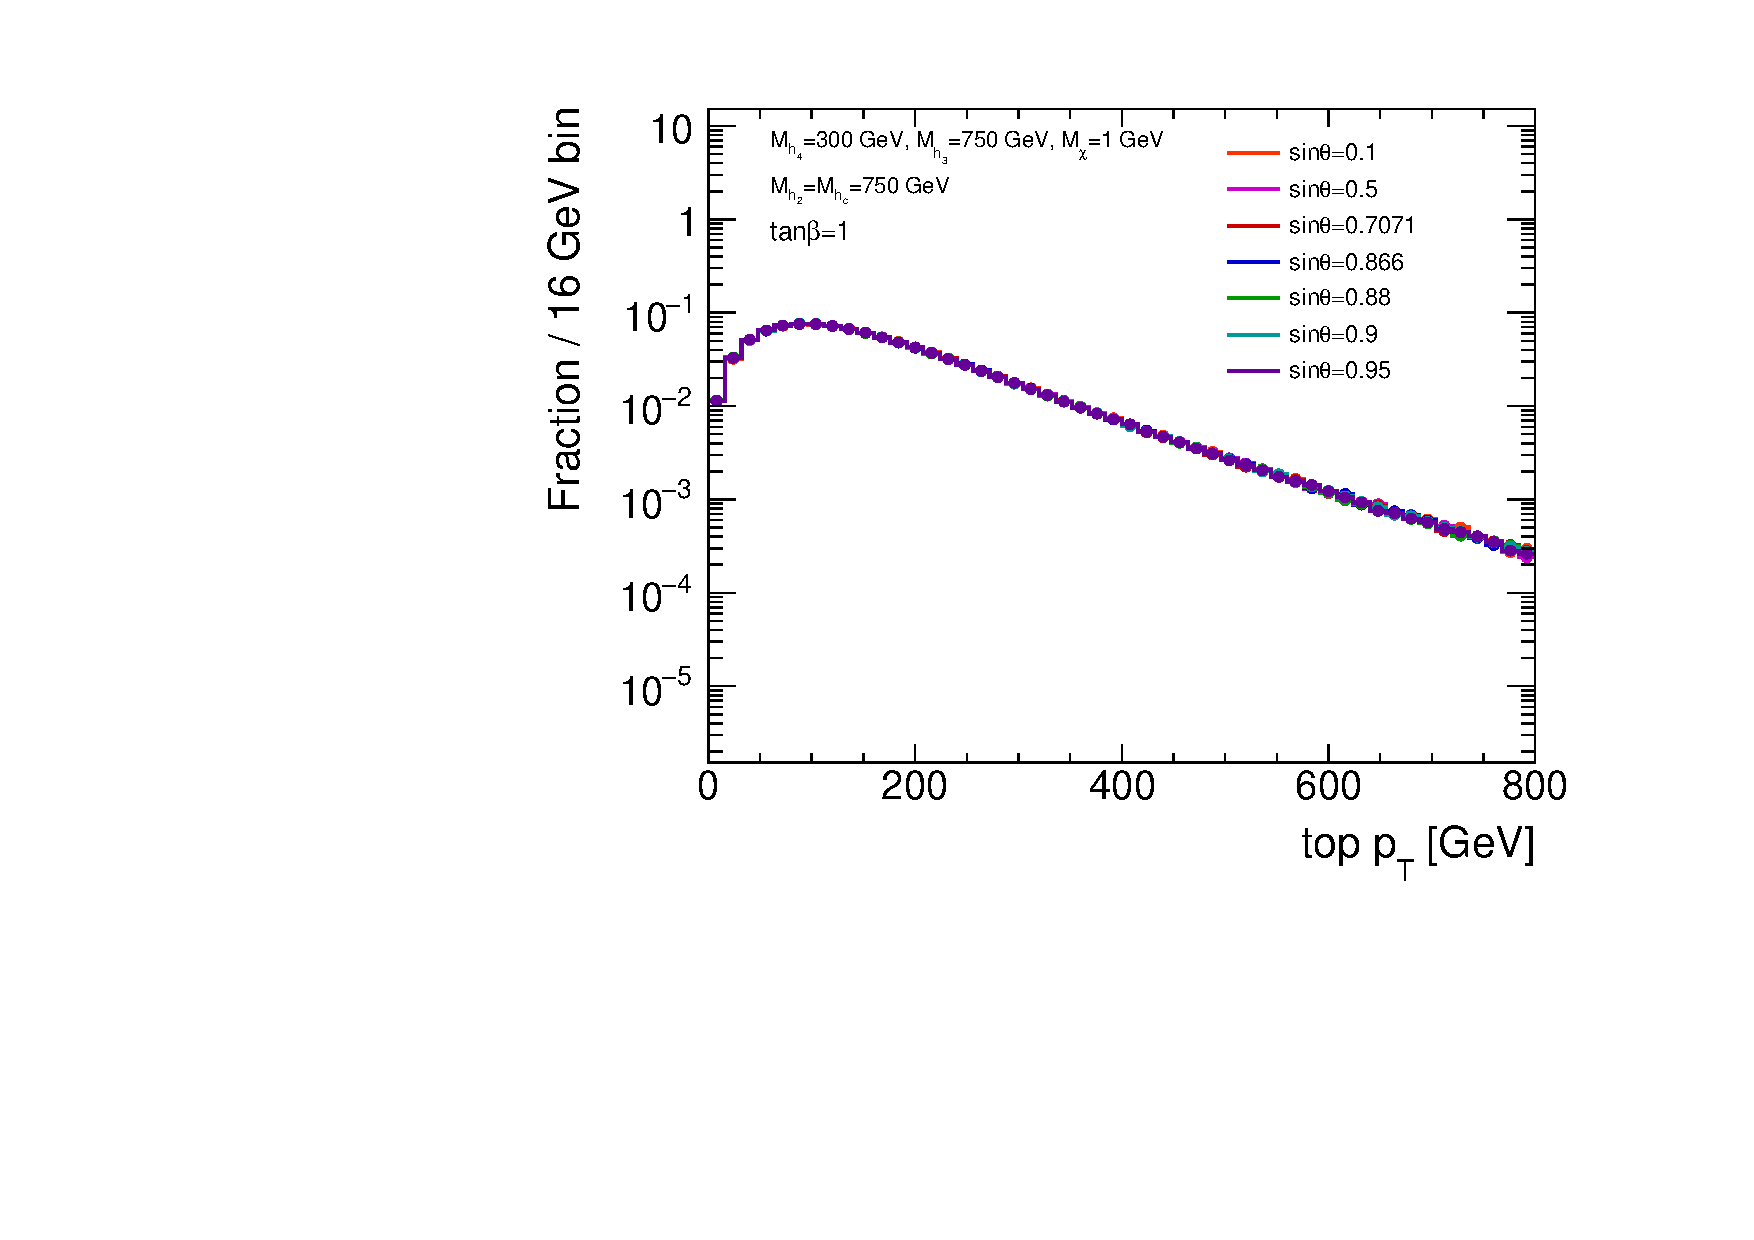
\includegraphics[width=\textwidth]{texinputs/04_grid/figures/DMHF/benchmarking/MDM_1_Ma_300_MA_750_tanb_1.0_SCAN_sinp_v2/topptlog.pdf}
    \caption{top $p_{T}$}
  \end{subfigure}
  \caption{The $E_{T}^{miss}$ and top $p_{T}$ distribution for inclusive $t\bar{t}+\chi\bar{\chi}$ production for various values of $\sin\theta$, with $\mathrm{M_a}=300$ GeV, $\mathrm{M_A}=750$ GeV, $\mathrm{M_H}=\mathrm{M_{H^{\pm}}}=750$ GeV, and $\tan\beta=1$.}
  \label{fig:kin_sinp}
\end{figure}

In the limit of small $\tan\beta$ values, the couplings of $h_{3}$ (A) and $h_{4}$ (a) to down-type quarks are heavily suppressed irrespectively of the Yukawa assignment. At LO, $t\bar{t}+\chi\bar{\chi}$ associated production is mediated through either CP-odd weak eigenstate, A or a, though it is shown in Fig.~\ref{fig:mchichi_tanB} that $a\rightarrow\chi\bar{\chi}$ is the dominant production mode. Although the relative medatior contribution is dependent on $\tan\beta$, observables such as $E_{T}^{miss}$ and top quark $p_{T}$ do not have a kinematic dependence on $\tan\beta$ as demonstrated in Fig.~\ref{fig:kin_tanB}.

Mixing of the CP-odd weak eigenstates is achieved through the mixing angle, $\theta$. As shown in Fig.~\ref{fig:mchichi_sinp}, the A and a mass peaks are quite narrow for values where $\sin\theta$ approaches 1, and $a\rightarrow\chi\bar{\chi}$ is the dominant $\chi\bar{\chi}$ production mode. However, no kinematic dependence on $\sin\theta$ is observed in the $E_{T}^{miss}$ and top quark $p_{T}$ as shown in Fig.~\ref{fig:kin_sinp}.

\paragraph{Scan of $\mathrm{M_{a}}$ and $\mathrm{M_{A}}$:}

While the relevant kinematic distributions display no dependence on the aforementioned mixing angles, the same does not hold true for the masses, $\mathrm{M_{a}}$ and $\mathrm{M_{A}}$. As shown in Fig.~\ref{fig:kin_Ma}, the $E_{T}^{miss}$, and leading and trailing top quark $p_{T}$ distributions broaden with increasing $\mathrm{M_{a}}$. Similarly, for values of $\mathrm{M_{A}} < \mathrm{M_{a}}$, as $\mathrm{M_{A}}$ increases, the kinematic distributions mentioned above also broaden, as shown in Fig.~\ref{fig:kin_MA}.

\begin{figure}
  \centering
  \begin{subfigure}[b]{0.49\textwidth}
    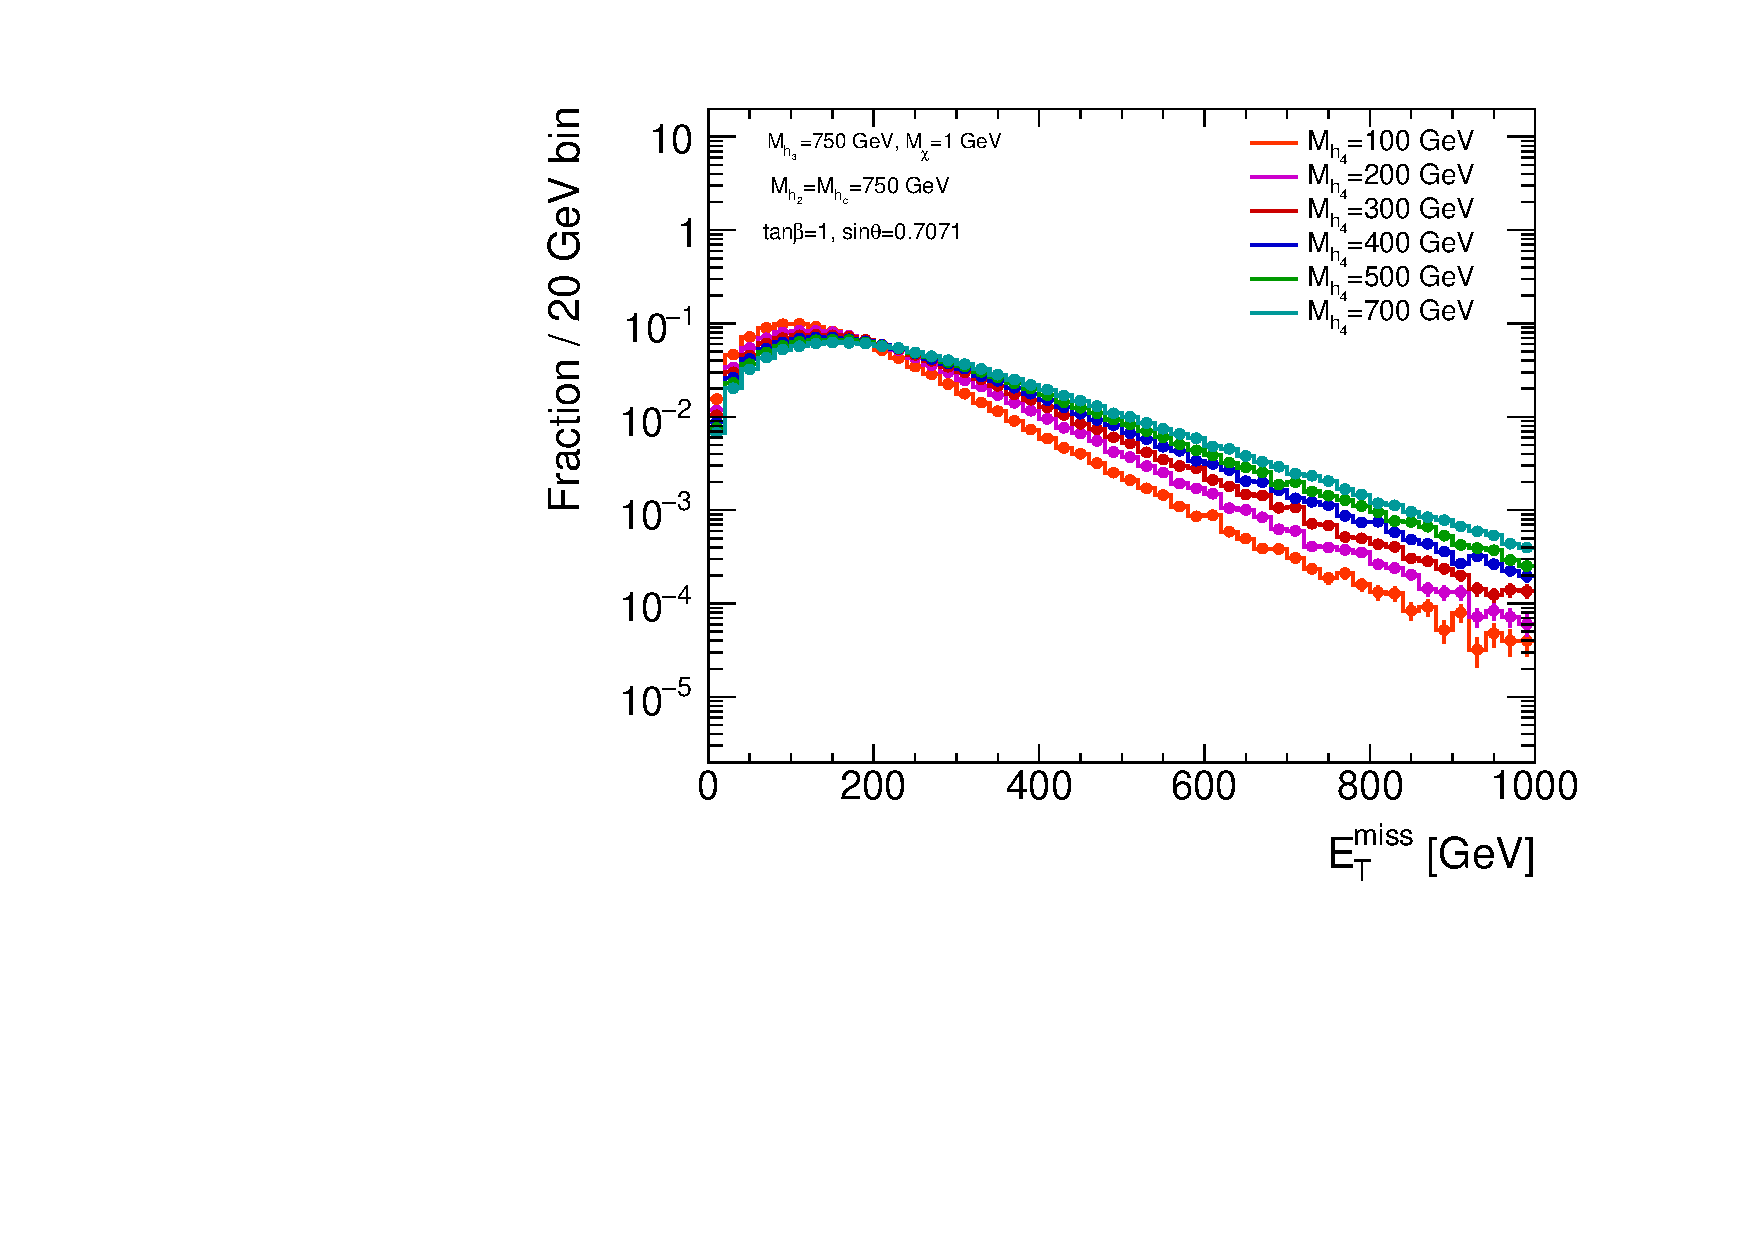
\includegraphics[width=\textwidth]{texinputs/04_grid/figures/DMHF/benchmarking/MDM_1_MA_750_sinp_0.7071_tanb_1.0_SCAN_Ma/metlog.pdf}
    \caption{$E_{T}^{miss}$}
  \end{subfigure}
  \begin{subfigure}[b]{0.49\textwidth}
    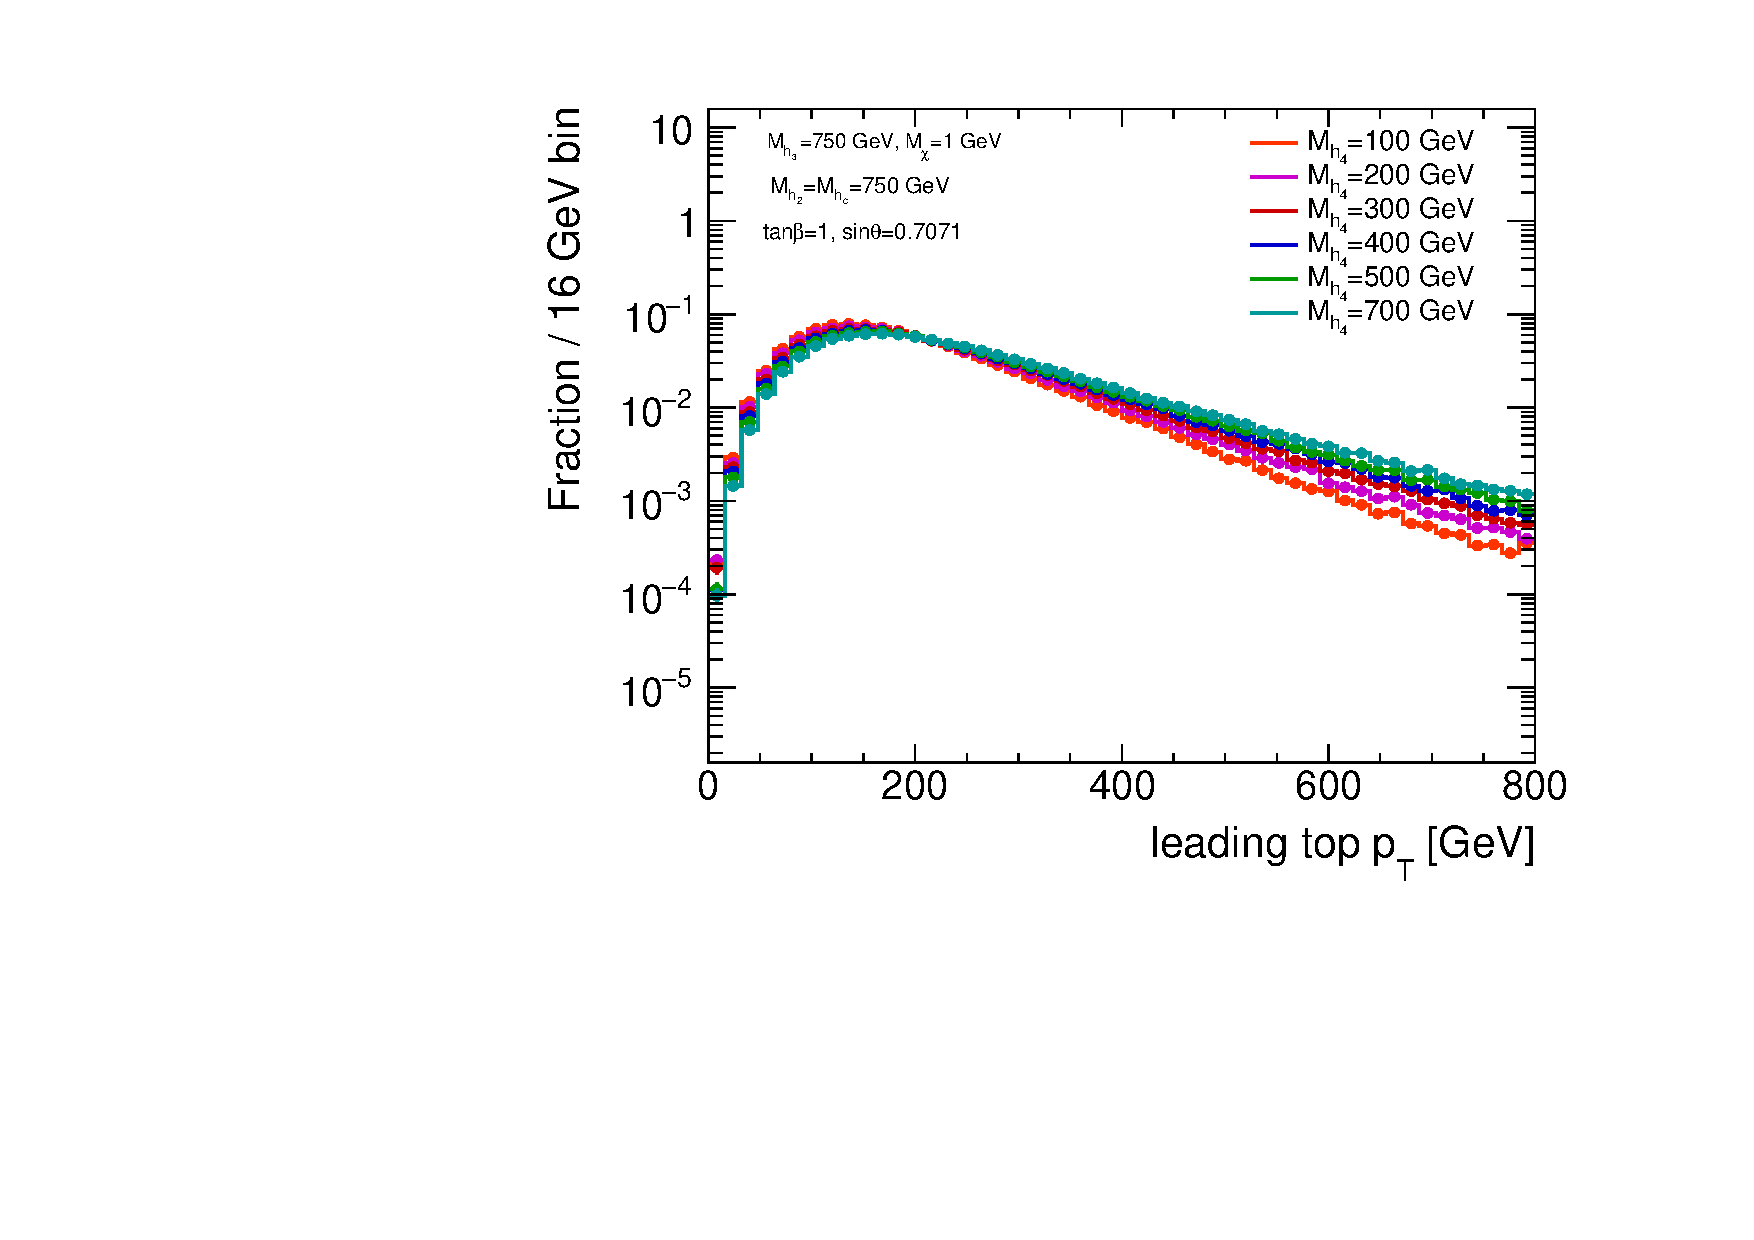
\includegraphics[width=\textwidth]{texinputs/04_grid/figures/DMHF/benchmarking/MDM_1_MA_750_sinp_0.7071_tanb_1.0_SCAN_Ma/top1ptlog.pdf}
    \caption{Leading top $p_{T}$}
  \end{subfigure} \\
  \begin{subfigure}[b]{0.49\textwidth}
    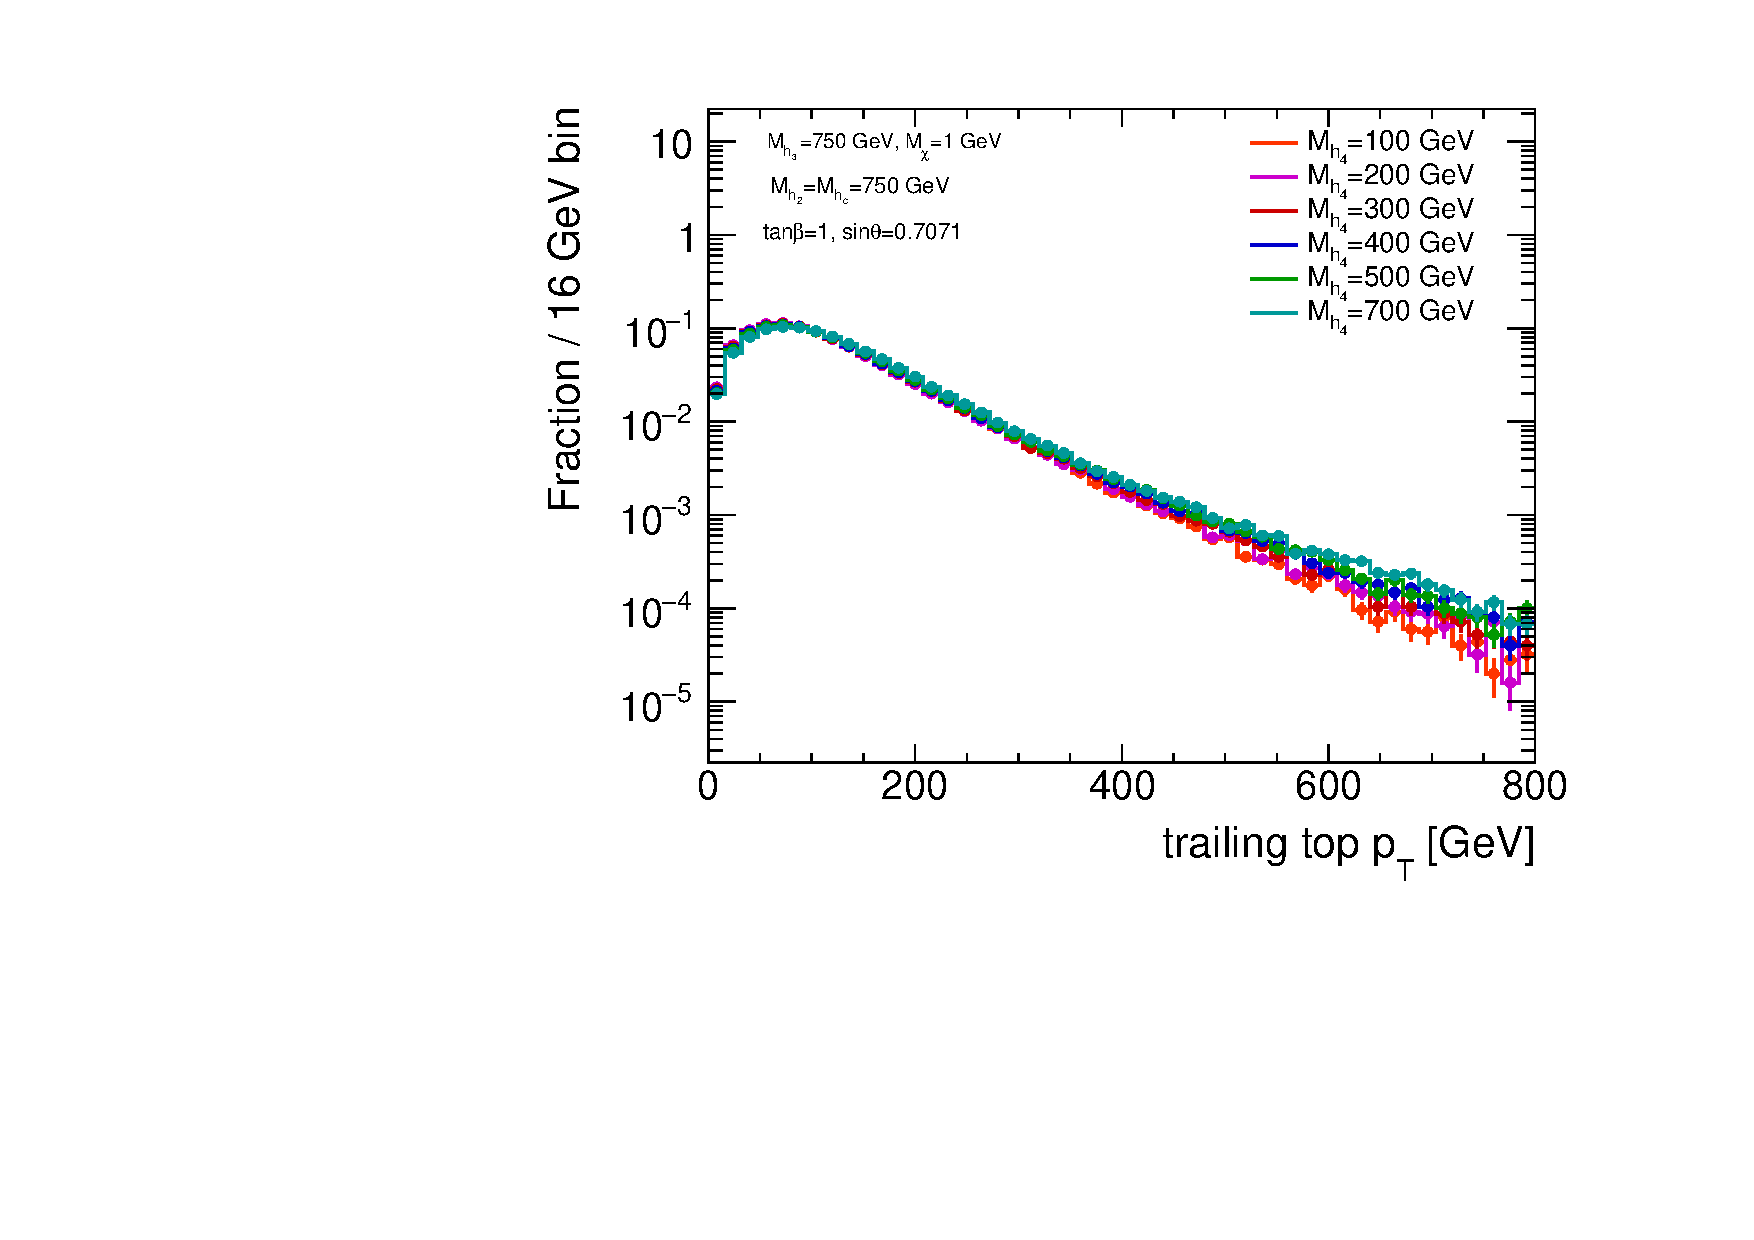
\includegraphics[width=\textwidth]{texinputs/04_grid/figures/DMHF/benchmarking/MDM_1_MA_750_sinp_0.7071_tanb_1.0_SCAN_Ma/top2ptlog.pdf}
    \caption{Trailing top $p_{T}$}
  \end{subfigure}
  \caption{The $E_{T}^{miss}$, leading and trailing top $p_{T}$ distributions for inclusive $t\bar{t}+\chi\bar{\chi}$ production for various values of $\mathrm{M_a}$, with $\mathrm{M_A}=750$ GeV, $\mathrm{M_H}=\mathrm{M_{H^{\pm}}}=750$ GeV, $\tan\beta=1$, and $\sin\theta=0.7071$.}
  \label{fig:kin_Ma}
\end{figure}

\begin{figure}
  \centering
  \begin{subfigure}[b]{0.49\textwidth}
    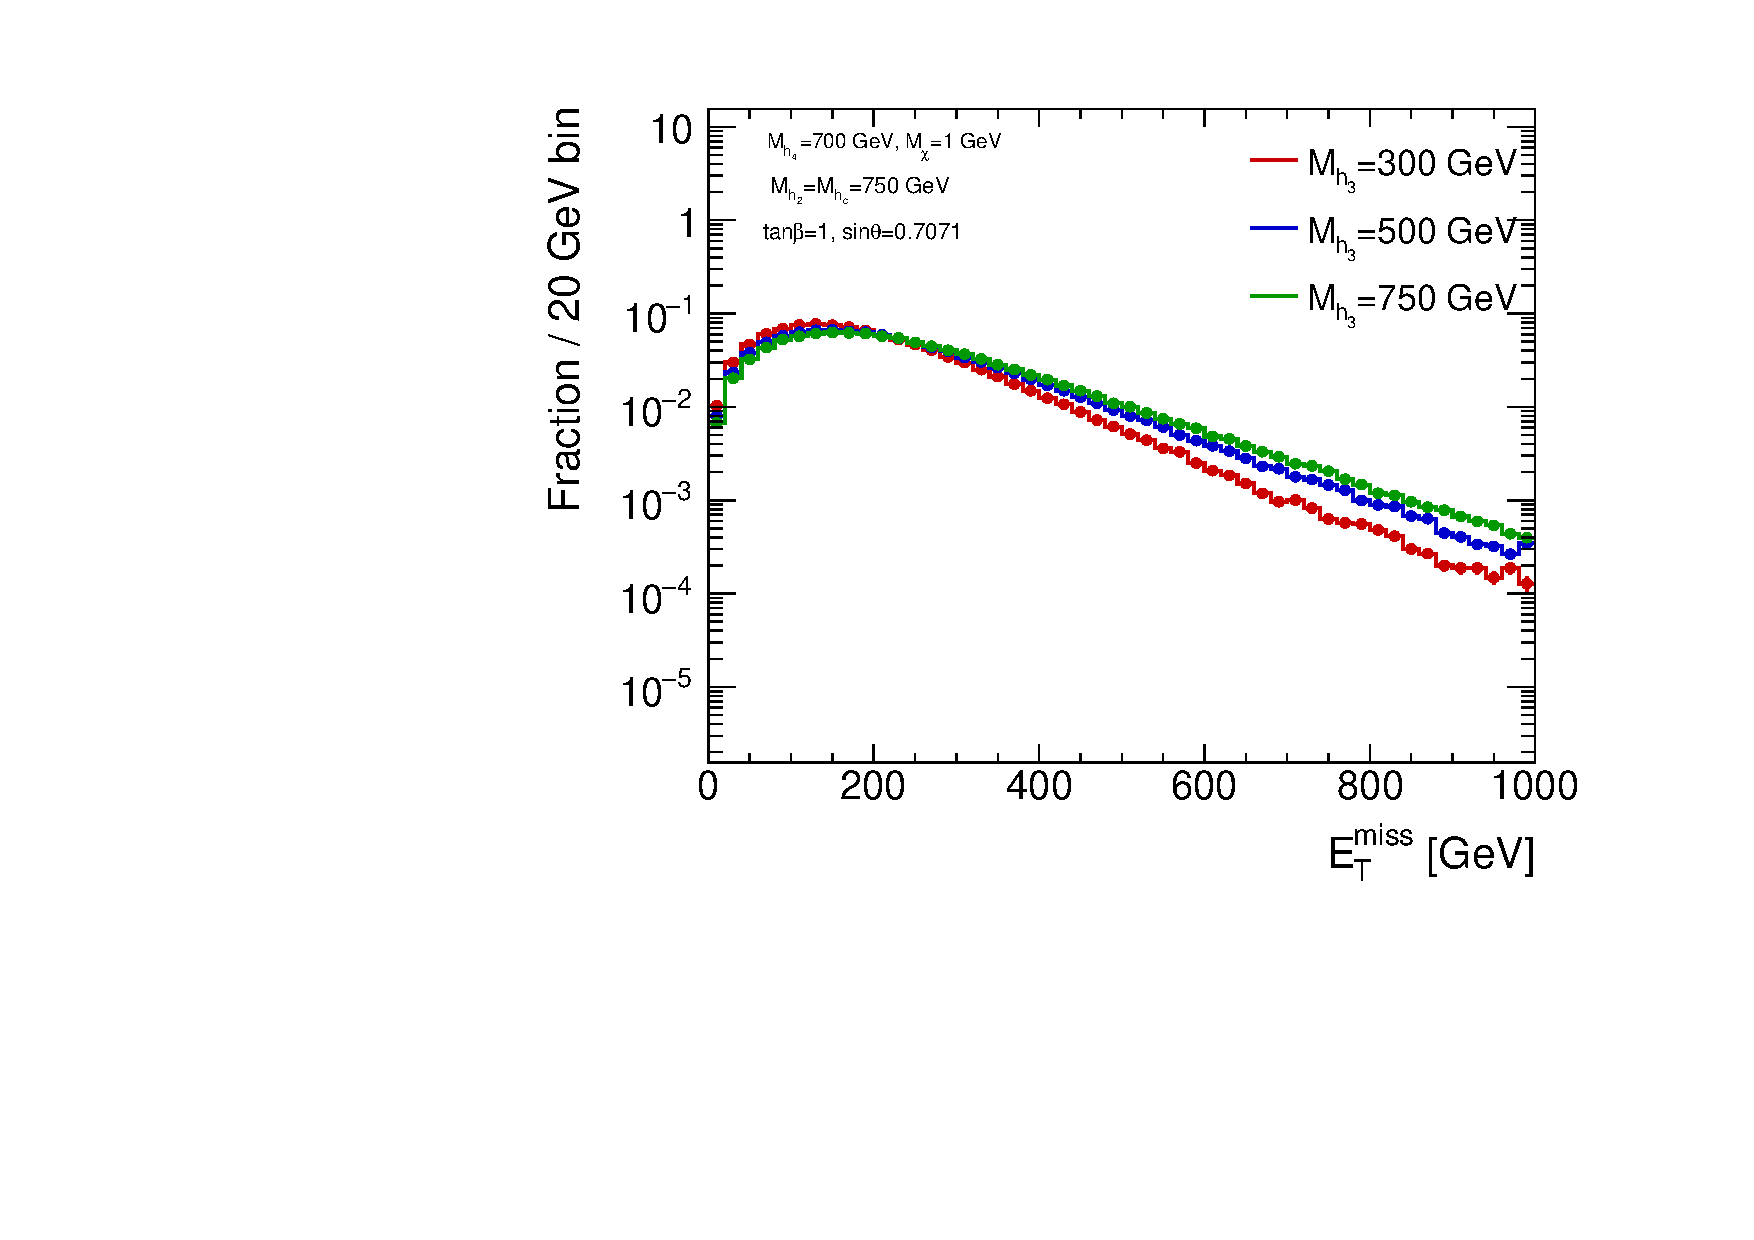
\includegraphics[width=\textwidth]{texinputs/04_grid/figures/DMHF/benchmarking/MDM_1_Ma_700_sinp_0.7071_tanb_1.0_SCAN_MA/metlog.pdf}
    \caption{$E_{T}^{miss}$}
  \end{subfigure}
  \begin{subfigure}[b]{0.49\textwidth}
    \includegraphics[width=\textwidth]{texinputs/04_grid/figures/DMHF/benchmarking/MDM_1_Ma_700_sinp_0.7071_tanb_1.0_SCAN_MA/top1ptlog.pdf}
    \caption{Leading top $p_{T}$}
  \end{subfigure} \\
  \begin{subfigure}[b]{0.49\textwidth}
    \includegraphics[width=\textwidth]{texinputs/04_grid/figures/DMHF/benchmarking/MDM_1_Ma_700_sinp_0.7071_tanb_1.0_SCAN_MA/top2ptlog.pdf}
    \caption{Trailing top $p_{T}$}
  \end{subfigure}
  \caption{The $E_{T}^{miss}$, leading and trailing top $p_{T}$ distributions for inclusive $t\bar{t}+\chi\bar{\chi}$ production for various values of $\mathrm{M_A}$, with $\mathrm{M_a}=700$ GeV, $\mathrm{M_H}=\mathrm{M_{H^{\pm}}}=750$ GeV, $\tan\beta=1$, and $\sin\theta=0.7071$.}
  \label{fig:kin_MA}
\end{figure}
%%%%-----------------------------------------------------------------------------------------
\subsubsection{Comparison with DMsimp Pseudoscalar Model}

To date, simplified models of DM (\texttt{DMsimp}) are used to interpret Run II CMS and ATLAS HF+DM searches. A comparison of the pertinent kinematic distributions between the pseudoscalar simplified model and the 2HDM+a model for the same value of $\mathrm{M_{a}}$ are shown in Fig.~\ref{kin_DMSimpV2HDMa}. The kinematics of the pseudoscalar \texttt{DMsimp} model with $\mathrm{M_{a}}=100$ GeV map directly onto those of the 2HDM+a model with $\mathrm{M_{a}}=100$ GeV, $\mathrm{M_{A}}=600$ GeV, $\mathrm{M_{H}}=\mathrm{M_{H^{\pm}}}=600$ GeV, $\sin\theta=0.7071$, and $\tan\beta=1$. From the mass distribution of the $\chi\bar{\chi}$ shown in Fig.~\ref{fig:mchichi_DMsimpV2HDMa}, it is evident that the 2HDM+a model contains contributions from both the light and heavy pseudoscalar mediator as in the \texttt{DMsimp} model.

\begin{figure}
  \centering
  \begin{subfigure}[b]{0.49\textwidth}
    \includegraphics[width=\textwidth]{texinputs/04_grid/figures/DMHF/benchmarking/MDM_1_Ma_100_MA_600_sinp_0.7071_tanb_1.0_VS_DMSimp_100_600_Decayed/metlog.pdf}
    \caption{$E_{T}^{miss}$}
  \end{subfigure}
  \begin{subfigure}[b]{0.49\textwidth}
    \includegraphics[width=\textwidth]{texinputs/04_grid/figures/DMHF/benchmarking/MDM_1_Ma_100_MA_600_sinp_0.7071_tanb_1.0_VS_DMSimp_100_600_Decayed/top1ptlog.pdf}
    \caption{Leading top $p_{T}$}
  \end{subfigure} \\
  \begin{subfigure}[b]{0.49\textwidth}
    \includegraphics[width=\textwidth]{texinputs/04_grid/figures/DMHF/benchmarking/MDM_1_Ma_100_MA_600_sinp_0.7071_tanb_1.0_VS_DMSimp_100_600_Decayed/top2ptlog.pdf}
    \caption{Trailing top $p_{T}$}
  \end{subfigure}
  \caption{The $E_{T}^{miss}$, leading and trailing top $p_{T}$ distributions for inclusive $t\bar{t}+\chi\bar{\chi}$ production for various values of $\mathrm{M_A}$, with $\mathrm{M_a}=700$ GeV, $\mathrm{M_H}=\mathrm{M_{H^{\pm}}}=750$ GeV, $\tan\beta=1$, and $\sin\theta=0.7071$.}
  \label{fig:kin_DMSimpV2HDMa}
\end{figure}

\begin{figure}
  \centering
  \includegraphics[width=0.6\textwidth]{texinputs/04_grid/figures/DMHF/benchmarking/MDM_1_Ma_100_MA_600_sinp_0.7071_tanb_1.0_VS_DMSimp_100_600_Decayed/mchichi.pdf}
  \caption{The mass distribution of the $\chi\bar{\chi}$ system for \texttt{DMsimp} pseudoscalar models with $\mathrm{M_a}=100$ GeV and $\mathrm{M_a}=600$ GeV, compared with 2HDM+a with $\mathrm{M_a}=100$ GeV, $\mathrm{M_A}=600$ GeV, $\mathrm{M_H}=\mathrm{M_{H^{\pm}}}=600$ GeV, $\sin\theta=0.7071$ and $\tan\beta=1$.}
  \label{fig:mchichi_DMsimpV2HDMa}
\end{figure}

In Fig.~\ref{fig:DMSimpV2HDMa}, relevant kinematic distributions, commonly employed in HF+DM searches, are mapped from the \texttt{DMsimp} pseudoscalar models to the 2HDM+a model, with the mediator masses corresponding to the additional light pseudoscalar in the latter model. The dashed distributions represent the \texttt{DMsimp} model, while the solid are the 2HDM+a model distributions. The $t\bar{t}+\chi\bar{\chi}$ process was generated at LO precision using both models. As can be seen, the kinematics do not change appreciably between the models generated at the same value of $\mathrm{M_{a}}$. A discussion on cross-section rescaling procedures can be found in the following section.

\begin{figure}
  \centering    
  \begin{subfigure}[b]{0.49\textwidth}
    \includegraphics[width=\textwidth]{texinputs/04_grid/figures/DMHF/benchmarking/MDM_1_MA_600_sinp_0.7071_tanb_1.0_DMsimpV2HDMa/metlog.pdf}
    \caption{$E_{T}^{miss}$}
  \end{subfigure}
  \begin{subfigure}[b]{0.49\textwidth}
    \includegraphics[width=\textwidth]{texinputs/04_grid/figures/DMHF/benchmarking/MDM_1_MA_600_sinp_0.7071_tanb_1.0_DMsimpV2HDMa/top1ptlog.pdf}
    \caption{Leading top $p_{T}$}
  \end{subfigure} \\
  \begin{subfigure}[b]{0.49\textwidth}
    \includegraphics[width=\textwidth]{texinputs/04_grid/figures/DMHF/benchmarking/MDM_1_MA_600_sinp_0.7071_tanb_1.0_DMsimpV2HDMa/top2ptlog.pdf}
    \caption{Trailing top $p_{T}$}
  \end{subfigure}
  \caption{The $E_{T}^{miss}$, leading and trailing top $p_{T}$ distributions for inclusive $t\bar{t}+\chi\bar{\chi}$ production generated from the \texttt{DMsimp} (solid) and the 2HDM+a (dashed) models with various values of $\mathrm{M_a}$. The 2HDM+a models are generated with the following model parameters:$\mathrm{M_A}=600$ GeV, $\mathrm{M_H}=\mathrm{M_{H^{\pm}}}=600$ GeV, $\tan\beta=1$, and $\sin\theta=0.7071$.}
\label{fig:DMSimpV2HDMa}
\end{figure}
%%%%-----------------------------------------------------------------------------------------
\subsubsection{Recasting existing tt+\met and bb+\met signatures}
\label{subsub:hfttrecast}
These two signatures are dominantly produced in diagrams involving the invisible decays of the two CP-odd scalars. 
Their relevance is therefore determined by the two pseudoscalar masses, $m(A)$ and $m(a)$ and it is a function of 
$sin\theta$ and $tan\beta$. 
For both $bb$ and $tt$ associated productions, we find that the
highest sensitivity of this signatures is obtained for high values of $sin\theta$.

The 2HDM+a model is equivalent to a single pseudoscalar simplified
model (DMF) when $A$ is much heavier than $a$, and therefore the
former does not contribute to the considered final state. However,
when the two mediators are closer in mass, the $pp\rightarrow ttA$
contribution becomes more relevant  as it is possible to observe in 
Figure~\ref{fig:mdd}, where the two models are compared
assuming $m(A) = 750$ GeV and two different values
for $m(a)$. An excellent agreement was observed between
$DMSIMP$ and $2HDMp$ on parton-level variables sensitive 
to the helicity structure of the interaction between top and the
mediator\cite{Haisch:2016gry}, if the invariant mass of the two DM
particles in the 2HDM is required to be smalle than 200(300)~GeV for
$m(a)=150(300)$~GeV respectively, giving confidence that,
once the contribution from $A$ production is separated, it is possible
to fully map the $2HDM+a$ kinematics into the DMF simplified model. 


\begin{figure}[htb]
\begin{center}
\includegraphics[width=0.48\textwidth]{texinputs/04_grid/figures/DMHF/mdd150.pdf}
\includegraphics[width=0.48\textwidth]{texinputs/04_grid/figures/DMHF/mdd300.pdf}
\caption{Comparison of $m(\chi\chi)$, the invariant mass of 
the two DM particles for the $DMSIMP$ (blue) and the $2HDMp$ model (magenta). The plot on the left (right) shows the comparison for $m(a)=150(300)$~GeV
respectively.}
\label{fig:mdd}
\end{center}
\end{figure}

This remapping is achieved by
taking for each set of the parameters the 
average of the selection acceptances for $m(A)$ and $M(A)$ as 
calculated with $DMSIMP$ weighted by the respective 
cross-section for $A$ ($\sigma_A$) and $a$ 
($\sigma_a$) production, in formulas
\begin{equation}
Acc_{2HDM}(m(A),M(a))=\frac{\sigma_a \times Acc_{DMSIMP}(m(a))+
\sigma_A \times Acc_{DMSIMP}(m(A))}{\sigma_a+\sigma_A}
\label{rew}
\end{equation}
The acceptance in this case is a parton level implementation of the
two-lepton analysis described in [arXiv:1710.11412].
The acceptance estimated in this way is shown as red triangles 
in Figure~\ref{fig:tbfin}, and an excellent agreement 
can be seen with the acceptances evaluated directly on the 2HDM 
samples. 
\begin{figure}[htb]
\begin{center}
\includegraphics[width=0.7\textwidth]{texinputs/04_grid/figures/DMHF/plotacc_tb.pdf}
\caption{Acceptance of the two-lepton analysis as a function of $\tan\beta$ 
for the $2HDMp$ model (round markers), for the $2HDMp$ model 
considering only events with $m(\chi\chi)<200$~GeV (square markers),
and for the $DMSIMP$ model (full line) for a mediator
mass of 150~GeV. The two dashed lines indicate
the statistical error of the $DMSIMP$. The value of $m(A)$ is fixed at 
600~GeV, and $\sin\theta=0.35$. 
The acceptance 
calculated from the $DMSIMP$ acceptance rescaled following the 
prescription \ref{rew} (red triangles) is also shown.}
\label{fig:tbfin}
\end{center}
\end{figure}
The acceptance estimated in this way is shown as red triangles 
in Figure~\ref{fig:tbfin}, and an excellent agreement 
can be seen with the acceptances evaluated directly on the 2HDM 
samples. Further validation were performed also on the acceptances calculated for zero and one lepton final states [1710.11412,1711.11520], 
both as a function of $sin\theta$ and $tan\beta$ and can be observed in Fig~\ref{DMHF:pof}.
Finally, the formula was succesfully tested also the situation in
which $|m(A)-m(a)| \sim 50$ GeV, 
implying the possibility of a large interference
between the production of the two bosons.

\begin{figure}
\includegraphics[width=.5\textwidth]{texinputs/04_grid/figures/DMHF/SRt2_600_150_sin}
\includegraphics[width=.5\textwidth]{texinputs/04_grid/figures/DMHF/DM_high_600_150_tan}
\caption{Validation of the re-scaling formula on zero and one lepton final states as a function of $tan\beta$ and $sin\theta$ parameters}
\label{DMHF:pof}
\end{figure}

%%%%-----------------------------------------------------------------------------------------
\subsubsection{Flavour scheme recommendations and studies}
\begin{figure} \centering
  \begin{subfigure}[b]{0.49\textwidth}           
    \includegraphics[width=\textwidth]{texinputs/04_grid/figures/DMHF/4v5flavour/MDM_1_Ma_100_MA_500_sinp_0.7071_tanb_1.0_4F_v_5F/metlog.pdf}
    \caption{$E_{T}^{miss}$}
  \end{subfigure}
  \begin{subfigure}[b]{0.49\textwidth}
    \includegraphics[width=\textwidth]{texinputs/04_grid/figures/DMHF/4v5flavour/MDM_1_Ma_100_MA_500_sinp_0.7071_tanb_1.0_4F_v_5F/topptlog.pdf}
    \caption{top $p_{T}$}
  \end{subfigure}
  \caption{$E_{T}^{miss}$ and top $p_{T}$ distributions for $M_{h_{4}}=100$ GeV, $M_{h_{3}}=500$ GeV, $M_{DM}=1$ GeV, $\mathrm{sin\theta}=0.7071$, and $\mathrm{tan\beta}=1$.}
  \label{fig:4v5_Ma100_MA500}
\end{figure}

\begin{figure} \centering
  \begin{subfigure}[b]{0.49\textwidth}           
    \includegraphics[width=\textwidth]{texinputs/04_grid/figures/DMHF/4v5flavour/MDM_1_Ma_200_MA_750_sinp_0.7071_tanb_1.0_4F_v_5F/metlog.pdf}
    \caption{$E_{T}^{miss}$}
  \end{subfigure}
  \begin{subfigure}[b]{0.49\textwidth}
    \includegraphics[width=\textwidth]{texinputs/04_grid/figures/DMHF/4v5flavour/MDM_1_Ma_200_MA_750_sinp_0.7071_tanb_1.0_4F_v_5F/topptlog.pdf}
    \caption{top $p_{T}$}
  \end{subfigure}
  \caption{$E_{T}^{miss}$ and top $p_{T}$ distributions for $M_{h_{4}}=200$ GeV, $M_{h_{3}}=750$ GeV, $M_{DM}=1$ GeV, $\mathrm{sin\theta}=0.7071$, and $\mathrm{tan\beta}=1$.}
  \label{fig:4v5_Ma200_MA750}
\end{figure}

\begin{figure} \centering
  \begin{subfigure}[b]{0.49\textwidth}           
    \includegraphics[width=\textwidth]{texinputs/04_grid/figures/DMHF/4v5flavour/MDM_1_Ma_200_MA_300_sinp_0.25_tanb_1.0_4F_v_5F/metlog.pdf}
    \caption{$E_{T}^{miss}$}
  \end{subfigure}
  \begin{subfigure}[b]{0.49\textwidth}
    \includegraphics[width=\textwidth]{texinputs/04_grid/figures/DMHF/4v5flavour/MDM_1_Ma_200_MA_300_sinp_0.25_tanb_1.0_4F_v_5F/topptlog.pdf}
    \caption{top $p_{T}$}
  \end{subfigure}
  \caption{$E_{T}^{miss}$ and top $p_{T}$ distributions for $M_{h_{4}}=200$ GeV, $M_{h_{3}}=300$ GeV, $M_{DM}=1$ GeV, $\mathrm{sin\theta}=0.25$, and $\mathrm{tan\beta}=1$.}
  \label{fig:4v5_Ma200_MA300}
\end{figure}

The relevant kinematic distributions for $t\bar{t}+\chi\bar{\chi}$ associated production in the context of this model are shown to be independent from the choice of PDF flavour scheme. In Figures~\ref{fig:4v5_Ma100_MA500}$-$\ref{fig:4v5_Ma200_MA300}, the $E_{T}^{miss}$, which is taken to be the $p_{T}$ of the $\chi\bar{\chi}$ system, and the $p_{T}$ distribution of the top quarks is presented using the 4 and 5-flavour scheme. The 4-flavour LHAPDF ID is 263400 and corresponds to \texttt{NNPDF30\_lo\_as\_0130\_nf\_4}, and the 5-flavour LHAPDF ID is 263000 and corresponds to \texttt{NNPDF30\_lo\_as\_0130}. As demonstrated for various configurations of the 2HDM+a model parameters, the kinematics are not affected by the flavour scheme choice of PDF. Furthermore, the difference in cross-section between the 4-flavour and 5-flavour generated LO $t\bar{t}+\chi\bar{\chi}$ process is at the $2-3$\% level, as noted in Tab.~\ref{tab:4v5_xsec}.

Despite the lack of kinematic dependence on flavour scheme, it is recommended to use the 5-flavour PDF.\textcolor{red}{Add support/discussion and references}

\begin{table}[htbp]
  \begin{tabular}{|c|c|c|c|c|c|c|}
    \hline
    $\mathrm{M_{h_{2}}},\mathrm{M_{h_{c}}}$ [GeV] & $\mathrm{M_{h_{3}}}$ [GeV] & $\mathrm{M_{h_{4}}}$ [GeV] & $\sin\theta$ & $\tan\beta$ & 4F $\sigma$ (pb) & 5F $\sigma$ (pb) \\
    \hline \hline
    750 & 500 & 100 & 0.7071 & 1 & 0.0988596 & 0.0964933 \\
    \hline
    750 & 750 & 200 & 0.7071 & 1 & 0.0445115 & 0.043149 \\
    \hline
    750 & 300 & 200 & 0.25 & 1 & 0.0310152 & 0.0300196 \\ 
    \hline
  \end{tabular}
  \caption{Configurations of the 2HDM+a model used to generate the $t\bar{t}+\chi\bar{\chi}$ process at LO and the corresponding cross-sections from the 4-flavour (4F) and 5-flavour (5F) PDF.}
  \label{tab:4v5_xsec}
\end{table}
%%%%-----------------------------------------------------------------------------------------
\paragraph{Motivations for an high $tan\beta$ scan for bb+\met}

The projection of sensitivity in $tan\beta$ for benchmark \#2,  based on the CMS results for bb+MET [arXiv:1706.02581]
are shown in Figure~\ref{DMHF:bbscan}. The reach for an upper bound on tan(beta) with bb+MET shows 
good potential, for $tan\beta$ values above 10. 

\textbf{Say something about high width for H?}

\begin{figure}
\includegraphics[width=.6\textwidth]{texinputs/04_grid/figures/DMHF//MAvsTB.pdf}
\caption{Sensitivity projection for benchmark \#2 based on the CMS results for bb+MET [arXiv:1706.02581].}
\label{DMHF:bbscan}
\end{figure}



%%%%-----------------------------------------------------------------------------------------
%%%%-----------------------------------------------------------------------------------------
%%%%-----------------------------------------------------------------------------------------
\clearpage
\subsubsection{Motivation for a dedicated tW+\met search}

The sensitivity of the LHC experiments to the associated 
production of dark matter with a single top has been recently studied \cite{Pani:2017qyd} in the framework
of an extension of the standard model featuring two Higgs doublets and
an additional pseudoscalar mediator. 
This study extends the work of previous literature \cite{Pinna:2017tay}, which demostrated using
a simplified model that the consideration of final states involving a single top quark and DM (DM$t$)
increases the coverage of existing analyses targeting the DM$t\bar t$ process.  

\begin{figure}
\begin{center}
\begin{subfigure}{.23\textwidth}\centering
\includegraphics[width=\textwidth]{texinputs/04_grid/figures/DMHF/Pfeyn_tw2}
\caption{}
\end{subfigure}
\begin{subfigure}{.23\textwidth}\centering
\includegraphics[width=\textwidth]{texinputs/04_grid/figures/DMHF/Pfeyn_tw1}
\caption{}
\end{subfigure}
\begin{subfigure}{.23\textwidth}\centering
\includegraphics[width=\textwidth]{texinputs/04_grid/figures/DMHF/Pfeyn_tchan_1}
\caption{}
\end{subfigure}
\begin{subfigure}{.23\textwidth}\centering
\includegraphics[width=\textwidth]{texinputs/04_grid/figures/DMHF/Pfeyn_tchan_2}
\caption{}
\end{subfigure}
\caption{Representative diagrams for $tW$ and $t$-channel production of DM in association with a single top quark.}
%($pp \rightarrow tj\chi\chi$)}
\label{fig:feyn1}
\end{center}
\end{figure}


Like single top production within the SM, the DM$t$ signature in the model
 receives  three different types of contributions at leading order (LO) in QCD. These are $t$-channel production, $s$-channel production and
associated production together with a $W$ boson ($tW$) (Fig.~\ref{fig:feyn1}).
When the decay $H^{\pm}\rightarrow W^{\pm} a$ is possible, the $H^{\pm}$ is produced on-shell, 
and the cross-section of $pp \rightarrow tW\chi\chi$, 
assuming  $H^{\pm}$ masses of a few hundred \GeV, is around one order of magnitude larger 
than the one for the same process in the simplified model. Moreover the production 
and cascade decay of a resonance yields kinematic signatures
which can be exploited to separate the signal from the SM background. 


Dedicated selections considering one and two lepton final states are
developed to assess the coverage in parameter space for this signature 
at a centre-of-mass energy of  $14$ TeV assuming an integrated
luminosity of 300~fb$^{-1}$ in Ref.~\cite{Pani:2017qyd}. 
Background and signal Monte Carlo simulated
samples are employed for the estimate of the results. The effect of the detector on the kinematic quantities
utilised in the analysis is simulated by applying a Gaussian smearing to the momenta
of  the different reconstructed objects and reconstruction and tagging efficiency factors.
Figure~\ref{DMHF:monotopres} shows the sensitivy reach for two of the
parameter scans proposed in this whitepaper. 
On the top panel the exclusion reach for the $m(a),tan\beta$ plane is
presented, assuming $sin\theta = 0.35$ and $m(A) = m(H^\pm) = m(H) =
500$ GeV. 
%The results are derived from the simulated samples using a
%re-scaling  procedure described in Ref.[IN PREPARATION]
It is possible to observe that for this scenario the sensitivity reach
is comparable to the one from the mono-h signature as presented in
Ref.~\cite{Bauer:2017ota}. On the bottom panel of
Figure~\ref{DMHF:monotopres} the signature's sensitivity to benchmark \#4
 is evaluated for the first time. 

\begin{figure}
\centering
\includegraphics[width=.48\textwidth]{texinputs/04_grid/figures/DMHF/SRrec2l_2DSCAN_a}
\includegraphics[width=.47\textwidth]{texinputs/04_grid/figures/DMHF/SR2la_ULscan4}
\caption{Exclusion reach for  benchmark \#2 (top) and benchmark \#4 (bottom), 
assuming $sin\theta = 0.35$ and $m(A) = m(H^\pm) = m(H) = 500$ GeV.}
\label{DMHF:monotopres}
\end{figure}


%%%%-----------------------------------------------------------------------------------------
%%%%-----------------------------------------------------------------------------------------
%%%%-----------------------------------------------------------------------------------------
\subsubsection{Uncovered signatures with $tt h+\met$}

As discussed in Section~\ref{sub:hfttrecast}, the production of the
heavy mediator $A$ gives a sizeable contribution to the $tt+\met$  
production cross section in the $2HDM+a$ model. This is also true for
the heavy $H$. When the decay of these mediators into the lightest
pseudoscalar $a$ is allowed, this decay process dominates over the
direct decay into $\chi\chi$. In symmetry with what happens for the
mono-h signature discussed in \cite{Bauer:2017ota}, for certain region
of parameter space the signatures $pp \rightarrow t\bar t A
\rightarrow t \bar t a h$ and $pp \rightarrow t\bar t H
\rightarrow t \bar t a Z$ become sizeable. For the former case, it can
be estimated from Fig. 12(b) of Ref.~\cite{Bauer:2017ota} that for
relatively small $m(A)$ the $pp \rightarrow t\bar t ah$ cross section
can be up to 30\% that of the $pp\rightarrow t \bar t \chi\chi$
process. The interplay between the parameters of the model, and
especially between the heavy higgs masses for these types of final
state render the phenomenology interesting and variegated, as can be
seen for example in the branching ratio study of Fig.~\ref{fig:brAHah}, although
further studies are needed to fully understand the interplay and the
complementarity between these $tth+\met$ channels and the traditional
heavy flavour dark matter searches. 

\begin{figure}
\centering
\includegraphics[width=.48\textwidth]{texinputs/04_grid/figures/DMHF//brA}
\includegraphics[width=.48\textwidth]{texinputs/04_grid/figures/DMHF//brH}
\caption{Example of the dependence of the $A$ and $H$ branching ratio into $ah$ as a function of some parameters of the 2HDM model.}
\label{fig:brAHah}
\end{figure}
%%%%-----------------------------------------------------------------------------------------

%%%%-----------------------------------------------------------------------------------------

%%%%-----------------------------------------------------------------------------------------
\FloatBarrier
\subsubsection{Top pair resonant searches}
Heavy (pseudo)scalar bosons with $M_{A/H}\ge2\mt$ and $\tanb \sim \mathcal{O}(1)$ decaying dominantly into top-quark pairs can be
searched for by studying the resulting \ttbar\ invariant mass
spectra. However, interference effects between the signal processes
and the SM \ttbar\ production distort the signal shape from a single
peak to a peak-dip structure \cite{Carena:2016npr}. The first search in this challenging decay channel was conducted recently, probing scalar and pseudoscalar masses between 500 and 650\GeV\ in a minimal 2HDM \cite{Aaboud:2017hnm}. A similar kinematic range could be probed if the result were re-interpreted in the context of the \hdma. Interference between
a loop-induced and a tree-level process cannot currently be simulated in \mg. To amend this problem, the same "Higgs\_Effective\_Couplings\_FormFactor"
approach \cite{ttinterfHFF} as adopted in \cite{Aaboud:2017hnm} is implemented in the UFO, replacing the loop production by an 
effective vertex. The predictions of the modified UFO for the case, in which the pseudoscalar mediator does not mix with the heavy pseudoscalar $A$ ($\sinp=0$), i.e. effectively decouples from the 2HDM Higgs sector, are compared to those for the minimal 2HDM. Excellent agreement is found in the invariant mass distributions of $A/H$ decaying into a top pair are shown in Fig.~\ref{fig:ttres_2HDMvs2HDMa}. As examples of how the sensitivity changes as a function of the parameters of the \hdma, the $M_{\ttbar}$ distributions of pseudoscalars decaying into \ttbar\ are presented in Fig~\ref{fig:ttres_2HDM_A}. Larger values of \tanb\ or \sinp\ are expected to yield lower sensitivities to $A\rightarrow\ttbar$ significantly while \ma\ almost only affects the contribution from $a\rightarrow\ttbar$, which becomes sizeable if \ma is close to $2\mt$.
\begin{figure}
\centering
\includegraphics[width=.48\textwidth]{texinputs/04_grid/figures/ttres/ttres_2HDMvs2HDMa_A.pdf}
\includegraphics[width=.48\textwidth]{texinputs/04_grid/figures/ttres/ttres_2HDMvs2HDMa_H.pdf}
\caption{$M_{\ttbar}$ distribution of the heavy (pseudo)scalar boson decaying into \ttbar\ with $\mA=\mH=600\GeV, \tanb=0.4$, $\sinp=1/\sqrt{2}$ and $M_a=100\GeV$ in comparison with the one from the generic 2HDM.}
\label{fig:ttres_2HDMvs2HDMa}
\end{figure}

\begin{figure}
\centering
\begin{subfigure}[b]{0.49\textwidth}
\includegraphics[width=\textwidth]{texinputs/04_grid/figures/ttres/ttres_2HDMa_A_tanb.pdf}
\caption{\tanb dependency with fixed $\sinp=1/\sqrt{2}$ and $\ma=100\GeV$}
\end{subfigure}
\begin{subfigure}[b]{0.49\textwidth}
\includegraphics[width=\textwidth]{texinputs/04_grid/figures/ttres/ttres_2HDMa_A_sinp.pdf}
\caption{\sinp dependency with fixed $\tanb=0.4$ and $\ma=100\GeV$}
\end{subfigure}
\begin{subfigure}[b]{0.49\textwidth}
\includegraphics[width=\textwidth]{texinputs/04_grid/figures/ttres/ttres_2HDMa_A_ma.pdf}
\caption{\ma dependency with fixed $\tanb=0.4$ and $\sinp=1/\sqrt{2}$}
\end{subfigure}
\caption{parameter dependency of signal $M_{\ttbar}$ distribution mediated by pseudosalars. The value of \mA is fixed at 600\GeV.}
\label{fig:ttres_2HDM_A}
\end{figure}
\FloatBarrier
%%%%-----------------------------------------------------------------------------------------

%%%%-----------------------------------------------------------------------------------------
%%%%-----------------------------------------------------------------------------------------
\subsubsection{Four tops final states}

The topology involving four top-quarks in the final state is a rare,
yet increasingly important signature, which will gain sensitivity and
attention with the enlargement of the dataset delivered by the LHC.  
In the attempt to perform a first characterisation of this topology,
we have studied the predicted cross-section for the four top final
state of this model for two sets of parameter choices. 

In Figure~\ref{DMHF-4top-scan1} we present the four top cross section
for the parameter choices of benchmark \#2, for an intermediate choice
of mass of the light pseudoscalar ($m(a) = 400$ GeV), as a function of
$tan\beta$. The total four-top production cross section, which
accounts for both SM and new physics (NP) contributions and is indicated
as $|SM+NP|^2$ in the legend, is compared with the production cross
section contributions separately due to SM and NP terms. 
This is achieved technically by setting a requirement on the number of
QCD and QED vertices in madgraph, as indicated in Table~\ref{tab-dmhf-4tops}.
Furthermore, the different contributions from on-shell production of
each CP-odd and CP-even mediators associated with a top pair and
decaying into a top pair is indicated. The dominant contribution is
driven by the on-shell production of $A$ and $H$ for all choices of
$tan\beta$ in this benchmark. 
In the lower panel of Figure~\ref{DMHF-4top-scan1}, the effect of the
interference term between the 2HDM+a and the SM is assessed, and is
found to have an impact almost always smaller than 5\% on the
inclusive cross-section. \textbf{Checking whether true for some
fiducial cuts, would be important to add statement or clarify that is
is not fully conclusive as it is only inclusive.}

In Figure~\ref{DMHF-4top-scan2} we present instead the cross-section
study for the parameter choices of benchmark \#3b, for $sin\theta
= \frac{1}{\sqrt{2}}$ and as a function of the light pseudoscalar mass. 
Very interestingly, for this parameter choices the cross-section is
quite independent of $m(a)$. As it can
be observed from the on-shell contribution breakdown, at the
low-end of the mass spectrum the $\ttbar+a$ production dominates, with a
peak at $400$ GeV due to the competition between
$a\rightarrow \chi\chi$ and $a\rightarrow \ttbar$ and the natural
decreasing of the cross section with the increase of $m(a)$.  The contribution of
$\ttbar+H$ and $\ttbar+A$ processes compensates the latter effect in
the higher end of the mass-spectrum, with the turn on starting around
$800$ GeV due to the competition between $A/H\rightarrow\ttbar$ and
cascade decays of the heavy higgses into the light pseudoscalar
mediator ($A\rightarrow ah/H\rightarrow aZ$). 
The little bump at 1 TeV is due to interference effects between the
three higgs mediators, which are all set to the
same mass for this parameter choice.  
The inclusive production cross-section of the 2HDM+a
model is also compared with the one obtained by the DMSimp pseudoscalar
implementation. Furthremore, as for the previous benchmark,  the impact of the SM interference
term on the inclusive cross-section is found to be very small
($<2\%$), except for $m(a)$ values close to the top theshold. 

Finally, in Figure~\ref{DMHF-4top-scan3} we compare for a small $\tan\beta$ value, the cross section of four-top production from NP processes (see Tab.~\ref{tab-dmhf-4tops}) of benchmarks \#3a and \#3b. This cross-section increases for benchmark \#3b for increasing $sin\theta$, as the production mechanism is dominated by $\ttbar+a(\ttbar)$. A different and more flat trend is instead observed for benchmark \#3a, for which the $sin\theta$ dependence is more complex and driven by the branching ratios of $A$ and $H$ in a top pair, as the $a\rightarrow \ttbar$ threshold is closed in this case. 

\begin{table}
\begin{tabular}{ccm{50mm}}
\toprule
{\sc Madgraph} rule & Legend symbol & Details \\\midrule
\verb| p p > t t~ t t~ / a z h1 QED<=2|& $|SM+NP|^2$ & Four-top
production including both SM and NP contributions and their
interference. \\\midrule
\verb| p p > t t~ t t~ / a z h1 QCD<=2|& $|NP|^2$ & Four-top
production from NP processes, including interference terms among
$A,H,a$. \\\midrule
\verb| p p > t t~ t t~ / a z h1 QED<=0|& $|SM|^2$ & Four-top SM
production.\\
\bottomrule
\end{tabular}
\caption{Description of the specific MADGRAPH settings used to derive
the different curves of Figs~\ref{DMHF-4top-scan1}~and~\ref{DMHF-4top-scan2}.}
\label{tab-dmhf-4tops}
\end{table}

\begin{figure}
\centering
\begin{subfigure}[b]{0.8\textwidth}
\includegraphics[width=\textwidth]{texinputs/04_grid/figures/DMHF/4tops/WHP_final_tbscan.pdf}
\caption{}
\label{DMHF-4top-scan1}
\end{subfigure}
\begin{subfigure}[b]{0.8\textwidth}
\includegraphics[width=\textwidth]{texinputs/04_grid/figures/DMHF/4tops/WHP_final_mascan.pdf}
\caption{}
\label{DMHF-4top-scan2}
\end{subfigure}
\caption{Four-top cross section study for a subset of the parameter
space of benchmark \#2 (top) and \#3 (bottom). The different Standard
Model (SM) and New Physics (NP) contributions with and without
interference and the breakdown in terms of on-shell mediator
production is presented, following the notation of Table~\ref{tab-dmhf-4tops}. }
\end{figure}

\begin{figure}
\centering
\includegraphics[width=.8\textwidth]{texinputs/04_grid/figures/DMHF/4tops/WHP_final_stscan.pdf}
\caption{Four-top cross section comparison for benchmarks \#3a and \#3b. Only NP contribution is presented, following the notation of Table~\ref{tab-dmhf-4tops}.}
\label{DMHF-4top-scan3}
\end{figure}

\subsubsection{2HDM+scalar sensitivity studies}

The sensitivity of the tt+\met all-hadronic signature~\ref{Aaboud:2018hf}
to the Type-II model with two Higgs doublets plus a 
scalar portal to dark matter $S_1$ described in~\ref{Bell:2016ekl} has been investigated.
The signature has been chosen as is the one providing the best sensitivity across the majority of the 
mass range for $S_1$ which is most difficult to address. 

The choice of the parameters for this model largely reflects that of the $2HDM+p$ model.
In particular, the masses of the heavier scalar $S_2$ and the masses of the charged Higgs and the CP-odd
scalar have been set to 600 GeV. The value of the mixing angle has been set to $\cos{\theta}=0.35$. 
The mass of the light scalar $S_1$ is scanned between $200$ and $340$ GeV, and $\tan\beta$ is scanned 
between 0.2 and 1. Across the whole $\tan\beta$ and mass range considered the widths of both the light and the heavy 
scalars do not exceed $15\%$ of the mass of the corresponding particle. 

The procedure to extract the results follows closely the procedure described in Sec.~\ref{subsub:hfttrecast}, 
but with the light and heavy pseudo-scalars a and A replaced by the light and heavy scalars
 $S_1$ and $S_2$, respectively.
The formula to rescale the results of the acceptance is therefore turned into:

\begin{equation}
Acc_{2HDM}(m(S_1),M(S_2))=\frac{\sigma_{S_1} \times Acc_{DMSIMP}(m(S_{1}))+
\sigma_{S_2} \times Acc_{DMSIMP}(m(S_{2}))}{\sigma_{S_1}+\sigma_{S_2}}
\label{rewS}
\end{equation}


The validity of this re-scaling has been validated by comparing the acceptance 
to the simplified models to the acceptance to the $2HDM+S_1$ models, before and 
after applying the rescaling of Eq.~\ref{rewS}. The results are shown if Fig.~\ref{fig:rescS1} across the whole
mass range for the light scalar $S_1$ considered, for the minimum and maximum values of 
$\tan\beta$ taken into account. 
It has to be noted that the acceptance to simplified models and $2HDM+S_1$ is very similar even 
before applying the rescaling of Eq.~\ref{rewS}.
This is due to the fact that the ratio between the cross-section of $S_2$ and the cross-section of $S_1$
becomes appreciable (i.e. above sub-percent level) only for models with $m(S_1)>300$ GeV
 and $\tan\beta > 0.4$.\\

\begin{figure}
  \centering
  \includegraphics[width=0.6\textwidth]{texinputs/04_grid/figures/DMHF/THDMs/rescalingS1tgb02.pdf}
   \includegraphics[width=0.6\textwidth]{texinputs/04_grid/figures/DMHF/THDMs/rescalingS1tgb10.pdf}
\caption{Validation of the re-scaling formula as a function of $m(S_1)$ for the minimum and maximum values of $\tan{\beta}$ considered.}
 \label{fig:rescS1}
\end{figure}

Fig.~\ref{fig:resultsS1} shows the results of the recasting of the simplified model results in the context of the 
$2HDM+S_1$ model. For the choice of parameters made, models with scalar mediator between 100 and 360 GeV 
can be excluded for $\tan\beta = 0.2$, while for $\tan\beta = 1$ masses between 100 and 120 GeV are excluded.

\begin{figure}
  \centering
  \includegraphics[width=0.6\textwidth]{texinputs/04_grid/figures/DMHF/THDMs/resultsS1.pdf}
\caption{Expected and observed exclusion limits at $95\%$ C.L. obtained as a result of the recasting of the all-hadronic channel
in the context of the $2HDM+S_1$ model.}
  \label{fig:resultsS1}
\end{figure}

%\printbibliography


%\end{document}





\subsubsection{Other signatures}
%Ahim� sull?internal note sono stati di poche parole sulla parte di mono-jet per 2HDM+a.
%Comunque gran parte dei risultati che ho prodotto sono sintetizzati in https://indico.cern.ch/event/660808/contributions/2697161/attachments/1510819/2355991/2017.08.21.2HDMaMonojet.pdf.

%\subsubsection{Monojet}

%The search for events with at least one jet and large missing transverse momentum in the final states can be also interpreted in the context of the 2HDM+a model. In this scenario the light pseudo-scalar mediator which decays in DM particles can be radiated from heavy quark loops providing such a signature. This channel is able to probe a phase space with low $\tan(\beta)$ and high $\sin\theta$ in which the cross-sections of this kind of processes are enhanced.

\subsubsection{Resonant Production at Collider (Comparison)}

\begin{figure}
\begin{center}
%\vspace*{1.5cm} 
\includegraphics[width=0.4\textwidth]{texinputs/04_grid/figures/MonoHiggsAa.pdf}
\includegraphics[width=0.4\textwidth]{texinputs/04_grid/figures/MonoZHAa.pdf} \vspace{2em}\\
\includegraphics[width=0.4\textwidth]{texinputs/04_grid/figures/MonoHiggsS2S1.pdf}
\includegraphics[width=0.4\textwidth]{texinputs/04_grid/figures/MonoZAS12.pdf}
\caption{Feynman diagrams for resonant production signals signatures leading to mono-Z or mono-h.} 
\label{fig:feynresprod}
\end{center}
\end{figure}

The cross section for a resonant production process, with final state X, where a spin-0 resonance $S$ is produced and then decays, can be written as

\begin{eqnarray}
\sigma(p p \rightarrow S \rightarrow X) &=& \frac{\Gamma(S\rightarrow X)}{M \Gamma s} \sum_{i} C_{i} \Gamma(S\rightarrow i) = \frac{1}{M  s} \sum_{i} C_{i} \Gamma(S\rightarrow i) BR(S\rightarrow X)
\end{eqnarray}

where $i$ are the possible initial states, $C_i$ are weight factors that account for the protons PDFs and colour factors, and $s$ is the center of mass energy squared $s=(13TeV)^2$.

The values of the $C_i$ are as follows

\begin{eqnarray}
C_{gg} &=& \frac{\pi^2}{8} \int_{M^2/s}^1 \frac{dx}{x} g(x)g\left(\frac{M^2}{sx}\right)\\
C_{q\bar{q}} &=& \frac{4\pi^2}{9} \int_{M^2/s}^1 \frac{dx}{x}\left(q(x)\bar{q}\left(\frac{M^2}{sx}\right) + q\left(\frac{M^2}{sx}\right)\bar{q}(x)\right)
\end{eqnarray}

Assuming gluon fusion production to be the dominant one, the ratio of the cross sections for the scalar and pseudoscalar model for mono-higgs and mono-Z will be

\begin{eqnarray}
\frac{\sigma_S(p p \rightarrow S_2 \rightarrow \bar{\chi}\chi h)}{\sigma_P(p p \rightarrow A \rightarrow \bar{\chi}\chi h)} &=& \frac{\Gamma(S_2\rightarrow gg)}{\Gamma(A\rightarrow gg)} \frac{BR(S_2\rightarrow S_1 h)}{BR(A\rightarrow a h)} \frac{BR(S_1\rightarrow \bar{\chi}\chi)}{BR(a\rightarrow \bar{\chi}\chi)}\\
\frac{\sigma_S(p p \rightarrow A \rightarrow \bar{\chi}\chi Z)}{\sigma_P(p p \rightarrow H \rightarrow \bar{\chi}\chi Z)} &=& \frac{\Gamma(A\rightarrow gg)}{\Gamma(H\rightarrow gg)} \frac{BR(A\rightarrow S_1 Z)}{BR(H\rightarrow a Z)} \frac{BR(S_1\rightarrow \bar{\chi}\chi)}{BR(a\rightarrow \bar{\chi}\chi)}
\end{eqnarray}

The ideal situation to detect a mono-higgs/Z signal is to have such BR close to 1: if this is the case, the ratio of the signals becomes just the ratio of the widths

\begin{eqnarray}
\frac{\sigma_S(p p \rightarrow S_2 \rightarrow \bar{\chi}\chi h)}{\sigma_P(p p \rightarrow A \rightarrow \bar{\chi}\chi h)} &\sim& \frac{\Gamma(S_2\rightarrow gg)}{\Gamma(A\rightarrow gg)} \label{eq:sigmamonohapprox}\\
\frac{\sigma_S(p p \rightarrow A \rightarrow \bar{\chi}\chi Z)}{\sigma_P(p p \rightarrow H \rightarrow \bar{\chi}\chi Z)} &\sim& \frac{\Gamma(A\rightarrow gg)}{\Gamma(H\rightarrow gg)} \label{eq:sigmamonozapprox}
\end{eqnarray}

\begin{figure}
\begin{center}
%\vspace*{1.5cm} 
\includegraphics[width=0.7\textwidth]{texinputs/04_grid/figures/ratio.pdf}
\caption{Ratio $F_S/F_P$ as a function of the mass $M=M_A=M_{S_2}$.} 
\label{fig:resonantratio}
\end{center}
\end{figure}

the width for a scalar or pseudoscalar particle to gluons are:

\begin{eqnarray}
\Gamma(S\rightarrow gg) &=& \frac{g_S^2 \alpha_s^2 M}{16\pi^3} F_S\left(\frac{4m_t^2}{M^2}\right)\\
\Gamma(P\rightarrow gg) &=& \frac{g_P^2 \alpha_s^2 M}{16\pi^3} F_P\left(\frac{4m_t^2}{M^2}\right)
\end{eqnarray}
where
\begin{eqnarray}
F_S(x) &=& x |1+(1-x)\arctan^2\frac{1}{\sqrt{x-1}} |^2\\
F_P(x) &=& x |\arctan^2\frac{1}{\sqrt{x-1}} |^2
\end{eqnarray}

and $g_S = -y_t \sin\theta \epsilon_u$ for $S=S_2$, $g_P = y_t \epsilon_u$ for $A$ in the scalar model, and $g_S= y_t \epsilon_u$ for $S=H$, $g_P = y_t \cos\theta \epsilon_u$ for $A$ in the PS model. Note that the definition of the mixing angle is reversed in the scalar model comparing to the PS. So assuming equivalent mixing angle configurations, Eq. \ref{eq:sigmamonohapprox} and \ref{eq:sigmamonozapprox} reduce to

\begin{eqnarray}
\frac{\sigma_S(p p \rightarrow S_2 \rightarrow \bar{\chi}\chi h)}{\sigma_P(p p \rightarrow A \rightarrow \bar{\chi}\chi h)} &\sim& \frac{F_S(\frac{4m_t^2}{M^2})}{F_P(\frac{4m_t^2}{M^2})} <1 \\
\frac{\sigma_S(p p \rightarrow A \rightarrow \bar{\chi}\chi Z)}{\sigma_P(p p \rightarrow H \rightarrow \bar{\chi}\chi Z)} &\sim& \frac{F_P(\frac{4m_t^2}{M^2})}{F_S(\frac{4m_t^2}{M^2})} >1
\end{eqnarray}

The ratio $F_S/F_P$ is shown in Fig. \ref{fig:resonantratio} as a function of the mass $M=M_A=M_{S_2}$.

\subsubsection{Final proposal for parameter scan}

\begin{itemize}

\item a two-dimensional scan in the light pseudoscalar mass (ma) -
heavy pseudoscalar mass (mA) plane where ma = mA, fixing tanBeta to 1.0,
sinTheta to 0.35 and the Dark Matter mass (mDM) to 10 GeV.


\item a one-dimensional scan in DM mass from 1 GeV to 500 GeV for a
point in the middle of the sensitivity range for the mono-V analyses at
mA=600, ma=250 GeV, so the connection between this model and cosmology
is clear as the measured relic density starts being satisfied at values
of DM mass around 100 GeV

\end{itemize}


In order to explore changes in complementarity with different
analyses and kinematics, this should be complemented by:

\begin{itemize}

\item a two-dimensional scan in the ma − tanBeta plane, for
comparison with the ttbar+MET / bbar+MET analyses. In this case, the
charged Higgs mass (mH+/-), the heavy pseudoscalar mass (mA) and the
heavy Higgs mass (mH) should be fixed to 600 GeV. This scan includes points: 
50, 45, 40, 35, 30, 25, 20, 15, 10, 5
for M(a) masses between 10 and 350 GeV. The high-tanBeta points would be
of primary interest to the HF + DM searches. Uli's studies have shown
that one can simply reweight the existing tt+DM/bb+DM models from DMF to
the new 2HDM+PS cross sections; full simulation of the newly proposed
2HDM+PS points is not required.

\item two one-dimensional scans in $sin_{\theta}$ for the comparison of
mono-Higgs and bbar+MET analysis (it is expected that the bbar+MET
analysis will only have to rescale previous models/cross-sections)
{[}2{]}: - mH± = mA = mH = 600GeV , ma = 200GeV, tanBeta=1 - mH± = mA =
mH = 1000GeV , ma = 350GeV, tanBeta=1

\end{itemize}

The PDF recommended is five-flavor. ATLAS will use the NNPDF3.0
PDF set. Some text by Fabio Maltoni and Ulrich Haisch can be found in the texinputs\_app folder.  

